% ============================================================================
%  Data and Results
%  Include from main.tex with:  % ============================================================================
%  Data and Results
%  Include from main.tex with:  % ============================================================================
%  Data and Results
%  Include from main.tex with:  % ============================================================================
%  Data and Results
%  Include from main.tex with:  \input{data_and_results}   (or \include{...})
%
%  Requires in the preamble of main.tex:
%      \usepackage{booktabs}
%      \usepackage{graphicx}
%      \usepackage{array}      % only if you later add >{...} column types
%
%  Figures use placeholder paths under figures/ -- replace with your exports.
%  Tables and figures are referenced with \ref so numbering stays dynamic and
%  any table can be moved to an appendix without breaking the prose.
% ============================================================================

\section{Data and Results}

This section reports the result of each component benchmark from the validation design in Section~II-D, taking the components in turn.

% ----------------------------------------------------------------------------
\subsection{Keyword Generation}

\begin{table}[t]
\caption{KPBiomed keyword extraction, present and absent F1@5 with stemming. Models are ordered by present F1, and GPT-5.4-nano is the deployed model.}
\label{tab:kw-kpbiomed}
\centering
\footnotesize
\begin{tabular}{@{}lrr@{}}
\toprule
Model & Present F1@5 & Absent F1@5 \\
\midrule
\textbf{GPT-5.4-nano} & \textbf{30.86} & 1.95 \\
MultipartiteRank & 19.58 & 0.00 \\
TF-IDF & 18.56 & 0.04 \\
KeyBART & 17.40 & \textbf{2.07} \\
YAKE & 16.79 & 0.02 \\
KBIR-inspec & 16.36 & 0.01 \\
KeyBERT-MiniLM & 8.52 & 0.04 \\
TextRank & 5.11 & 0.00 \\
\bottomrule
\end{tabular}
\end{table}

\begin{figure*}[t]
\centering
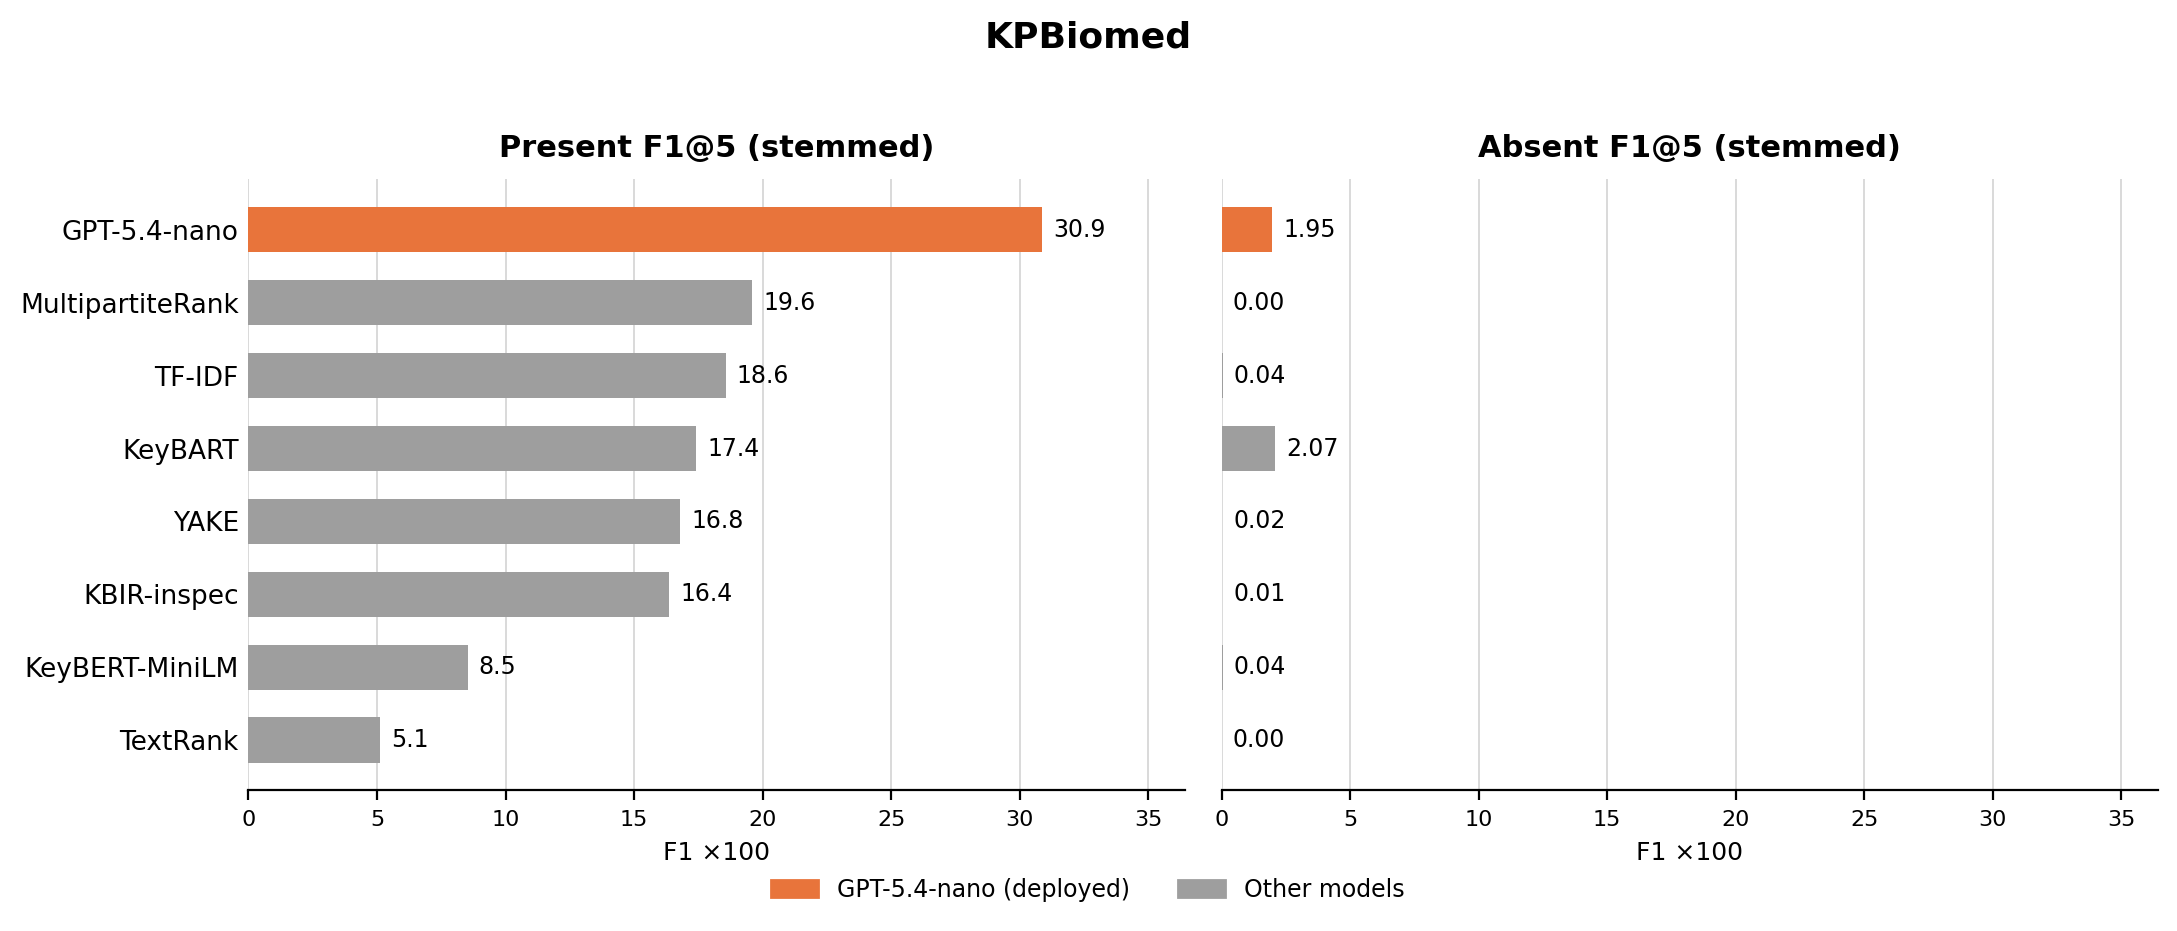
\includegraphics[width=\textwidth]{images/data_and_results/keyword_kpbiomed.png}
\caption{KPBiomed keyword extraction, present and absent F1@5 by model with stemming. The deployed model GPT-5.4-nano is shown in orange and the remaining baselines in grey.}
\label{fig:kw-kpbiomed}
\end{figure*}

\begin{table}[t]
\caption{OAGKX keyword extraction, present and absent F1@5 with stemming. Models are ordered by present F1, and GPT-5.4-nano is the deployed model.}
\label{tab:kw-oagkx}
\centering
\footnotesize
\begin{tabular}{@{}lrr@{}}
\toprule
Model & Present F1@5 & Absent F1@5 \\
\midrule
KeyBART & \textbf{28.42} & \textbf{5.09} \\
\textbf{GPT-5.4-nano} & 26.49 & 1.77 \\
KBIR-inspec & 20.16 & 0.05 \\
MultipartiteRank & 18.83 & 0.00 \\
TF-IDF & 15.55 & 0.03 \\
KeyBERT-MiniLM & 12.04 & 0.04 \\
TextRank & 11.15 & 0.02 \\
YAKE & 8.85 & 0.00 \\
\bottomrule
\end{tabular}
\end{table}

\begin{figure*}[t]
\centering
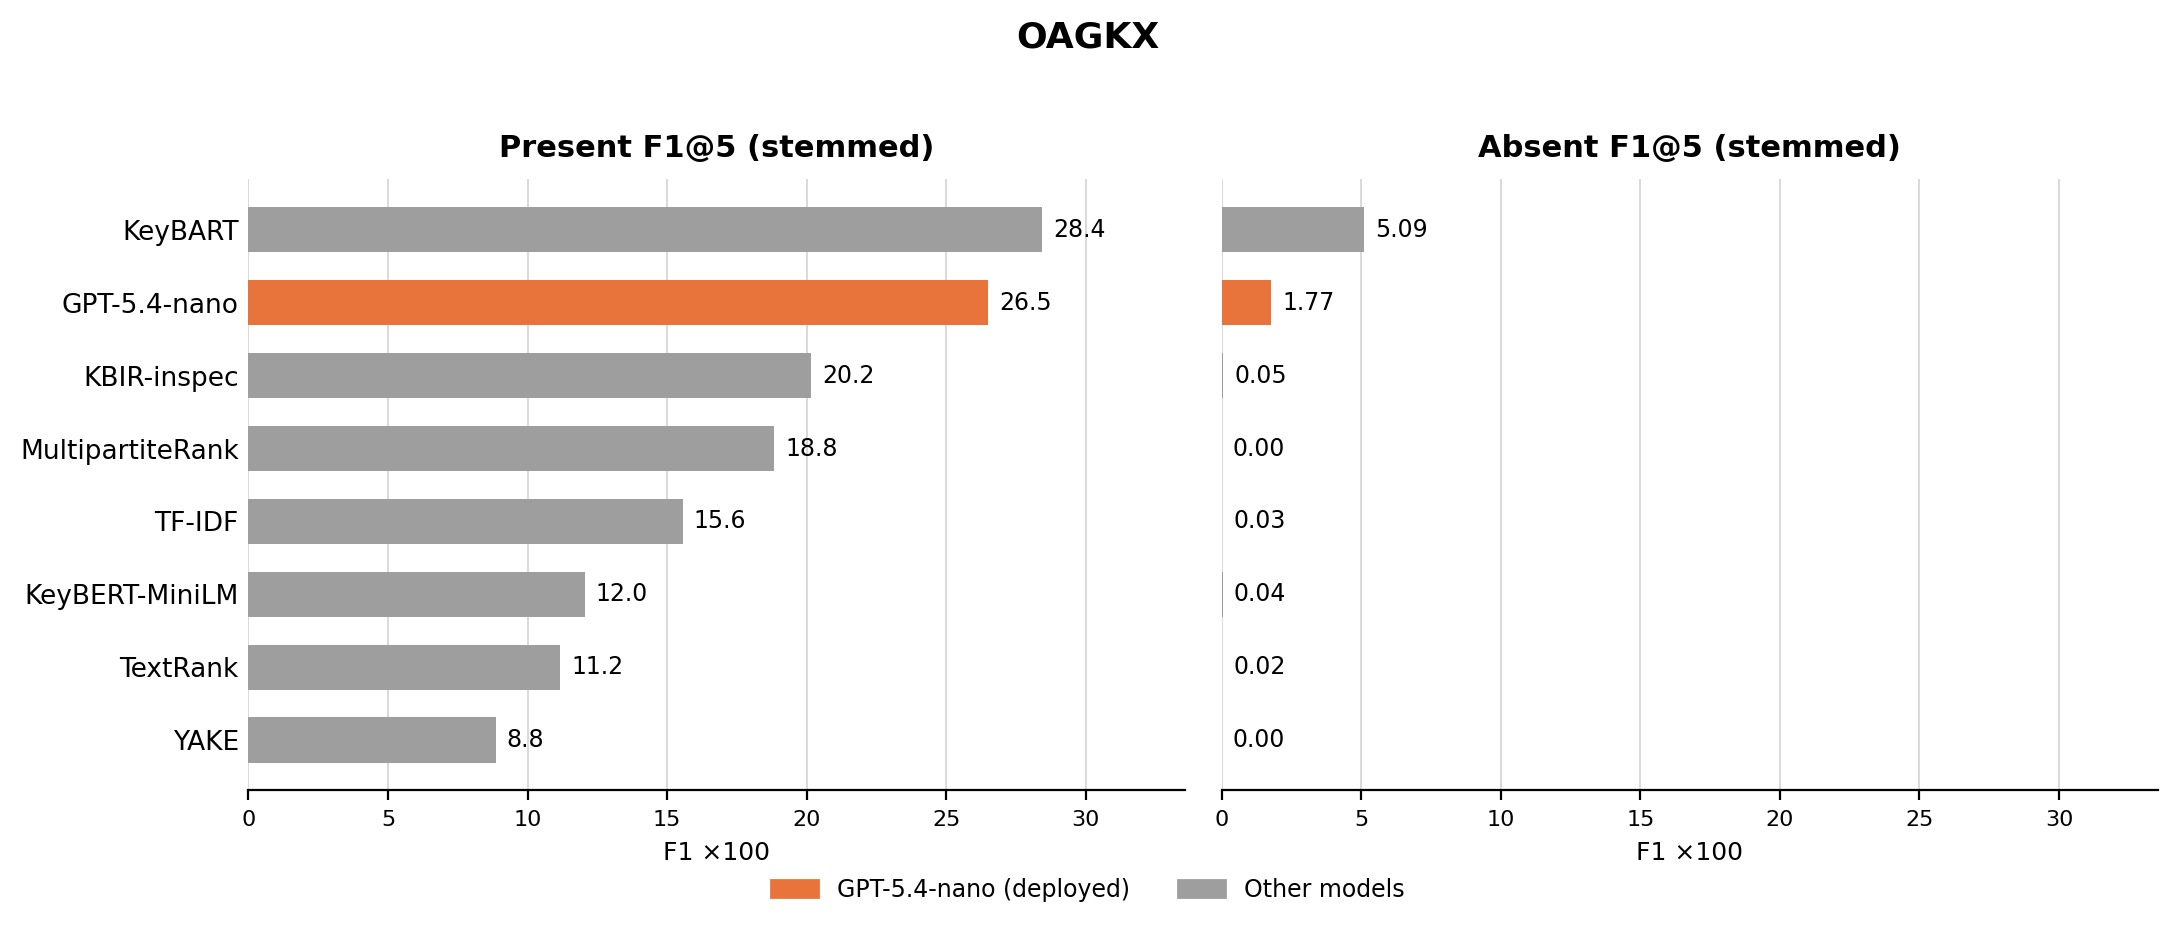
\includegraphics[width=\textwidth]{images/data_and_results/keyword_oagkx.png}
\caption{OAGKX keyword extraction, present and absent F1@5 by model with stemming. The deployed model GPT-5.4-nano is shown in orange and the remaining baselines in grey.}
\label{fig:kw-oagkx}
\end{figure*}

\begin{table}[t]
\caption{PubMedAKE keyword extraction, present and absent F1@5 with stemming. Models are ordered by present F1, and GPT-5.4-nano is the deployed model.}
\label{tab:kw-pubmedake}
\centering
\footnotesize
\begin{tabular}{@{}lrr@{}}
\toprule
Model & Present F1@5 & Absent F1@5 \\
\midrule
\textbf{GPT-5.4-nano} & \textbf{36.44} & \textbf{1.30} \\
TF-IDF & 24.06 & 0.03 \\
MultipartiteRank & 23.06 & 0.00 \\
KBIR-inspec & 19.36 & 0.01 \\
KeyBART & 18.41 & 1.29 \\
YAKE & 12.92 & 0.01 \\
KeyBERT-MiniLM & 6.78 & 0.01 \\
TextRank & 4.68 & 0.00 \\
\bottomrule
\end{tabular}
\end{table}

\begin{figure*}[t]
\centering
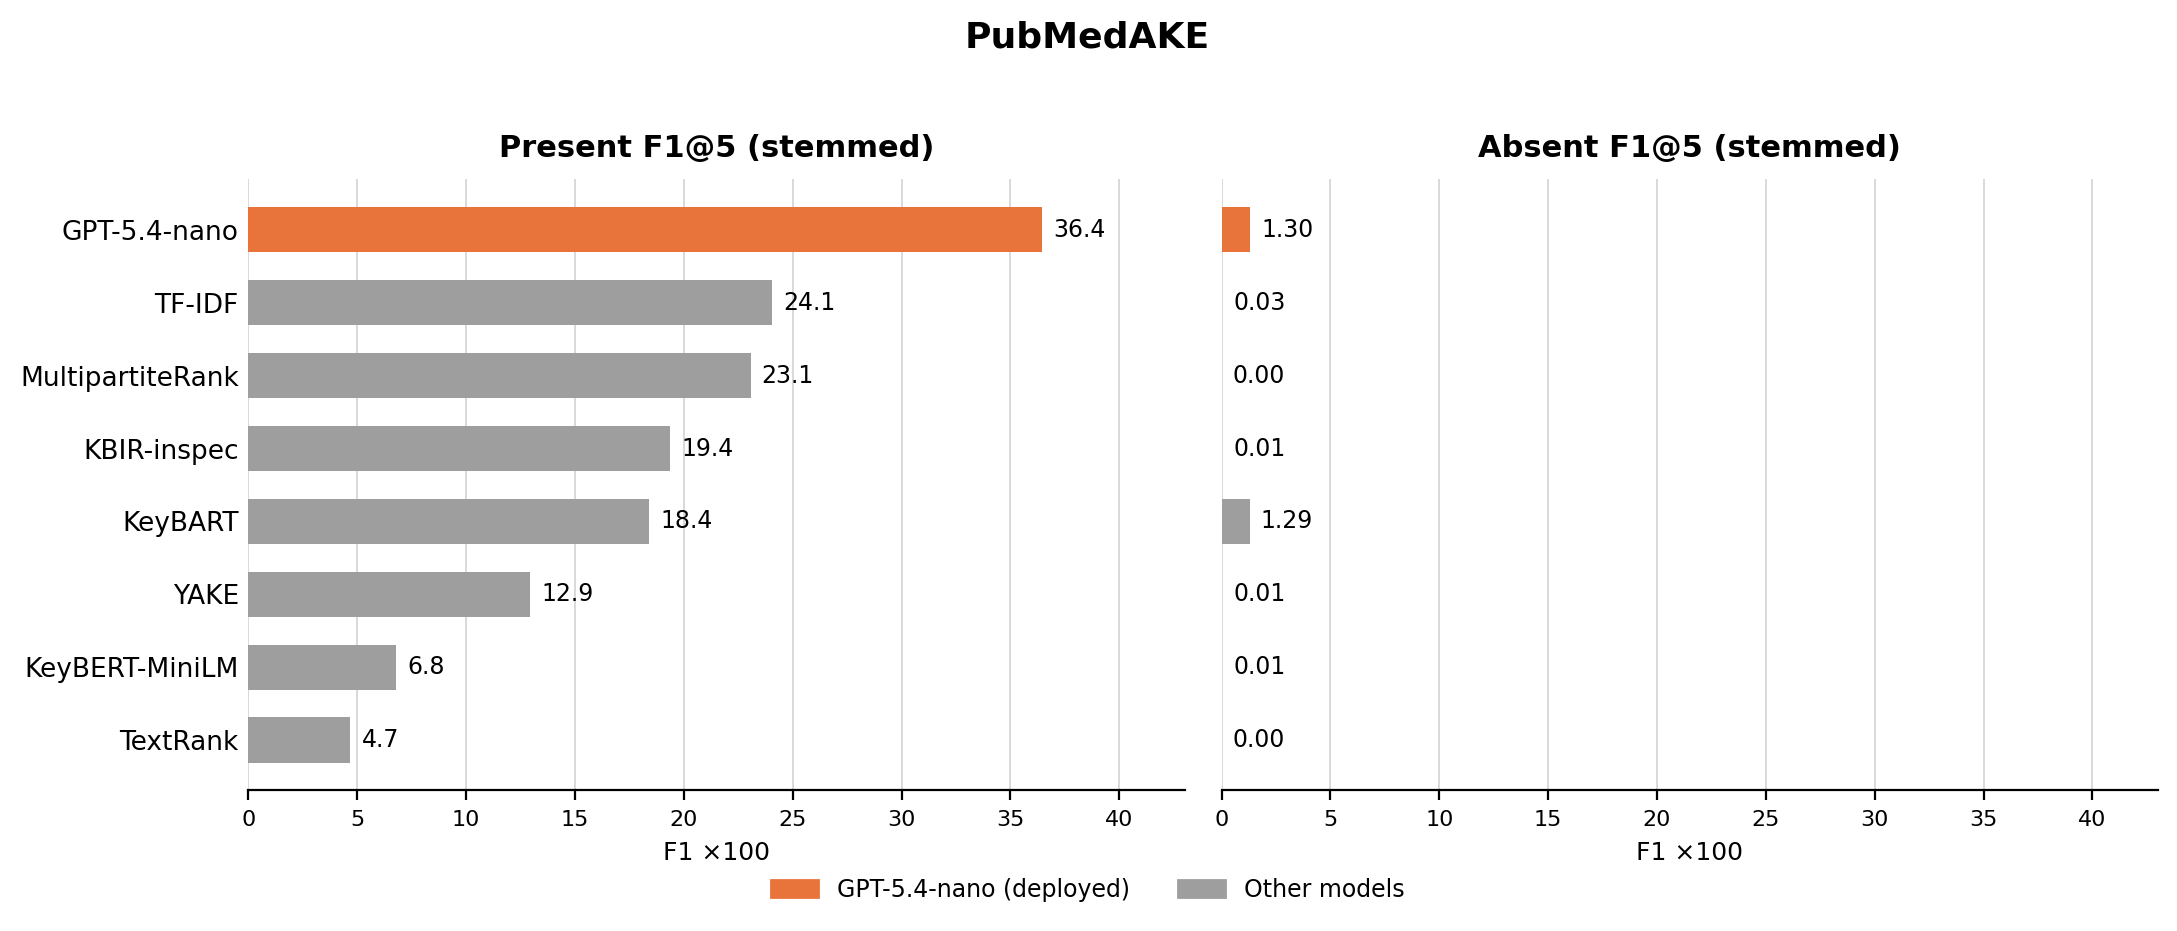
\includegraphics[width=\textwidth]{images/data_and_results/keyword_pubmedake.png}
\caption{PubMedAKE keyword extraction, present and absent F1@5 by model with stemming. The deployed model GPT-5.4-nano is shown in orange and the remaining baselines in grey.}
\label{fig:kw-pubmedake}
\end{figure*}

GPT-5.4-nano was benchmarked for keyword generation against a set of statistical and neural baselines on KPBiomed, OAGKX, and PubMedAKE. Tables~\ref{tab:kw-kpbiomed} to~\ref{tab:kw-pubmedake} report the results for each dataset in turn. Throughout, present (extractive) keyphrases, which occur verbatim in the source text, are distinguished from absent (abstractive) keyphrases, which do not and so must be generated. Matches are scored by F1 at five with light stemming, so that a keyphrase and its stem count as a match while a different word of the same meaning does not.

On the present keyphrase tasks, GPT-5.4-nano records the highest score on KPBiomed and PubMedAKE and the second highest on OAGKX, where KeyBART leads. Its margin is widest on PubMedAKE, at 36.44 against a next-best of 24.06.

On the absent keyphrase tasks, which a model can only score on by producing keyphrases that do not occur in the source text, GPT-5.4-nano scores in the low single digits, from 1.30 on PubMedAKE to 1.95 on KPBiomed. These non-zero scores indicate that the model generates a small portion of its keyphrases rather than extracting all of them. The other generative baseline, KeyBART, behaves similarly and records the highest absent score on KPBiomed and OAGKX. The statistical extractors such as TF-IDF, YAKE, TextRank, and MultipartiteRank remain near zero here, since they return only spans found in the source text and so do not generate at all.

\begin{table}[t]
\caption{Keyword extraction stability for GPT-5.4-nano over three runs on a 2000-document sample.}
\label{tab:kw-stability}
\centering
\footnotesize
\begin{tabular}{@{}p{0.66\columnwidth}r@{}}
\toprule
Quantity & Value \\
\midrule
Set-level Jaccard across runs & 0.73 \\
Present-F1 run-to-run std & $\pm$0.07 \\
Deterministic baselines (TF-IDF, YAKE, TextRank, MultipartiteRank, KeyBERT, KBIR) & 1.00 \\
\bottomrule
\end{tabular}
\end{table}

Table~\ref{tab:kw-stability} reports a reproducibility check for GPT-5.4-nano over three runs on a 2000-document sample. The set-level Jaccard similarity across runs is 0.73, meaning that for a given document around 73 percent of the combined set of keyphrases from any two runs is shared by both, equivalent to roughly one in six keyphrases changing between runs. The model is therefore largely repeatable but not deterministic, unlike the baselines, which are reproducible by construction. The effect on measured performance is negligible, with a run-to-run present-F1 standard deviation of 0.07. The same sample also reproduces the full-split figures to within roughly a tenth of a point, confirming that the smaller stability sample does not shift the headline results.

% ----------------------------------------------------------------------------
\subsection{IR Extraction}

\begin{table*}[t]
\caption{Natural-language-to-IR accuracy by model. Joint IR accuracy counts a query as correct when both its entities and its boolean expression are correct under exact matching, reported in the as-deployed or best configuration for each model.}
\label{tab:ir-accuracy}
\centering
\footnotesize
\begin{tabular}{@{}lllcc@{}}
\toprule
Model & Host & Configuration & IR accuracy & 95\% CI \\
\midrule
\textbf{gpt-5.4-nano} & Azure & default, 0 reasoning tok & \textbf{0.937}$^{\dagger}$ & [0.897, 0.983] \\
gpt-5-mini & Azure & default, 384 reasoning tok & 0.931 & [0.879, 0.974] \\
qwen3:8b & Local (Q4) & single-shot & 0.802 & [0.733, 0.871] \\
qwen3:4b & Local (Q4) & thinking$^{\ddagger}$ & 0.784 & [0.707, 0.862] \\
qwen2.5:3b & Local (Q4) & non-reasoning & 0.207 & [0.138, 0.284] \\
phi4-mini & Local (Q4) & non-reasoning & 0.052 & [0.017, 0.095] \\
llama3.2:3b & Local (Q4) & non-reasoning & 0.026 & [0.000, 0.060] \\
\bottomrule
\end{tabular}

\vspace{3pt}
\begin{minipage}{\linewidth}
\footnotesize\itshape
Confidence intervals are 95 percent bootstrap over 1000 iterations. Cross-model gaps that fall within these intervals are treated as ties, and bold marks the deployed model. The dagger denotes a three-run mean, whose single-run range is 0.914 to 0.940, with temperature zero returning a byte-identical output on 96.6 percent of queries (Table~\ref{tab:ir-stability}). The double dagger denotes qwen3:4b, whose single-shot configuration produced degenerate empty output, so its thinking configuration is its only usable score.
\end{minipage}
\end{table*}

\begin{figure}[t]
\centering
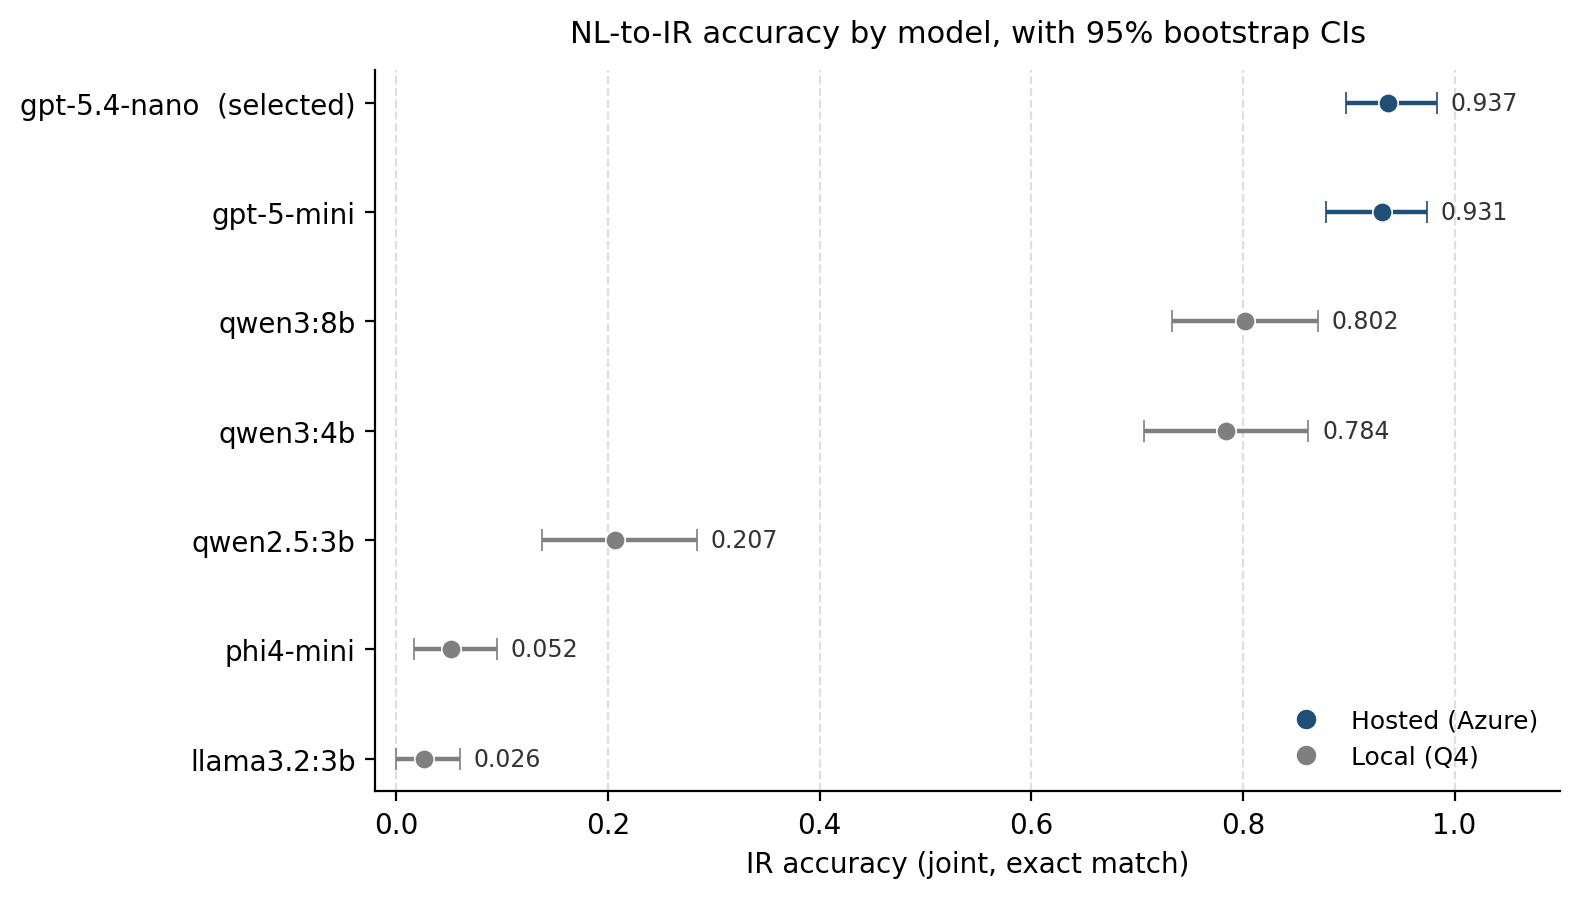
\includegraphics[width=\columnwidth]{images/data_and_results/ir_accuracy_ci.png}
\caption{Natural-language-to-IR joint accuracy by model on the hand-built gold set, with 95 percent bootstrap confidence intervals from 1000 resamples.}
\label{fig:ir-accuracy}
\end{figure}

GPT-5.4-nano was benchmarked for natural-language-to-IR extraction against a set of hosted and local models on a hand-built gold set of queries paired with their correct intermediate representations. The set was constructed to exercise every entity type the system supports across a range of boolean structures, from single topics through to bracketed combinations of AND, OR, and NOT, so that performance on it reflects the input and output behaviour the system actually requires. The headline measure, IR accuracy, is the joint figure reported in Table~\ref{tab:ir-accuracy}, counting a query as correct only when both its extracted entities and its boolean expression are correct under exact matching.

Figure~\ref{fig:ir-accuracy} plots each model's accuracy with its 95 percent bootstrap interval. The two hosted models lead the benchmark by a clear margin, with GPT-5.4-nano highest at an IR accuracy of 0.937 and GPT-5-mini close behind at 0.931. Both hosted intervals clear those of every local model without overlap, placing the hosted advantage beyond sampling noise, while the two overlap each other and are statistically indistinguishable. Among the local models, the two strongest (qwen3:8b and qwen3:4b) reach around 0.80, and the three smaller models fall away sharply to 0.207, 0.052, and 0.026, near the floor of the task.

\begin{table}[t]
\caption{Effect of reasoning on IR accuracy.}
\label{tab:ir-reasoning}
\centering
\footnotesize
\begin{tabular}{@{}lccc@{}}
\toprule
Model & Reasoning off & Reasoning on & $\Delta$ \\
\midrule
gpt-5.4-nano & 0.914 & 0.922 & +0.008 \\
gpt-5-mini & \textbf{0.750} & \textbf{0.940} & \textbf{+0.190} \\
\bottomrule
\end{tabular}

\vspace{3pt}
\begin{minipage}{\linewidth}
\footnotesize\itshape
Reasoning is controlled through the Azure \texttt{reasoning\_effort} setting with tokens accounted. Reasoning on used approximately 246 tokens per query for gpt-5.4-nano and 896 for gpt-5-mini, while reasoning off used none. Reasoning lifts the weaker model in each tier, while the stronger one is already at its ceiling.
\end{minipage}
\end{table}

Table~\ref{tab:ir-reasoning} isolates the effect of reasoning on the two GPT models. GPT-5.4-nano gains almost nothing from it, moving from 0.914 without reasoning to 0.922 with around 246 reasoning tokens, a difference of 0.008, and so reaches its accuracy in a single pass with no reasoning budget. GPT-5-mini behaves differently, scoring only 0.750 without reasoning and rising to 0.940 once reasoning is enabled, at a cost of around 896 reasoning tokens per query. The stronger model is already at its ceiling unaided, whereas the weaker one becomes competitive only by spending a substantial token budget.

\begin{table}[t]
\caption{Deployed model, metric decomposition in the default-effort configuration.}
\label{tab:ir-decomp}
\centering
\footnotesize
\begin{tabular}{@{}lcc@{}}
\toprule
Metric & Value & 95\% CI \\
\midrule
IR accuracy (joint) & 0.937 & [0.897, 0.983] \\
Entity F1 (micro) & 0.984 & [0.969, 0.995] \\
Entity F1 (macro) & 0.982 & [0.967, 0.994] \\
Expression equivalence & 0.931 & [0.888, 0.974] \\
Expression graded & 0.985 & [0.974, 0.995] \\
\bottomrule
\end{tabular}

\vspace{3pt}
\begin{minipage}{\linewidth}
\footnotesize\itshape
Joint accuracy is bounded by expression equivalence, since entity extraction almost never fails on its own.
\end{minipage}
\end{table}

\begin{table}[t]
\caption{Deployed model, accuracy by stratum, ordered hardest first.}
\label{tab:ir-stratum}
\centering
\footnotesize
\begin{tabular}{@{}lrrr@{}}
\toprule
Stratum & $n$ & IR accuracy & failures \\
\midrule
\texttt{filter\_distractor} & 10 & 0.700 & 3 \\
\texttt{multi\_negation} & 10 & 0.800 & 2 \\
\texttt{deep\_nested} & 12 & 0.833 & 2 \\
\texttt{hard\_typing} & 12 & 0.917 & 1 \\
\texttt{single\_concept} & 6 & 1.000 & 0 \\
\texttt{multi\_concept} & 12 & 1.000 & 0 \\
\texttt{exclusion} & 12 & 1.000 & 0 \\
\texttt{nested} & 12 & 1.000 & 0 \\
\texttt{mixed\_entity} & 16 & 1.000 & 0 \\
\texttt{review\_style} & 14 & 1.000 & 0 \\
\bottomrule
\end{tabular}

\vspace{3pt}
\begin{minipage}{\linewidth}
\footnotesize\itshape
The count $n$ is small per stratum, at sixteen or fewer, so the failure counts are a more reliable read than the rate, and the per-stratum 95 percent intervals are wide, for example \texttt{filter\_distractor} at 0.700 is seven of ten.
\end{minipage}
\end{table}

Tables~\ref{tab:ir-decomp} and~\ref{tab:ir-stratum} decompose the chosen model's performance, which is strong across both components and most query types. By component, entity extraction is near-perfect, with a micro F1 of 0.984 and a macro F1 of 0.982, while expression equivalence is lower at 0.931 (a graded variant that credits partially correct expressions reaches 0.985). The joint IR accuracy of 0.937 is therefore bounded by the expression score, since entity extraction almost never fails on its own. By query type, the model is perfect on six of the ten strata, covering single and multiple concepts, exclusions, nesting, mixed entities, and review-style queries. Its errors concentrate in the remaining four. The largest source is \texttt{filter\_distractor}, where three of ten queries fail because the model miscategorises a filter term such as a year or citation bound as a searchable entity. The rest fall on the structurally hardest queries, with two of ten failing on multiple negations, two of twelve on deep nesting, and one of twelve on hard typing. Per-stratum counts are small, at sixteen queries or fewer, so the failure counts are a more reliable read than the rates.

\begin{table}[t]
\caption{Stability of the deployed model over three runs.}
\label{tab:ir-stability}
\centering
\footnotesize
\begin{tabular}{@{}p{0.46\columnwidth}cc@{}}
\toprule
Metric & temp 0 & temp 0.7 \\
\midrule
IR identical across all 3 runs & 0.966 & 0.957 \\
Run-to-run IR-accuracy std & 0.004 & 0.004 \\
Majority-vote@3 vs single run & 0.931 vs 0.940 & 0.940 vs 0.940 \\
\bottomrule
\end{tabular}

\vspace{3pt}
\begin{minipage}{\linewidth}
\footnotesize\itshape
Temperature zero is highly but not perfectly deterministic, and majority voting adds nothing.
\end{minipage}
\end{table}

Table~\ref{tab:ir-stability} reports a stability check over three runs. Although GPT-5.4-nano is not deterministic, at temperature zero it returns an identical IR on 96.6 percent of queries, with a run-to-run accuracy standard deviation of 0.004. Aggregating three runs by majority vote changes nothing, at 0.931 against 0.940 for a single run, so the three-run mean of 0.937 reported in Table~\ref{tab:ir-accuracy} is used throughout.

% ----------------------------------------------------------------------------
\subsection{Dense Bi-encoder Retrieval}

\begin{table*}[t]
\caption{Dense bi-encoder retrieval on SciRepEval ad-hoc search, nDCG $\times$100 with 95 percent bootstrap confidence intervals.}
\label{tab:bienc-results}
\centering
\scriptsize
\setlength{\tabcolsep}{4pt}
\begin{tabular}{@{}p{3.0cm}llll@{}}
\toprule
Model & NFCorpus & TREC-CoVID & Search & Average \\
\midrule
Qwen3-Embedding-4B (int8) & \textbf{80.02 [77.75, 82.17]} & \textbf{94.28 [92.96, 95.43]} & 75.54 [74.93, 76.17] & \textbf{83.28 [82.35, 84.19]} \\
EmbeddingGemma-300M & 79.13 [76.84, 81.29] & 92.45 [90.68, 94.03] & 75.32 [74.66, 75.93] & 82.30 [81.32, 83.31] \\
Qwen3-Embedding-0.6B & 77.94 [75.75, 80.22] & 93.90 [92.52, 95.10] & 75.03 [74.41, 75.65] & 82.29 [81.32, 83.25] \\
text-embedding-3-small (existing) & 78.78 [76.61, 81.05] & 92.38 [90.58, 93.96] & 75.14 [74.52, 75.74] & 82.10 [81.08, 83.05] \\
mxbai-embed-large-v1 & 79.37 [77.19, 81.72] & 91.77 [90.02, 93.25] & 74.92 [74.29, 75.56] & 82.02 [81.06, 82.96] \\
SPECTER2-adhoc-query & 70.46 [68.01, 72.97] & 90.08 [87.84, 92.13] & \textbf{78.22 [77.60, 78.86]} & 79.59 [78.46, 80.71] \\
BGE-M3 & 74.05 [71.72, 76.35] & 89.21 [87.08, 91.16] & 74.82 [74.20, 75.46] & 79.36 [78.29, 80.42] \\
SPECTER2-base (existing) & 72.03 [69.60, 74.54] & 89.46 [86.99, 91.58] & 73.76 [73.12, 74.41] & 78.42 [77.27, 79.58] \\
\bottomrule
\end{tabular}

\vspace{3pt}
\begin{minipage}{\linewidth}
\footnotesize\itshape
The metric is SciRepEval ad-hoc-search full-ranking nDCG over a per-query candidate pool, not BEIR full-corpus nDCG@10. Confidence intervals are 95 percent bootstrap [lo, hi] over 1000 iterations with seed 42, and bold marks the best point estimate per column. On Average the top five models' intervals overlap, a statistical tie, and SPECTER2-adhoc-query's Search lead is the one between-model gap whose interval clears the general models.
\end{minipage}
\end{table*}

\begin{figure}[t]
\centering
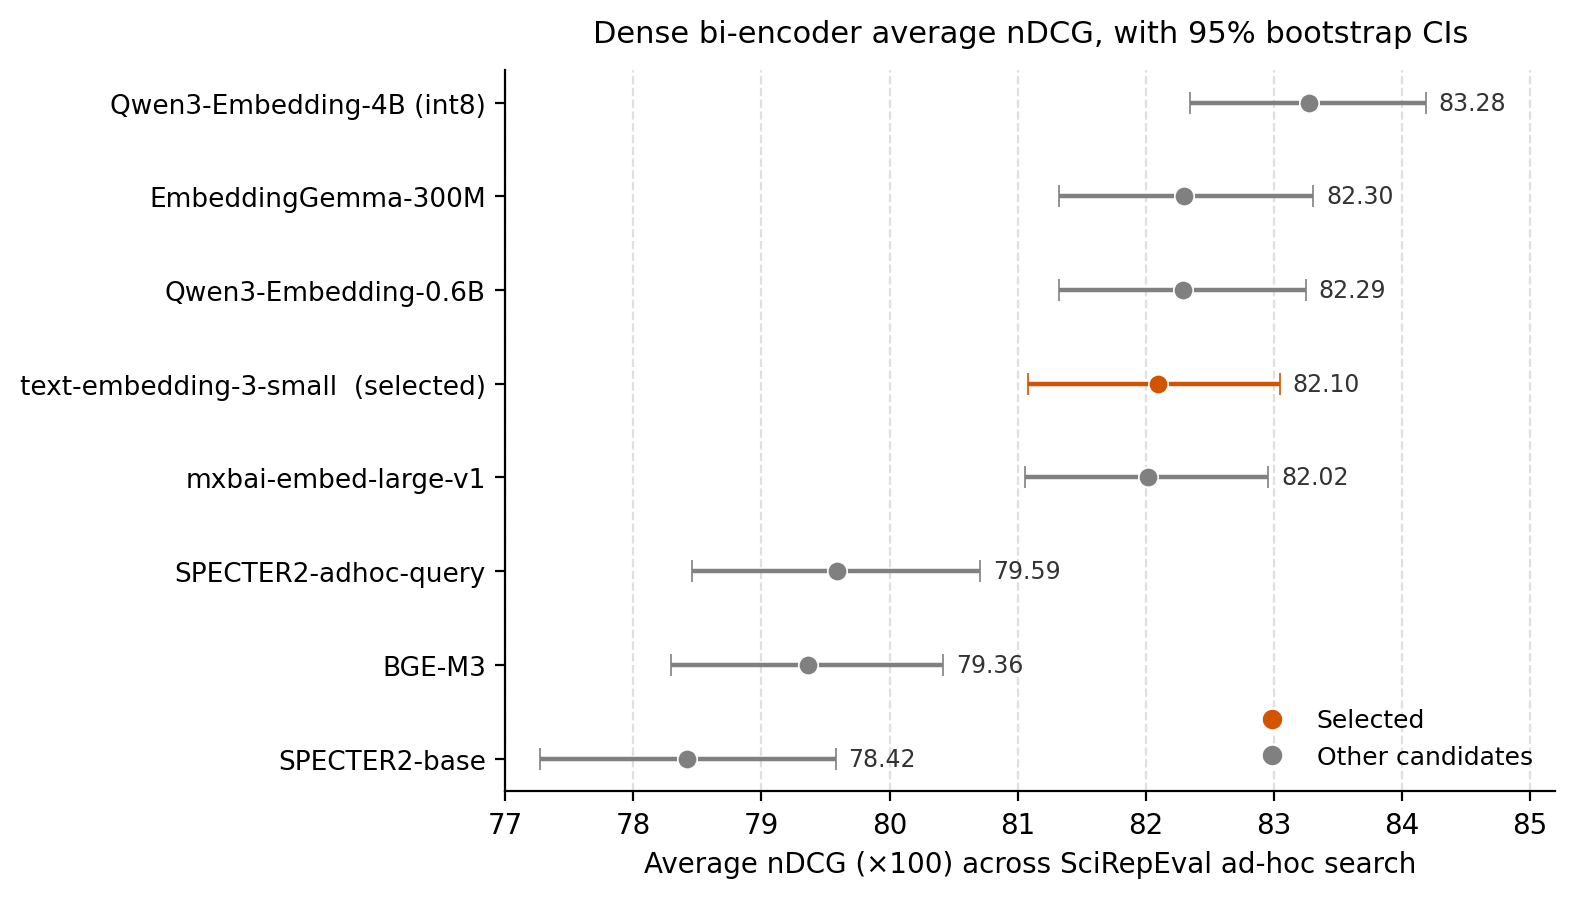
\includegraphics[width=\columnwidth]{images/data_and_results/biencoder_average.png}
\caption{Dense bi-encoder average nDCG across the three SciRepEval ad-hoc search tasks, with 95 percent bootstrap confidence intervals from 1000 resamples. The selected model is shown in orange.}
\label{fig:bienc-avg}
\end{figure}

\begin{figure}[t]
\centering
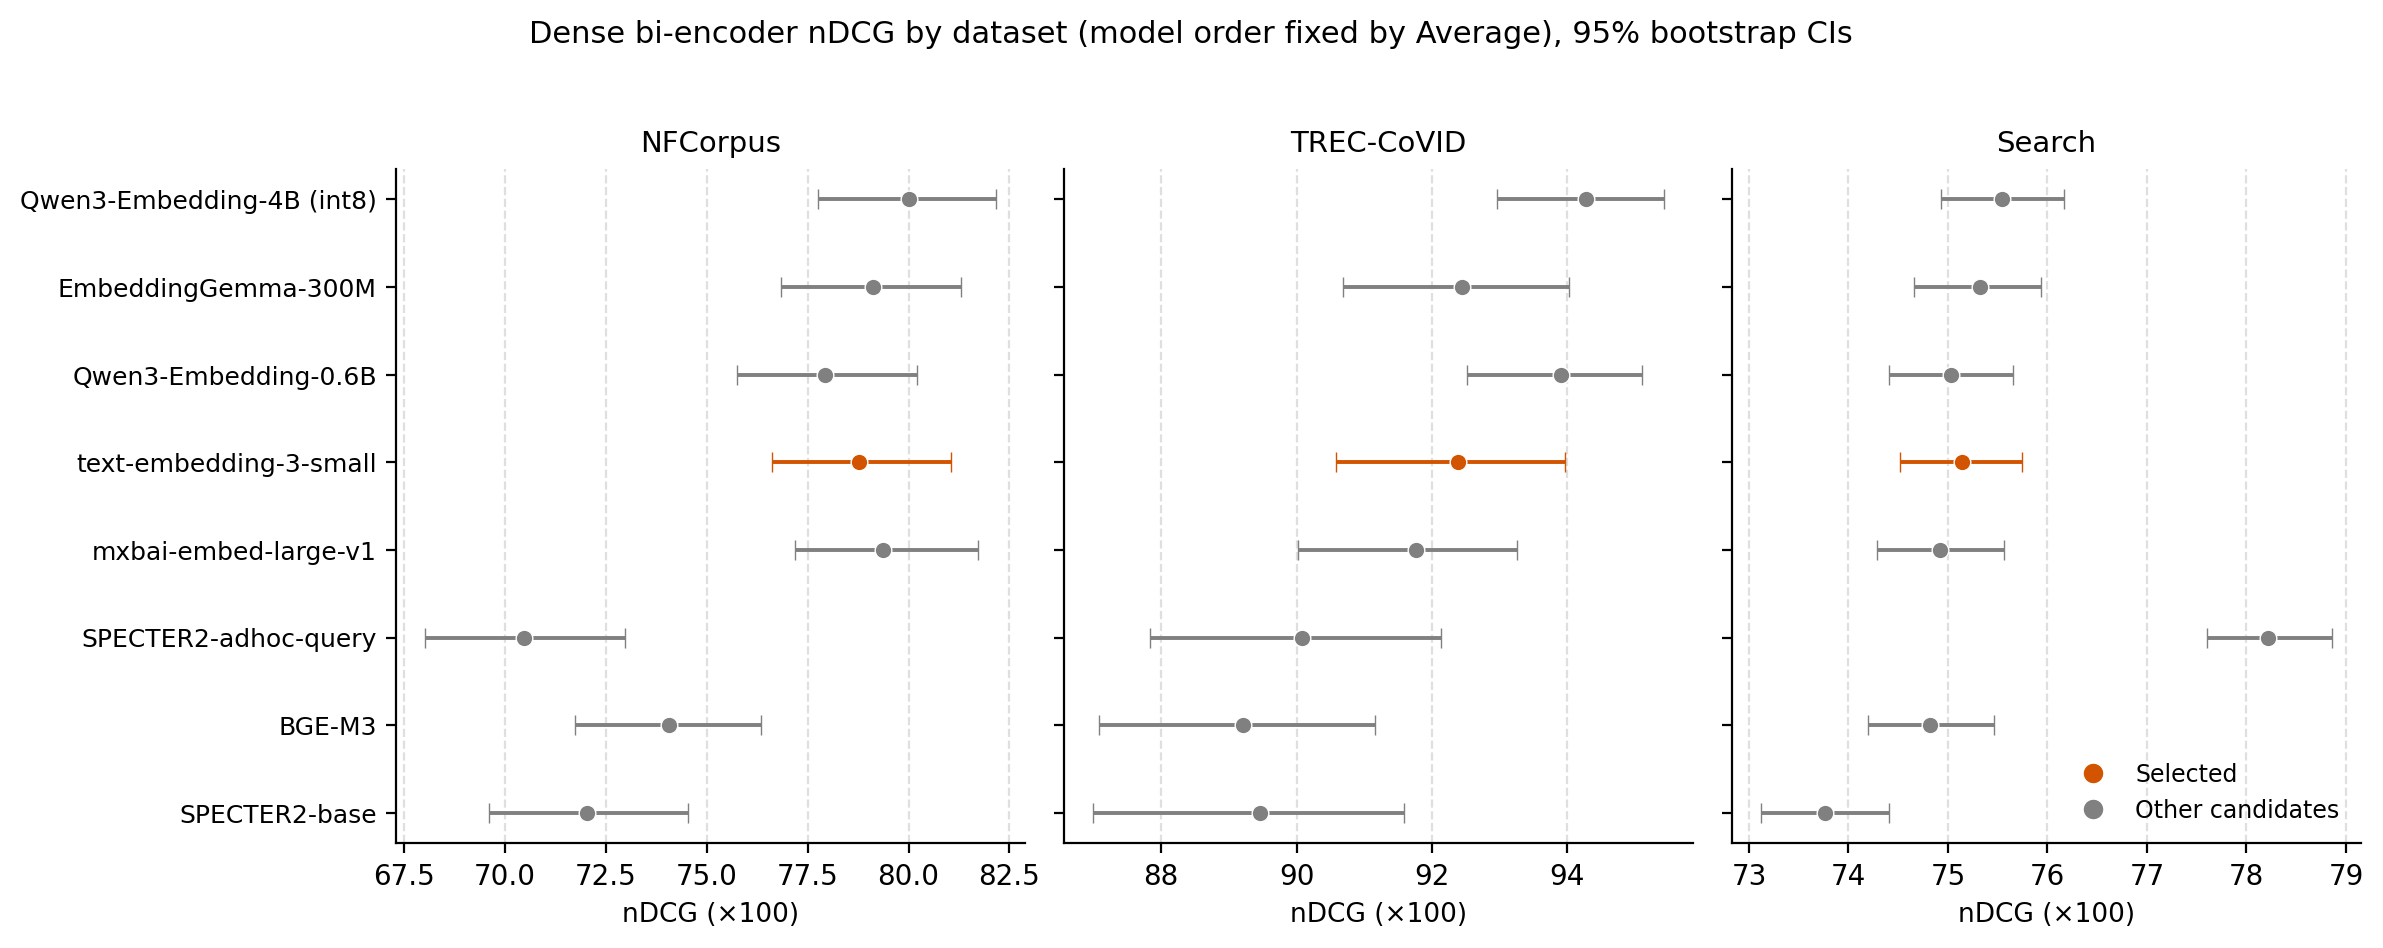
\includegraphics[width=\columnwidth]{images/data_and_results/biencoder_by_dataset.png}
\caption{Dense bi-encoder nDCG on each SciRepEval ad-hoc search task, with models held in their Average order for comparison and 95 percent bootstrap confidence intervals. The selected model is shown in orange.}
\label{fig:bienc-pertask}
\end{figure}

text-embedding-3-small was selected as the dense bi-encoder. The candidate models were evaluated on the three ad-hoc search tasks of SciRepEval, namely NFCorpus, TREC-CoVID, and Search, scored by nDCG. The figure reported is SciRepEval full-ranking nDCG over a per-query candidate pool rather than BEIR full-corpus nDCG@10, which keeps the stage comparable to the scientific retrieval benchmark established in Section~II-D. All scores are nDCG $\times$100 with 95 percent bootstrap intervals from 1000 resamples.

Table~\ref{tab:bienc-results} reports the per-task and average scores in full, and Figure~\ref{fig:bienc-avg} plots each model's average nDCG with its interval. The selected model records an average of 82.10. Qwen3-Embedding-4B holds the highest point estimate at 83.28, but the intervals of the top five models all overlap, forming a statistical tie that contains text-embedding-3-small along with EmbeddingGemma-300M, Qwen3-Embedding-0.6B, and mxbai-embed-large-v1. A clear margin separates this group from the lower three, SPECTER2-adhoc-query at 79.59, BGE-M3 at 79.36, and SPECTER2-base at 78.42, whose intervals fall below the leading cluster.

The average conceals a difference in where each model does its work, shown per task in Figure~\ref{fig:bienc-pertask}. On NFCorpus and TREC-CoVID the general-purpose embedders lead, with Qwen3-Embedding-4B highest on both. On Search the order changes. SPECTER2-adhoc-query scores 78.22 against a field clustered near 75, and this is the single between-model gap on any one task whose interval clears the general models. The same model is weakest on NFCorpus at 70.46, so its Search lead does not survive into the average. The selected model sits within the leading group on each of the three tasks.

\begin{table*}[t]
\caption{Deployment characteristics of the candidate bi-encoders.}
\label{tab:bienc-deploy}
\centering
\footnotesize
\begin{tabular}{@{}lllll@{}}
\toprule
Model & Params (approx.) & Embedding dim & Precision & Self-hostable \\
\midrule
Qwen3-Embedding-4B & $\sim$4 B & 2560 & int8 & yes \\
EmbeddingGemma-300M & $\sim$300 M & 768 & fp16 & yes \\
Qwen3-Embedding-0.6B & $\sim$0.6 B & 1024 & fp16 & yes \\
text-embedding-3-small & undisclosed & 1536 & n/a & no (paid API) \\
mxbai-embed-large-v1 & $\sim$335 M & 1024 & fp16 & yes \\
SPECTER2-adhoc-query & $\sim$110 M & 768 & fp16 & yes \\
BGE-M3 & $\sim$568 M & 1024 & fp16 & yes \\
SPECTER2-base & $\sim$110 M & 768 & fp16 & yes \\
\bottomrule
\end{tabular}

\vspace{3pt}
\begin{minipage}{\linewidth}
\footnotesize\itshape
In-memory footprint per stored vector scales with embedding dimension at int8, at roughly one byte per dimension, giving around 65 GB at 768 dimensions, 87 GB at 1024, 131 GB at 1536, and 218 GB at 2560 over the 85 million works. Encoding cost scales with parameter count.
\end{minipage}
\end{table*}

Table~\ref{tab:bienc-deploy} records the deployment characteristics that the nDCG scores do not, namely approximate parameter count, embedding dimension, precision, and whether the model is self-hostable. In-memory footprint per stored vector scales with embedding dimension at int8, from around 65 GB at 768 dimensions to around 218 GB at 2560 dimensions over the 85 million works, while encoding cost scales with parameter count. The selected model has an embedding dimension of 1536, placing its footprint at around 131 GB, and is served through a paid API rather than self-hosted.

% ----------------------------------------------------------------------------
\subsection{Cross-encoder Re-ranking}

\begin{table*}[t]
\caption{Cross-encoder re-ranking on SciRepEval ad-hoc search, nDCG $\times$100 with 95 percent bootstrap confidence intervals, sorted by Average.}
\label{tab:xenc-results}
\centering
\scriptsize
\setlength{\tabcolsep}{4pt}
\begin{tabular}{@{}p{3.2cm}llll@{}}
\toprule
Model (scorer) & NFCorpus & TREC-CoVID & Search & Average \\
\midrule
Cohere Rerank 4.0 Pro (API) & \textbf{80.42 [78.17, 82.60]} & \textbf{94.60 [93.30, 95.71]} & 75.39 [74.76, 76.00] & \textbf{83.47 [82.54, 84.33]} \\
Qwen3-Reranker-4B (int8) & 80.10 [77.94, 82.14] & 94.37 [92.90, 95.60] & 74.93 [74.32, 75.56] & 83.13 [82.18, 83.99] \\
Cohere Rerank 4.0 Fast (API) & 78.77 [76.55, 80.98] & 94.15 [92.83, 95.31] & \textbf{75.42 [74.75, 76.04]} & 82.78 [81.83, 83.68] \\
Qwen3-Reranker-0.6B (fp16) & 78.06 [75.65, 80.24] & 93.98 [92.59, 95.20] & 75.25 [74.59, 75.85] & 82.43 [81.50, 83.34] \\
mxbai-rerank-large-v1 (435M) & 78.32 [76.08, 80.76] & 91.50 [89.43, 93.33] & 74.78 [74.15, 75.46] & 81.53 [80.48, 82.59] \\
jina-reranker-v2-base (278M) & 76.73 [74.49, 79.01] & 91.84 [90.05, 93.52] & 75.37 [74.73, 75.99] & 81.31 [80.28, 82.30] \\
MedCPT-Cross-Encoder (109M, biomed) & 75.70 [73.21, 78.03] & 88.91 [86.61, 90.97] & 73.97 [73.34, 74.63] & 79.53 [78.40, 80.66] \\
ms-marco-MiniLM-L-6-v2 (22M) & 73.10 [70.78, 75.48] & 88.78 [86.41, 90.90] & 75.21 [74.58, 75.84] & 79.03 [77.90, 80.13] \\
bge-reranker-v2-m3 (568M) & 70.71 [68.31, 73.07] & 90.30 [88.29, 92.18] & 74.40 [73.78, 75.05] & 78.47 [77.37, 79.53] \\
ms-marco-MiniLM-L-12-v2 (33M) & 69.88 [67.41, 72.38] & 87.17 [84.73, 89.52] & 75.09 [74.44, 75.71] & 77.38 [76.17, 78.54] \\
bge-reranker-large (560M) & 66.49 [64.11, 68.85] & 87.27 [84.61, 89.62] & 74.22 [73.59, 74.85] & 76.00 [74.80, 77.16] \\
bge-reranker-base (278M) & 58.75 [56.38, 60.94] & 84.98 [82.12, 87.60] & 72.60 [71.97, 73.24] & 72.11 [70.84, 73.35] \\
gte-reranker-modernbert-base (150M) & 48.88 [46.82, 50.93] & 79.03 [76.40, 81.60] & 69.94 [69.26, 70.60] & 65.95 [64.91, 67.07] \\
\bottomrule
\end{tabular}

\vspace{3pt}
\begin{minipage}{\linewidth}
\footnotesize\itshape
The metric is SciRepEval ad-hoc-search full-ranking nDCG over a reranking pool, not BEIR full-corpus nDCG@10. Confidence intervals are 95 percent bootstrap [2.5 percent, 97.5 percent] over 1000 iterations with seed 42, with the Average resampled independently within each dataset. The intervals are tight on Search, which has 2585 queries, and wide on TREC-CoVID, which has 50, and bold marks the best point estimate per column. The top four models, namely Cohere Pro, Qwen3-Reranker-4B, Cohere Fast, and Qwen3-Reranker-0.6B, have heavily overlapping Average intervals and form a statistical tie, within which the best self-hostable model, Qwen3-Reranker-4B at int8, is tied with Cohere Pro. On Search the small candidate pool saturates every reranker at around 75. For reference, the bi-encoder embeddings without intervals give the best embedder Qwen3-Embedding-4B at 83.28 Average, SPECTER2-adhoc-query at 78.22 on Search, which is above every reranker here, and text-embedding-3-small at 82.10 Average.
\end{minipage}
\end{table*}

\begin{figure}[t]
\centering
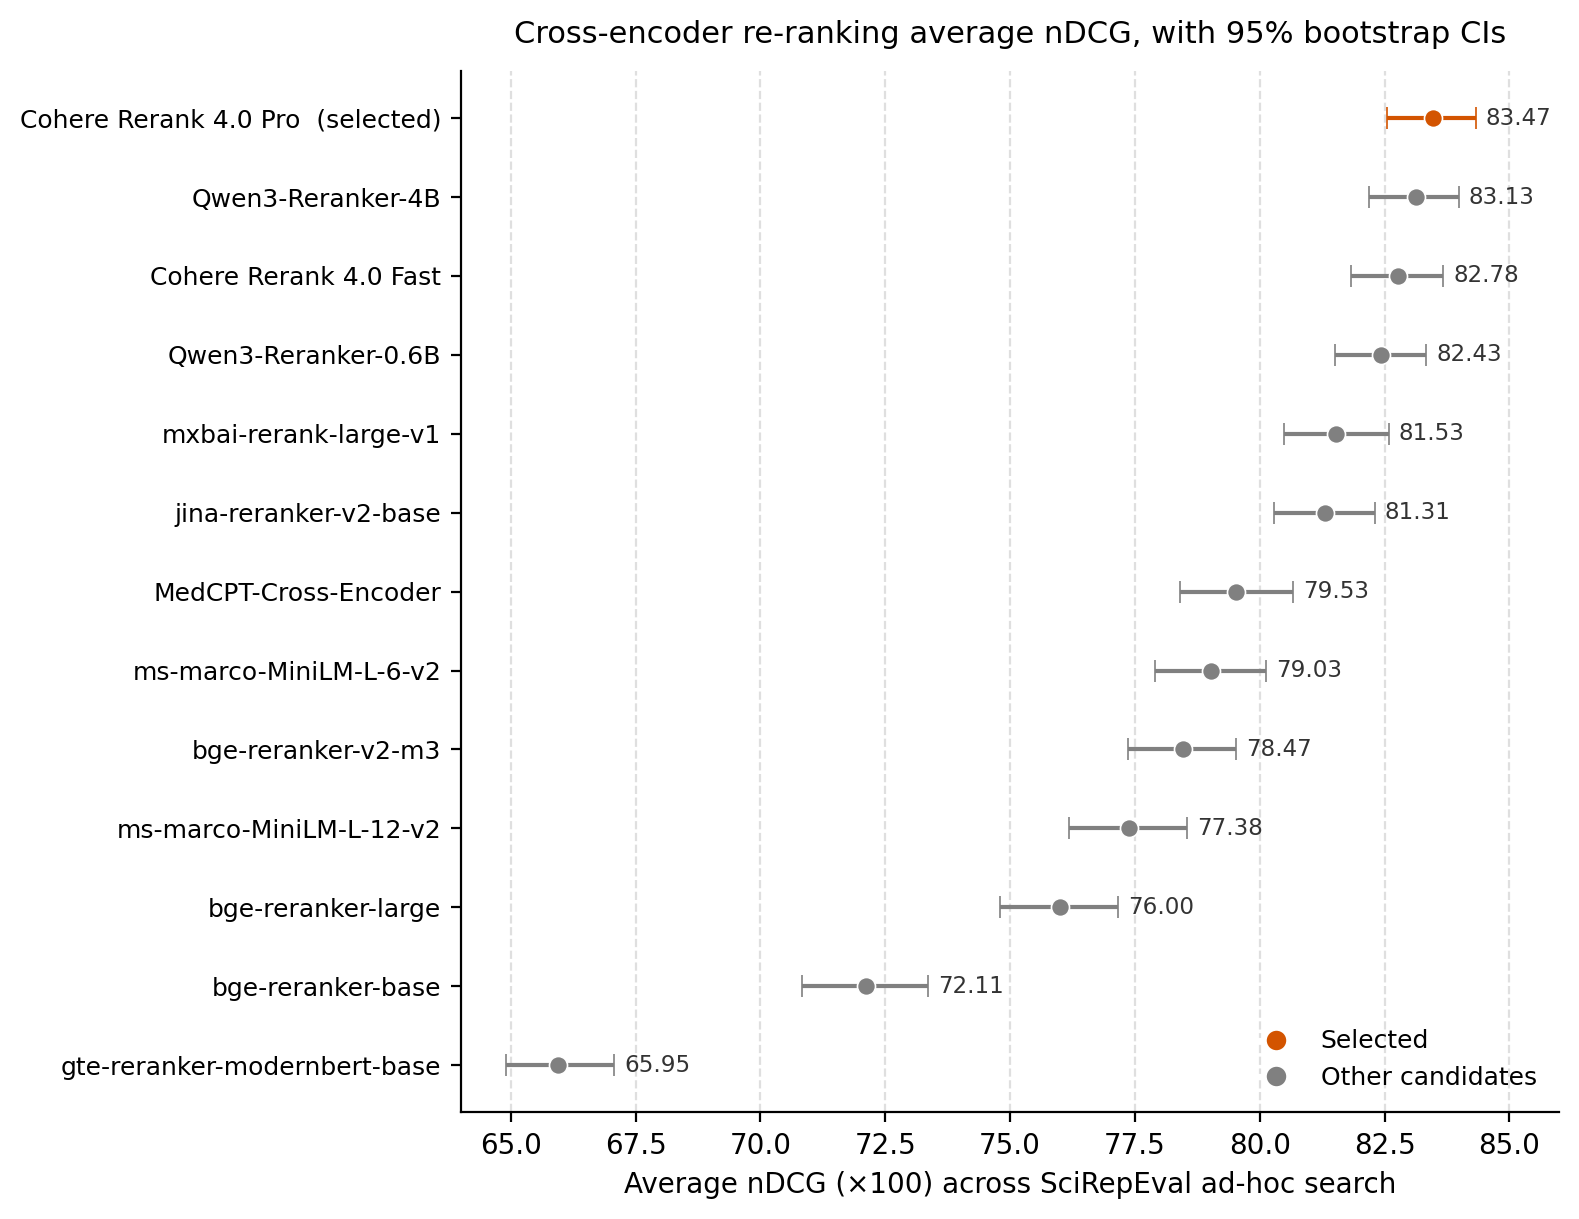
\includegraphics[width=\columnwidth]{images/data_and_results/crossencoder_average.png}
\caption{Cross-encoder re-ranking average nDCG across the three SciRepEval ad-hoc search tasks, with 95 percent bootstrap confidence intervals from 1000 resamples. The selected model is shown in orange.}
\label{fig:xenc-avg}
\end{figure}

\begin{figure}[t]
\centering
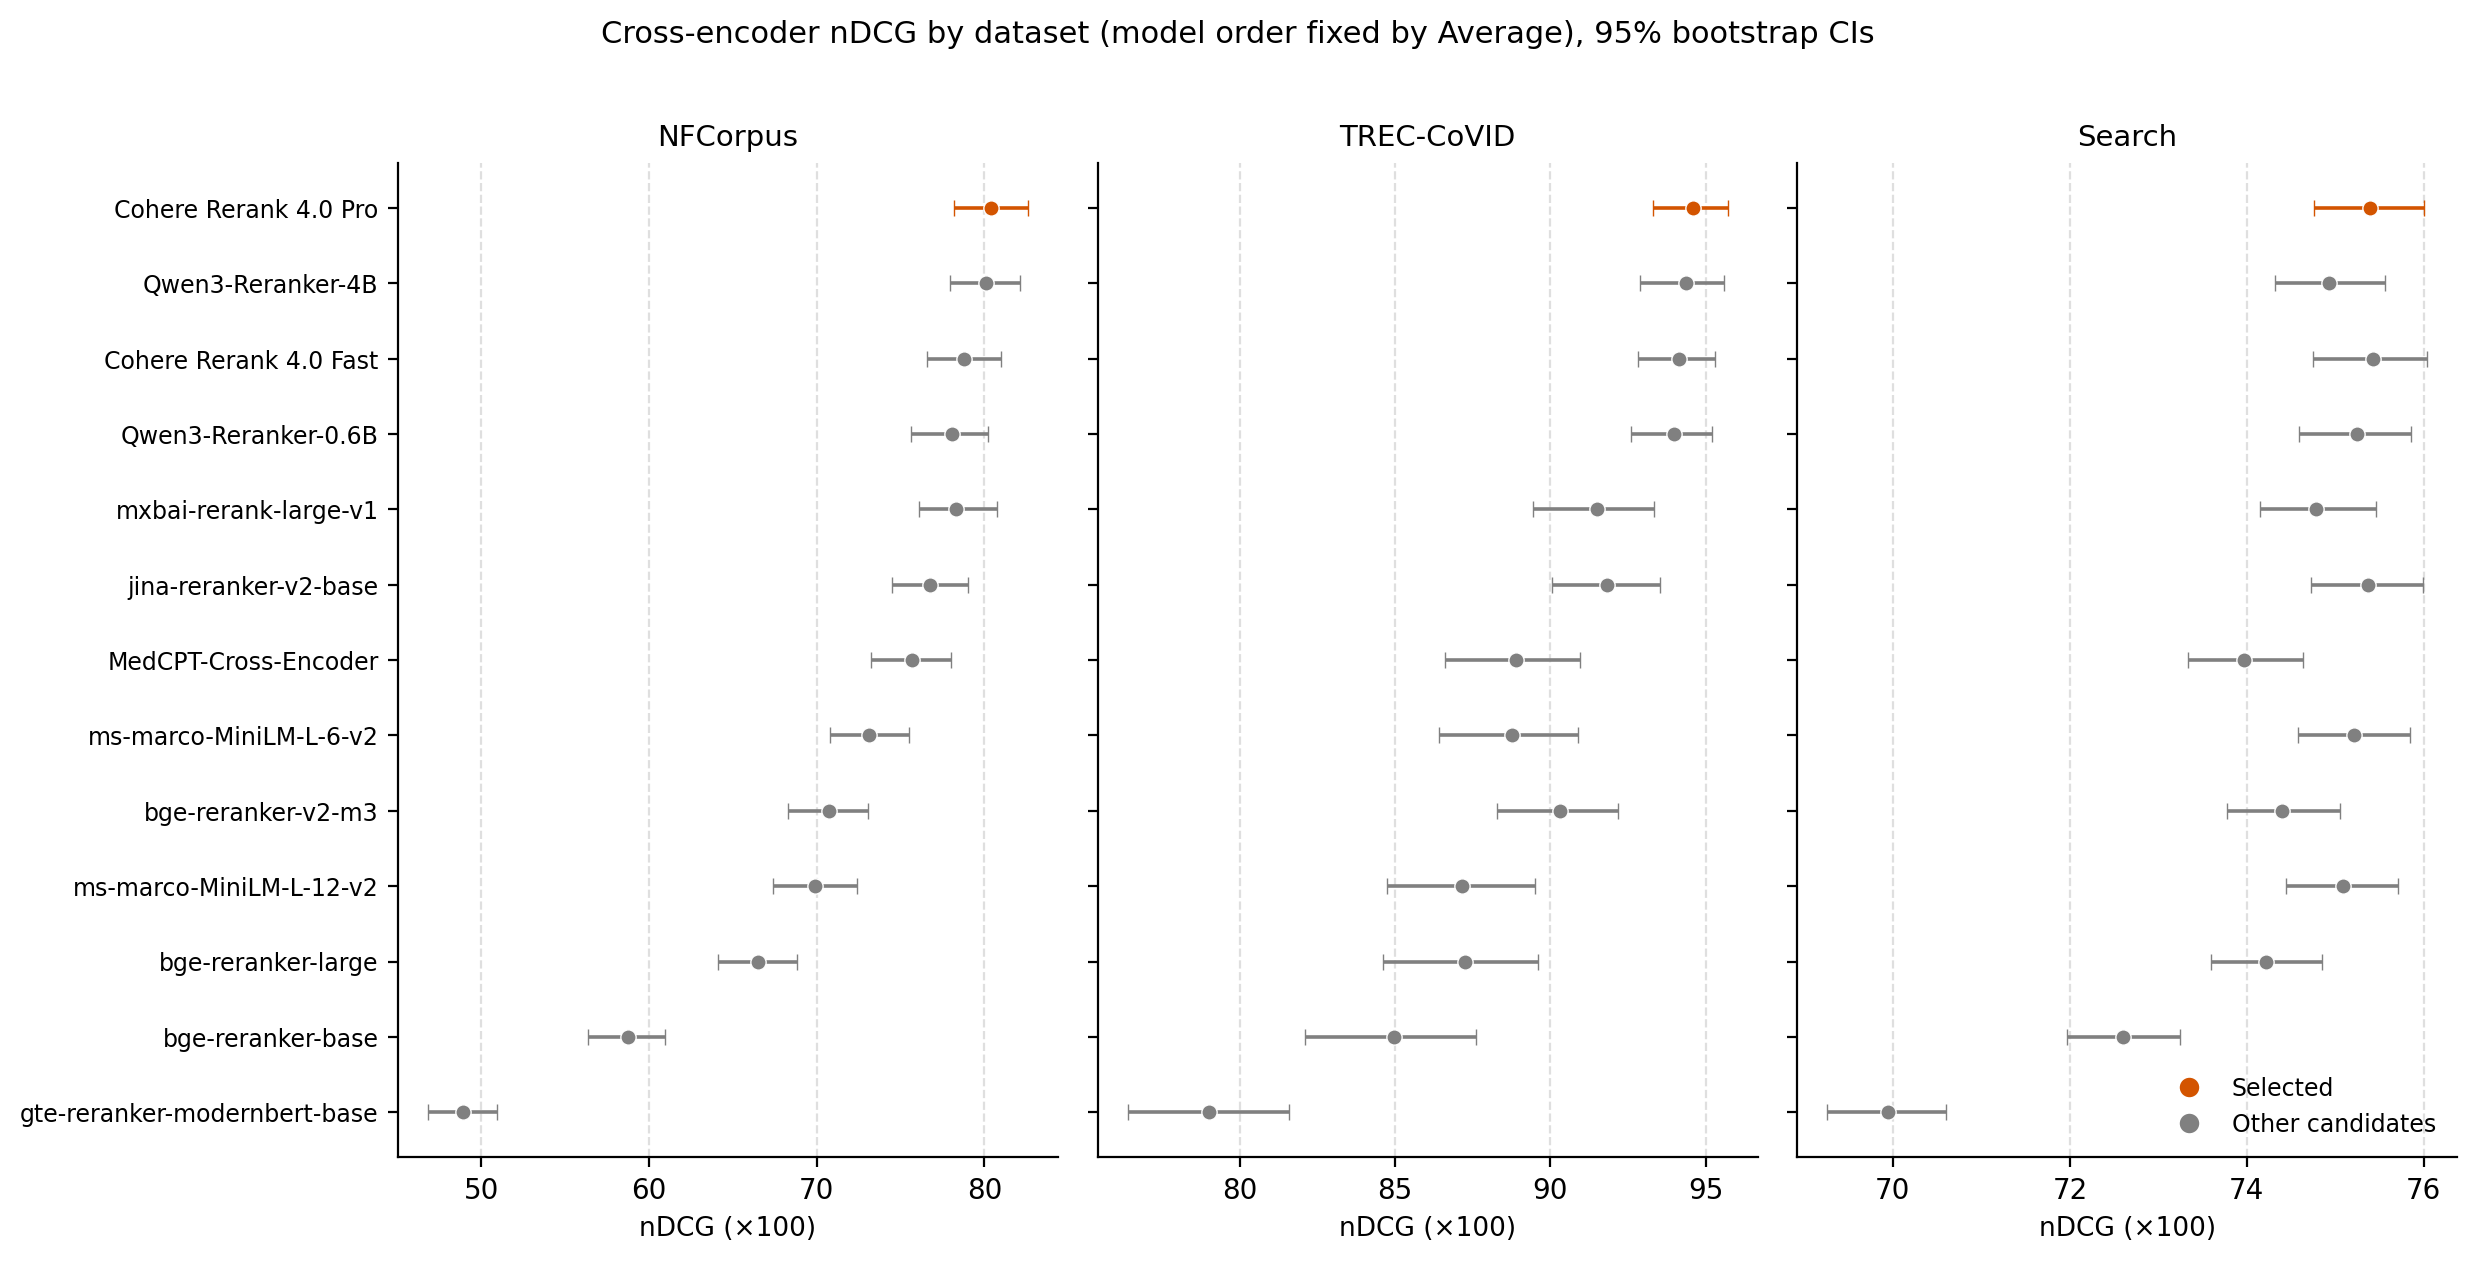
\includegraphics[width=\columnwidth]{images/data_and_results/crossencoder_by_dataset.png}
\caption{Cross-encoder nDCG on each SciRepEval ad-hoc search task, with models held in their Average order for comparison and 95 percent bootstrap confidence intervals. The selected model is shown in orange.}
\label{fig:xenc-pertask}
\end{figure}

Cohere Rerank 4.0 Pro was selected as the cross-encoder. The candidate rerankers were evaluated on the same three SciRepEval ad-hoc search tasks as the bi-encoder and under the same nDCG metric, scoring each model by the ranking it produces when it re-ranks the retrieved candidate pool. All scores are nDCG $\times$100 with 95 percent bootstrap intervals from 1000 resamples. The intervals are tight on Search, which has 2585 queries, and wide on TREC-CoVID, which has 50.

Table~\ref{tab:xenc-results} reports the full per-task and average scores, and Figure~\ref{fig:xenc-avg} plots each model's average with its interval. The selected model holds the highest average at 83.47. Its interval overlaps those of the next three models, Qwen3-Reranker-4B at 83.13, Cohere Rerank 4.0 Fast at 82.78, and Qwen3-Reranker-0.6B at 82.43, so these four form a statistical tie at the top. Within that group the strongest self-hostable model, Qwen3-Reranker-4B, is tied with the selected model. Below the leading four the field descends steadily through a long tail to gte-reranker-modernbert-base at 65.95, a spread of more than seventeen points from top to bottom.

The per-task view in Figure~\ref{fig:xenc-pertask} shows that almost all of this separation comes from NFCorpus, where the models spread across more than thirty points, from 80.42 at the top down to 48.88. Search behaves in the opposite way. Every reranker scores close to 75, since the small candidate pool the stage re-ranks leaves little room to reorder, so the task barely separates the models. TREC-CoVID falls between the two, with a high but noisy spread that reflects its fifty queries.

\begin{table*}[t]
\caption{Deployment characteristics of the candidate cross-encoders.}
\label{tab:xenc-deploy}
\centering
\footnotesize
\begin{tabular}{@{}p{4.5cm}llp{4.0cm}@{}}
\toprule
Model & Params (approx.) & Precision & Self-hostable \\
\midrule
Cohere Rerank 4.0 Pro & undisclosed & n/a & no (paid API) \\
Qwen3-Reranker-4B & $\sim$4 B & int8 & yes (Apache-2.0) \\
Cohere Rerank 4.0 Fast & undisclosed & n/a & no (paid API) \\
Qwen3-Reranker-0.6B & $\sim$0.6 B & fp16 & yes (Apache-2.0) \\
mxbai-rerank-large-v1 & $\sim$435 M & fp16 & yes \\
jina-reranker-v2-base & $\sim$278 M & fp16 & weights CC-BY-NC (non-commercial) \\
MedCPT-Cross-Encoder & $\sim$109 M & fp16 & yes \\
ms-marco-MiniLM-L-6-v2 & $\sim$22 M & fp16 & yes \\
bge-reranker-v2-m3 & $\sim$568 M & fp16 & yes \\
ms-marco-MiniLM-L-12-v2 & $\sim$33 M & fp16 & yes \\
bge-reranker-large & $\sim$560 M & fp16 & yes \\
bge-reranker-base & $\sim$278 M & fp16 & yes \\
gte-reranker-modernbert-base & $\sim$150 M & fp16 & yes \\
\bottomrule
\end{tabular}

\vspace{3pt}
\begin{minipage}{\linewidth}
\footnotesize\itshape
Unlike the bi-encoder, a reranker stores no vectors, so its cost is latency, which scales with parameter count, rather than memory, which is why the stage runs over only around 100 candidates. The Qwen3 rerankers are released under Apache-2.0, while the jina-reranker-v2 weights are CC-BY-NC-4.0 and so are non-commercial and not deployable in a commercial product. The remaining licences should be confirmed against the deployment terms before selection.
\end{minipage}
\end{table*}

Table~\ref{tab:xenc-deploy} records the deployment characteristics, namely approximate parameter count, precision, and whether the model is self-hostable along with its licence. Unlike the bi-encoder, a reranker stores no vectors, so its cost is latency rather than memory and scales with parameter count, which is the reason the stage runs over only around 100 candidates. The self-hostable options carry mixed licences, with the Qwen3 rerankers released under Apache-2.0 and the jina reranker under a non-commercial CC-BY-NC licence, while the selected model is served through a paid API.

% ----------------------------------------------------------------------------
\subsection{Embedding Quantisation}
% Placeholder. Results not yet available.
\textit{[Placeholder. Results comparing int8 against full-precision nDCG, and the resulting accuracy cost, to be added.]}

% ----------------------------------------------------------------------------
\subsection{System-Level Evaluation}
% Placeholder. Results not yet available.
\textit{[Placeholder. End-to-end results over a realistic query set with light relevance judgments to be added.]}   (or \include{...})
%
%  Requires in the preamble of main.tex:
%      \usepackage{booktabs}
%      \usepackage{graphicx}
%      \usepackage{array}      % only if you later add >{...} column types
%
%  Figures use placeholder paths under figures/ -- replace with your exports.
%  Tables and figures are referenced with \ref so numbering stays dynamic and
%  any table can be moved to an appendix without breaking the prose.
% ============================================================================

\section{Data and Results}

This section reports the result of each component benchmark from the validation design in Section~II-D, taking the components in turn.

% ----------------------------------------------------------------------------
\subsection{Keyword Generation}

\begin{table}[t]
\caption{KPBiomed keyword extraction, present and absent F1@5 with stemming. Models are ordered by present F1, and GPT-5.4-nano is the deployed model.}
\label{tab:kw-kpbiomed}
\centering
\footnotesize
\begin{tabular}{@{}lrr@{}}
\toprule
Model & Present F1@5 & Absent F1@5 \\
\midrule
\textbf{GPT-5.4-nano} & \textbf{30.86} & 1.95 \\
MultipartiteRank & 19.58 & 0.00 \\
TF-IDF & 18.56 & 0.04 \\
KeyBART & 17.40 & \textbf{2.07} \\
YAKE & 16.79 & 0.02 \\
KBIR-inspec & 16.36 & 0.01 \\
KeyBERT-MiniLM & 8.52 & 0.04 \\
TextRank & 5.11 & 0.00 \\
\bottomrule
\end{tabular}
\end{table}

\begin{figure*}[t]
\centering
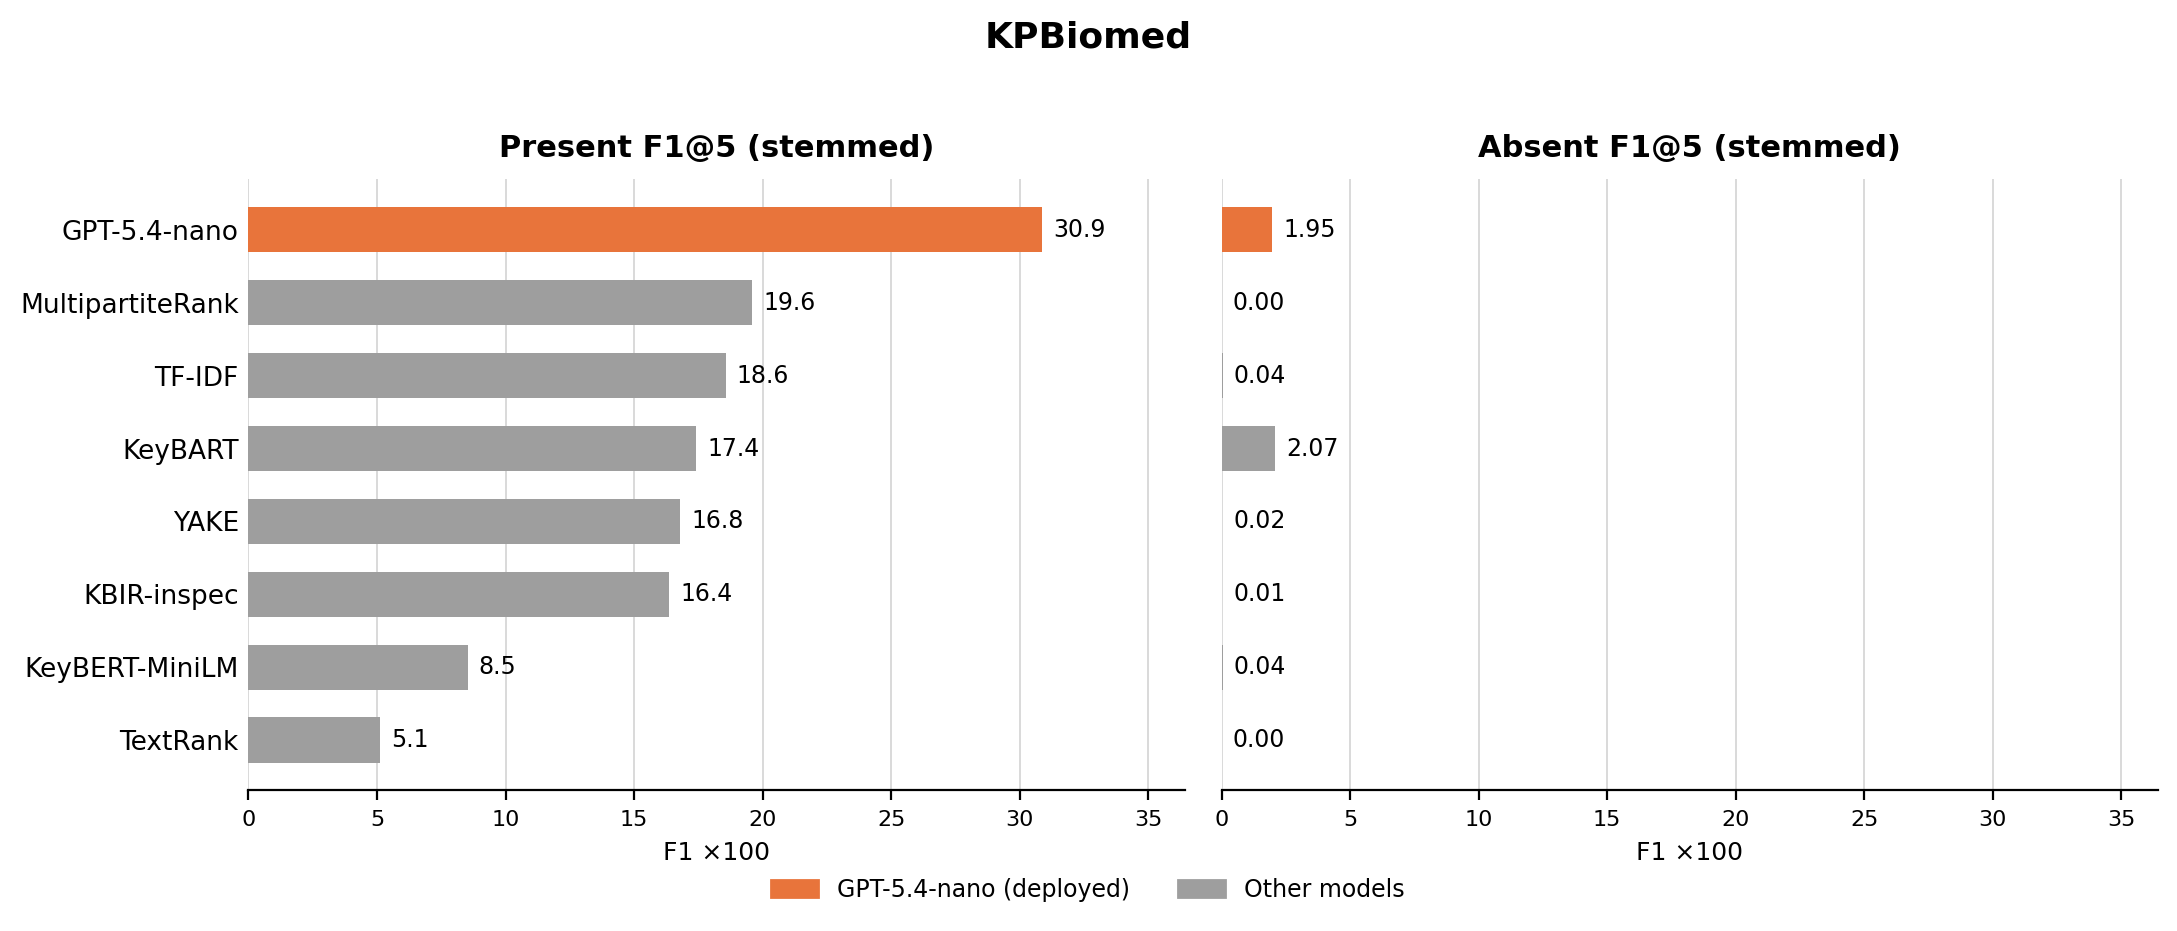
\includegraphics[width=\textwidth]{images/data_and_results/keyword_kpbiomed.png}
\caption{KPBiomed keyword extraction, present and absent F1@5 by model with stemming. The deployed model GPT-5.4-nano is shown in orange and the remaining baselines in grey.}
\label{fig:kw-kpbiomed}
\end{figure*}

\begin{table}[t]
\caption{OAGKX keyword extraction, present and absent F1@5 with stemming. Models are ordered by present F1, and GPT-5.4-nano is the deployed model.}
\label{tab:kw-oagkx}
\centering
\footnotesize
\begin{tabular}{@{}lrr@{}}
\toprule
Model & Present F1@5 & Absent F1@5 \\
\midrule
KeyBART & \textbf{28.42} & \textbf{5.09} \\
\textbf{GPT-5.4-nano} & 26.49 & 1.77 \\
KBIR-inspec & 20.16 & 0.05 \\
MultipartiteRank & 18.83 & 0.00 \\
TF-IDF & 15.55 & 0.03 \\
KeyBERT-MiniLM & 12.04 & 0.04 \\
TextRank & 11.15 & 0.02 \\
YAKE & 8.85 & 0.00 \\
\bottomrule
\end{tabular}
\end{table}

\begin{figure*}[t]
\centering
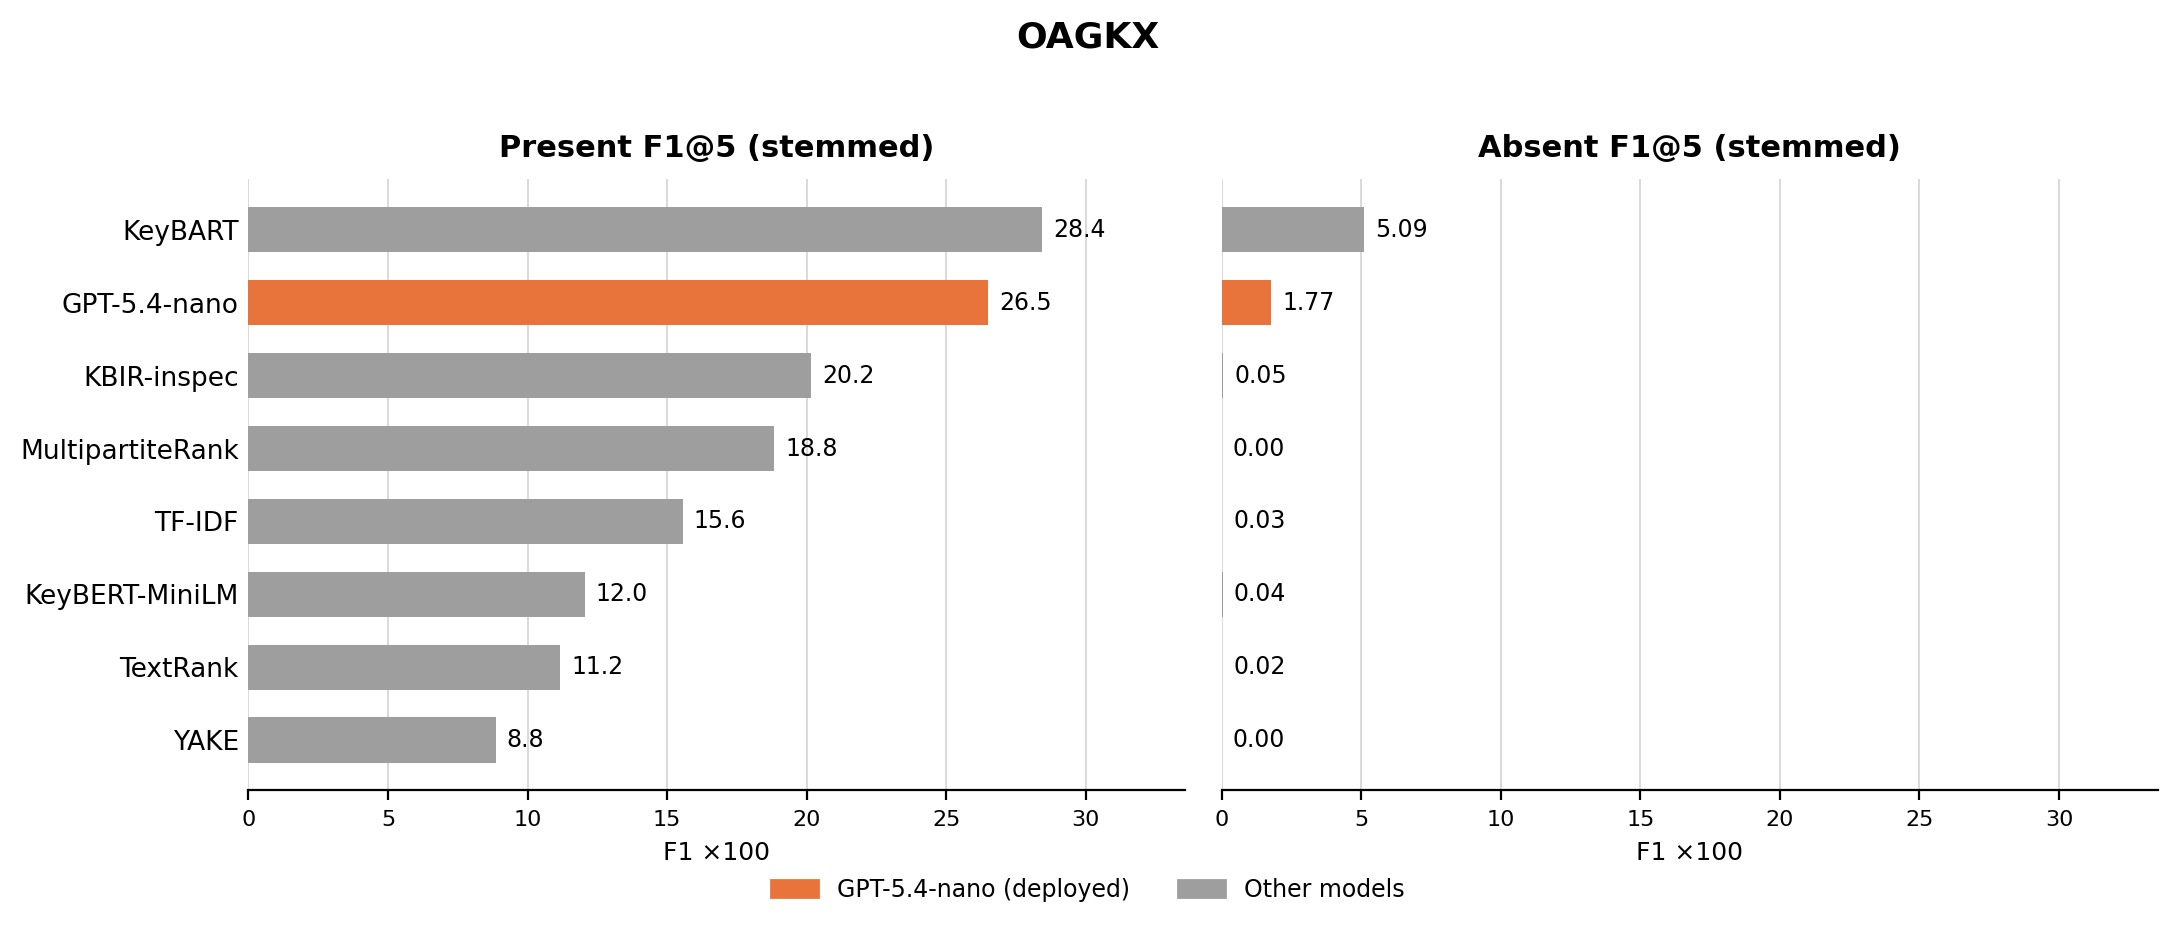
\includegraphics[width=\textwidth]{images/data_and_results/keyword_oagkx.png}
\caption{OAGKX keyword extraction, present and absent F1@5 by model with stemming. The deployed model GPT-5.4-nano is shown in orange and the remaining baselines in grey.}
\label{fig:kw-oagkx}
\end{figure*}

\begin{table}[t]
\caption{PubMedAKE keyword extraction, present and absent F1@5 with stemming. Models are ordered by present F1, and GPT-5.4-nano is the deployed model.}
\label{tab:kw-pubmedake}
\centering
\footnotesize
\begin{tabular}{@{}lrr@{}}
\toprule
Model & Present F1@5 & Absent F1@5 \\
\midrule
\textbf{GPT-5.4-nano} & \textbf{36.44} & \textbf{1.30} \\
TF-IDF & 24.06 & 0.03 \\
MultipartiteRank & 23.06 & 0.00 \\
KBIR-inspec & 19.36 & 0.01 \\
KeyBART & 18.41 & 1.29 \\
YAKE & 12.92 & 0.01 \\
KeyBERT-MiniLM & 6.78 & 0.01 \\
TextRank & 4.68 & 0.00 \\
\bottomrule
\end{tabular}
\end{table}

\begin{figure*}[t]
\centering
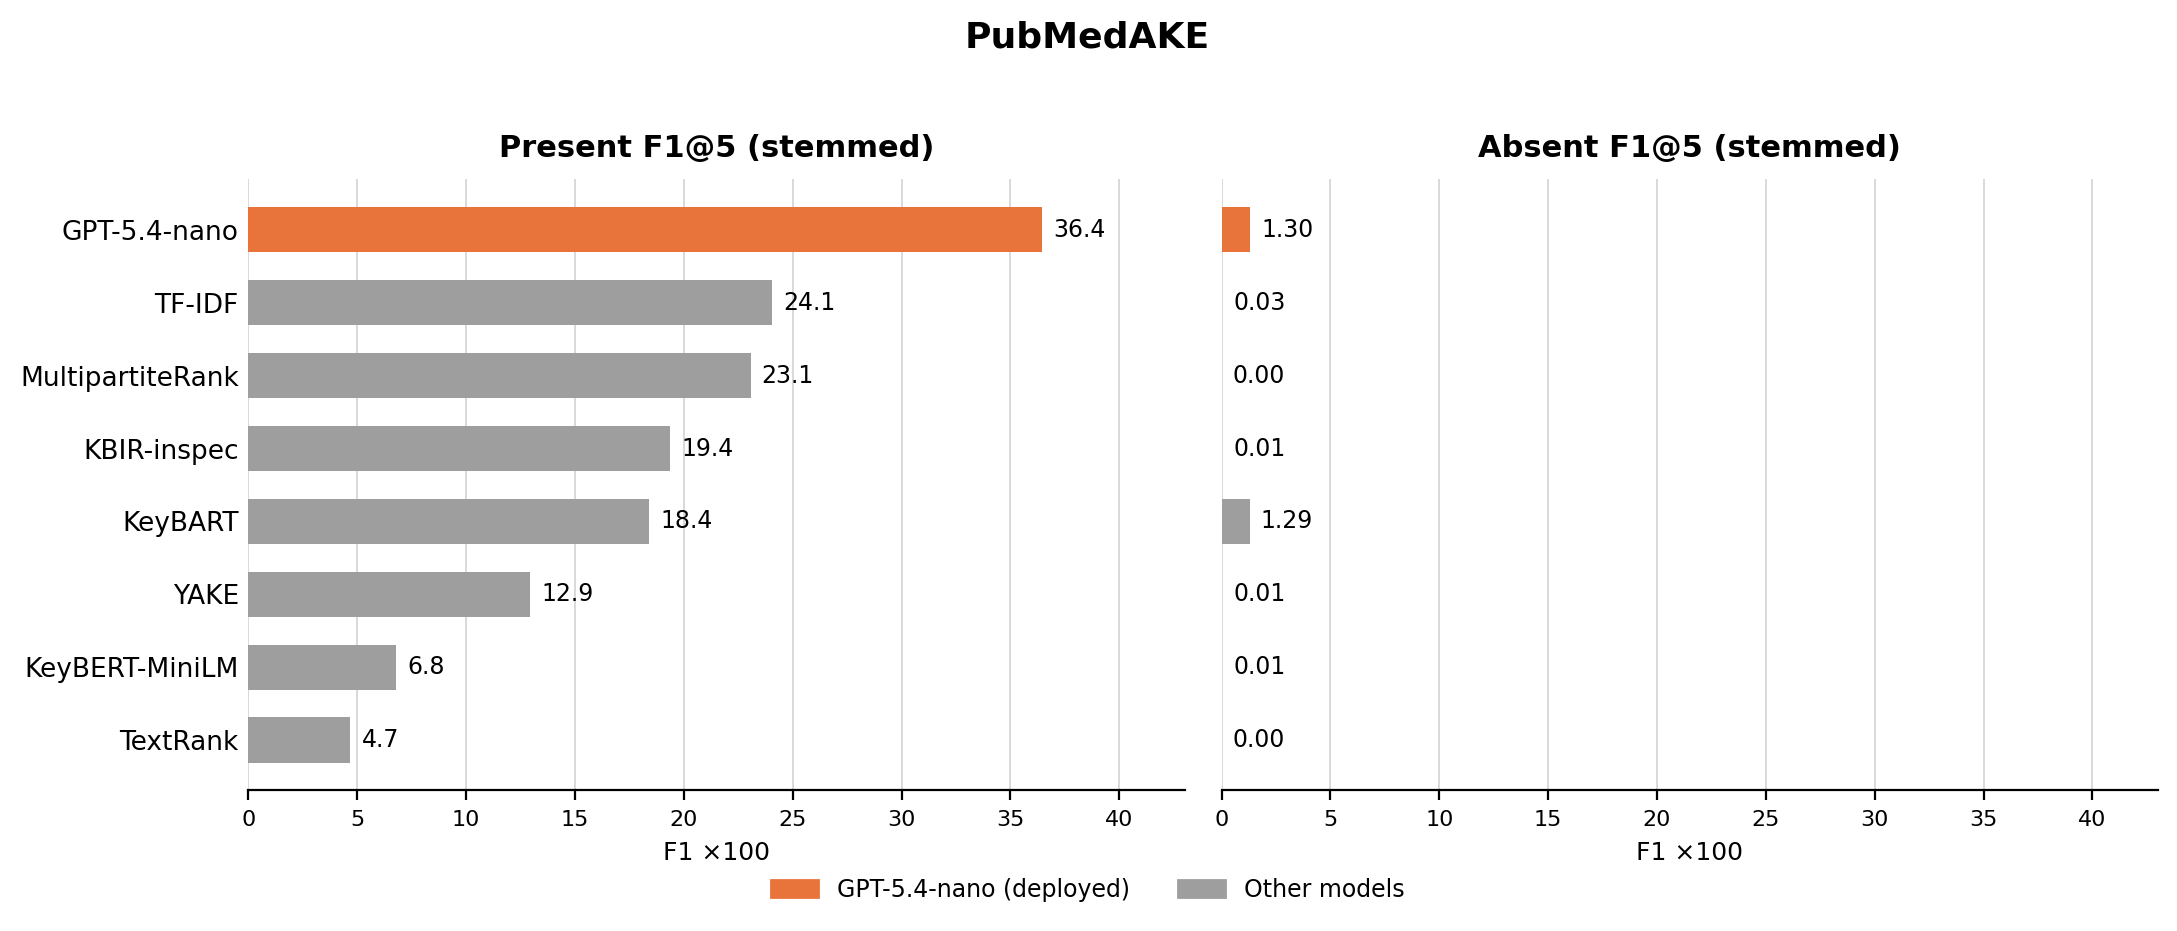
\includegraphics[width=\textwidth]{images/data_and_results/keyword_pubmedake.png}
\caption{PubMedAKE keyword extraction, present and absent F1@5 by model with stemming. The deployed model GPT-5.4-nano is shown in orange and the remaining baselines in grey.}
\label{fig:kw-pubmedake}
\end{figure*}

GPT-5.4-nano was benchmarked for keyword generation against a set of statistical and neural baselines on KPBiomed, OAGKX, and PubMedAKE. Tables~\ref{tab:kw-kpbiomed} to~\ref{tab:kw-pubmedake} report the results for each dataset in turn. Throughout, present (extractive) keyphrases, which occur verbatim in the source text, are distinguished from absent (abstractive) keyphrases, which do not and so must be generated. Matches are scored by F1 at five with light stemming, so that a keyphrase and its stem count as a match while a different word of the same meaning does not.

On the present keyphrase tasks, GPT-5.4-nano records the highest score on KPBiomed and PubMedAKE and the second highest on OAGKX, where KeyBART leads. Its margin is widest on PubMedAKE, at 36.44 against a next-best of 24.06.

On the absent keyphrase tasks, which a model can only score on by producing keyphrases that do not occur in the source text, GPT-5.4-nano scores in the low single digits, from 1.30 on PubMedAKE to 1.95 on KPBiomed. These non-zero scores indicate that the model generates a small portion of its keyphrases rather than extracting all of them. The other generative baseline, KeyBART, behaves similarly and records the highest absent score on KPBiomed and OAGKX. The statistical extractors such as TF-IDF, YAKE, TextRank, and MultipartiteRank remain near zero here, since they return only spans found in the source text and so do not generate at all.

\begin{table}[t]
\caption{Keyword extraction stability for GPT-5.4-nano over three runs on a 2000-document sample.}
\label{tab:kw-stability}
\centering
\footnotesize
\begin{tabular}{@{}p{0.66\columnwidth}r@{}}
\toprule
Quantity & Value \\
\midrule
Set-level Jaccard across runs & 0.73 \\
Present-F1 run-to-run std & $\pm$0.07 \\
Deterministic baselines (TF-IDF, YAKE, TextRank, MultipartiteRank, KeyBERT, KBIR) & 1.00 \\
\bottomrule
\end{tabular}
\end{table}

Table~\ref{tab:kw-stability} reports a reproducibility check for GPT-5.4-nano over three runs on a 2000-document sample. The set-level Jaccard similarity across runs is 0.73, meaning that for a given document around 73 percent of the combined set of keyphrases from any two runs is shared by both, equivalent to roughly one in six keyphrases changing between runs. The model is therefore largely repeatable but not deterministic, unlike the baselines, which are reproducible by construction. The effect on measured performance is negligible, with a run-to-run present-F1 standard deviation of 0.07. The same sample also reproduces the full-split figures to within roughly a tenth of a point, confirming that the smaller stability sample does not shift the headline results.

% ----------------------------------------------------------------------------
\subsection{IR Extraction}

\begin{table*}[t]
\caption{Natural-language-to-IR accuracy by model. Joint IR accuracy counts a query as correct when both its entities and its boolean expression are correct under exact matching, reported in the as-deployed or best configuration for each model.}
\label{tab:ir-accuracy}
\centering
\footnotesize
\begin{tabular}{@{}lllcc@{}}
\toprule
Model & Host & Configuration & IR accuracy & 95\% CI \\
\midrule
\textbf{gpt-5.4-nano} & Azure & default, 0 reasoning tok & \textbf{0.937}$^{\dagger}$ & [0.897, 0.983] \\
gpt-5-mini & Azure & default, 384 reasoning tok & 0.931 & [0.879, 0.974] \\
qwen3:8b & Local (Q4) & single-shot & 0.802 & [0.733, 0.871] \\
qwen3:4b & Local (Q4) & thinking$^{\ddagger}$ & 0.784 & [0.707, 0.862] \\
qwen2.5:3b & Local (Q4) & non-reasoning & 0.207 & [0.138, 0.284] \\
phi4-mini & Local (Q4) & non-reasoning & 0.052 & [0.017, 0.095] \\
llama3.2:3b & Local (Q4) & non-reasoning & 0.026 & [0.000, 0.060] \\
\bottomrule
\end{tabular}

\vspace{3pt}
\begin{minipage}{\linewidth}
\footnotesize\itshape
Confidence intervals are 95 percent bootstrap over 1000 iterations. Cross-model gaps that fall within these intervals are treated as ties, and bold marks the deployed model. The dagger denotes a three-run mean, whose single-run range is 0.914 to 0.940, with temperature zero returning a byte-identical output on 96.6 percent of queries (Table~\ref{tab:ir-stability}). The double dagger denotes qwen3:4b, whose single-shot configuration produced degenerate empty output, so its thinking configuration is its only usable score.
\end{minipage}
\end{table*}

\begin{figure}[t]
\centering
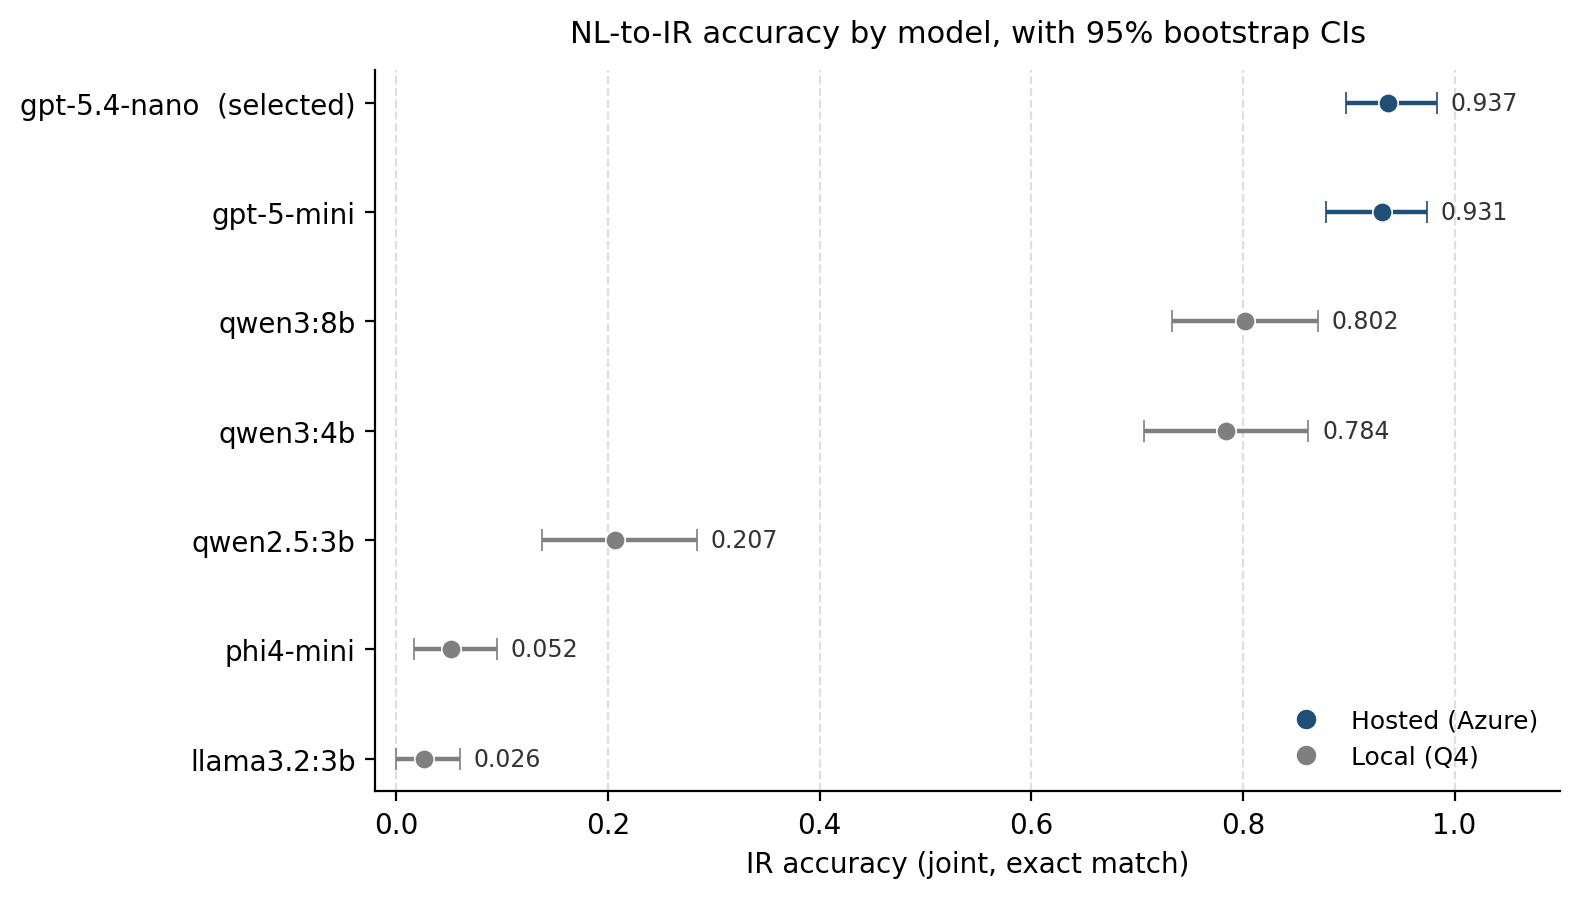
\includegraphics[width=\columnwidth]{images/data_and_results/ir_accuracy_ci.png}
\caption{Natural-language-to-IR joint accuracy by model on the hand-built gold set, with 95 percent bootstrap confidence intervals from 1000 resamples.}
\label{fig:ir-accuracy}
\end{figure}

GPT-5.4-nano was benchmarked for natural-language-to-IR extraction against a set of hosted and local models on a hand-built gold set of queries paired with their correct intermediate representations. The set was constructed to exercise every entity type the system supports across a range of boolean structures, from single topics through to bracketed combinations of AND, OR, and NOT, so that performance on it reflects the input and output behaviour the system actually requires. The headline measure, IR accuracy, is the joint figure reported in Table~\ref{tab:ir-accuracy}, counting a query as correct only when both its extracted entities and its boolean expression are correct under exact matching.

Figure~\ref{fig:ir-accuracy} plots each model's accuracy with its 95 percent bootstrap interval. The two hosted models lead the benchmark by a clear margin, with GPT-5.4-nano highest at an IR accuracy of 0.937 and GPT-5-mini close behind at 0.931. Both hosted intervals clear those of every local model without overlap, placing the hosted advantage beyond sampling noise, while the two overlap each other and are statistically indistinguishable. Among the local models, the two strongest (qwen3:8b and qwen3:4b) reach around 0.80, and the three smaller models fall away sharply to 0.207, 0.052, and 0.026, near the floor of the task.

\begin{table}[t]
\caption{Effect of reasoning on IR accuracy.}
\label{tab:ir-reasoning}
\centering
\footnotesize
\begin{tabular}{@{}lccc@{}}
\toprule
Model & Reasoning off & Reasoning on & $\Delta$ \\
\midrule
gpt-5.4-nano & 0.914 & 0.922 & +0.008 \\
gpt-5-mini & \textbf{0.750} & \textbf{0.940} & \textbf{+0.190} \\
\bottomrule
\end{tabular}

\vspace{3pt}
\begin{minipage}{\linewidth}
\footnotesize\itshape
Reasoning is controlled through the Azure \texttt{reasoning\_effort} setting with tokens accounted. Reasoning on used approximately 246 tokens per query for gpt-5.4-nano and 896 for gpt-5-mini, while reasoning off used none. Reasoning lifts the weaker model in each tier, while the stronger one is already at its ceiling.
\end{minipage}
\end{table}

Table~\ref{tab:ir-reasoning} isolates the effect of reasoning on the two GPT models. GPT-5.4-nano gains almost nothing from it, moving from 0.914 without reasoning to 0.922 with around 246 reasoning tokens, a difference of 0.008, and so reaches its accuracy in a single pass with no reasoning budget. GPT-5-mini behaves differently, scoring only 0.750 without reasoning and rising to 0.940 once reasoning is enabled, at a cost of around 896 reasoning tokens per query. The stronger model is already at its ceiling unaided, whereas the weaker one becomes competitive only by spending a substantial token budget.

\begin{table}[t]
\caption{Deployed model, metric decomposition in the default-effort configuration.}
\label{tab:ir-decomp}
\centering
\footnotesize
\begin{tabular}{@{}lcc@{}}
\toprule
Metric & Value & 95\% CI \\
\midrule
IR accuracy (joint) & 0.937 & [0.897, 0.983] \\
Entity F1 (micro) & 0.984 & [0.969, 0.995] \\
Entity F1 (macro) & 0.982 & [0.967, 0.994] \\
Expression equivalence & 0.931 & [0.888, 0.974] \\
Expression graded & 0.985 & [0.974, 0.995] \\
\bottomrule
\end{tabular}

\vspace{3pt}
\begin{minipage}{\linewidth}
\footnotesize\itshape
Joint accuracy is bounded by expression equivalence, since entity extraction almost never fails on its own.
\end{minipage}
\end{table}

\begin{table}[t]
\caption{Deployed model, accuracy by stratum, ordered hardest first.}
\label{tab:ir-stratum}
\centering
\footnotesize
\begin{tabular}{@{}lrrr@{}}
\toprule
Stratum & $n$ & IR accuracy & failures \\
\midrule
\texttt{filter\_distractor} & 10 & 0.700 & 3 \\
\texttt{multi\_negation} & 10 & 0.800 & 2 \\
\texttt{deep\_nested} & 12 & 0.833 & 2 \\
\texttt{hard\_typing} & 12 & 0.917 & 1 \\
\texttt{single\_concept} & 6 & 1.000 & 0 \\
\texttt{multi\_concept} & 12 & 1.000 & 0 \\
\texttt{exclusion} & 12 & 1.000 & 0 \\
\texttt{nested} & 12 & 1.000 & 0 \\
\texttt{mixed\_entity} & 16 & 1.000 & 0 \\
\texttt{review\_style} & 14 & 1.000 & 0 \\
\bottomrule
\end{tabular}

\vspace{3pt}
\begin{minipage}{\linewidth}
\footnotesize\itshape
The count $n$ is small per stratum, at sixteen or fewer, so the failure counts are a more reliable read than the rate, and the per-stratum 95 percent intervals are wide, for example \texttt{filter\_distractor} at 0.700 is seven of ten.
\end{minipage}
\end{table}

Tables~\ref{tab:ir-decomp} and~\ref{tab:ir-stratum} decompose the chosen model's performance, which is strong across both components and most query types. By component, entity extraction is near-perfect, with a micro F1 of 0.984 and a macro F1 of 0.982, while expression equivalence is lower at 0.931 (a graded variant that credits partially correct expressions reaches 0.985). The joint IR accuracy of 0.937 is therefore bounded by the expression score, since entity extraction almost never fails on its own. By query type, the model is perfect on six of the ten strata, covering single and multiple concepts, exclusions, nesting, mixed entities, and review-style queries. Its errors concentrate in the remaining four. The largest source is \texttt{filter\_distractor}, where three of ten queries fail because the model miscategorises a filter term such as a year or citation bound as a searchable entity. The rest fall on the structurally hardest queries, with two of ten failing on multiple negations, two of twelve on deep nesting, and one of twelve on hard typing. Per-stratum counts are small, at sixteen queries or fewer, so the failure counts are a more reliable read than the rates.

\begin{table}[t]
\caption{Stability of the deployed model over three runs.}
\label{tab:ir-stability}
\centering
\footnotesize
\begin{tabular}{@{}p{0.46\columnwidth}cc@{}}
\toprule
Metric & temp 0 & temp 0.7 \\
\midrule
IR identical across all 3 runs & 0.966 & 0.957 \\
Run-to-run IR-accuracy std & 0.004 & 0.004 \\
Majority-vote@3 vs single run & 0.931 vs 0.940 & 0.940 vs 0.940 \\
\bottomrule
\end{tabular}

\vspace{3pt}
\begin{minipage}{\linewidth}
\footnotesize\itshape
Temperature zero is highly but not perfectly deterministic, and majority voting adds nothing.
\end{minipage}
\end{table}

Table~\ref{tab:ir-stability} reports a stability check over three runs. Although GPT-5.4-nano is not deterministic, at temperature zero it returns an identical IR on 96.6 percent of queries, with a run-to-run accuracy standard deviation of 0.004. Aggregating three runs by majority vote changes nothing, at 0.931 against 0.940 for a single run, so the three-run mean of 0.937 reported in Table~\ref{tab:ir-accuracy} is used throughout.

% ----------------------------------------------------------------------------
\subsection{Dense Bi-encoder Retrieval}

\begin{table*}[t]
\caption{Dense bi-encoder retrieval on SciRepEval ad-hoc search, nDCG $\times$100 with 95 percent bootstrap confidence intervals.}
\label{tab:bienc-results}
\centering
\scriptsize
\setlength{\tabcolsep}{4pt}
\begin{tabular}{@{}p{3.0cm}llll@{}}
\toprule
Model & NFCorpus & TREC-CoVID & Search & Average \\
\midrule
Qwen3-Embedding-4B (int8) & \textbf{80.02 [77.75, 82.17]} & \textbf{94.28 [92.96, 95.43]} & 75.54 [74.93, 76.17] & \textbf{83.28 [82.35, 84.19]} \\
EmbeddingGemma-300M & 79.13 [76.84, 81.29] & 92.45 [90.68, 94.03] & 75.32 [74.66, 75.93] & 82.30 [81.32, 83.31] \\
Qwen3-Embedding-0.6B & 77.94 [75.75, 80.22] & 93.90 [92.52, 95.10] & 75.03 [74.41, 75.65] & 82.29 [81.32, 83.25] \\
text-embedding-3-small (existing) & 78.78 [76.61, 81.05] & 92.38 [90.58, 93.96] & 75.14 [74.52, 75.74] & 82.10 [81.08, 83.05] \\
mxbai-embed-large-v1 & 79.37 [77.19, 81.72] & 91.77 [90.02, 93.25] & 74.92 [74.29, 75.56] & 82.02 [81.06, 82.96] \\
SPECTER2-adhoc-query & 70.46 [68.01, 72.97] & 90.08 [87.84, 92.13] & \textbf{78.22 [77.60, 78.86]} & 79.59 [78.46, 80.71] \\
BGE-M3 & 74.05 [71.72, 76.35] & 89.21 [87.08, 91.16] & 74.82 [74.20, 75.46] & 79.36 [78.29, 80.42] \\
SPECTER2-base (existing) & 72.03 [69.60, 74.54] & 89.46 [86.99, 91.58] & 73.76 [73.12, 74.41] & 78.42 [77.27, 79.58] \\
\bottomrule
\end{tabular}

\vspace{3pt}
\begin{minipage}{\linewidth}
\footnotesize\itshape
The metric is SciRepEval ad-hoc-search full-ranking nDCG over a per-query candidate pool, not BEIR full-corpus nDCG@10. Confidence intervals are 95 percent bootstrap [lo, hi] over 1000 iterations with seed 42, and bold marks the best point estimate per column. On Average the top five models' intervals overlap, a statistical tie, and SPECTER2-adhoc-query's Search lead is the one between-model gap whose interval clears the general models.
\end{minipage}
\end{table*}

\begin{figure}[t]
\centering
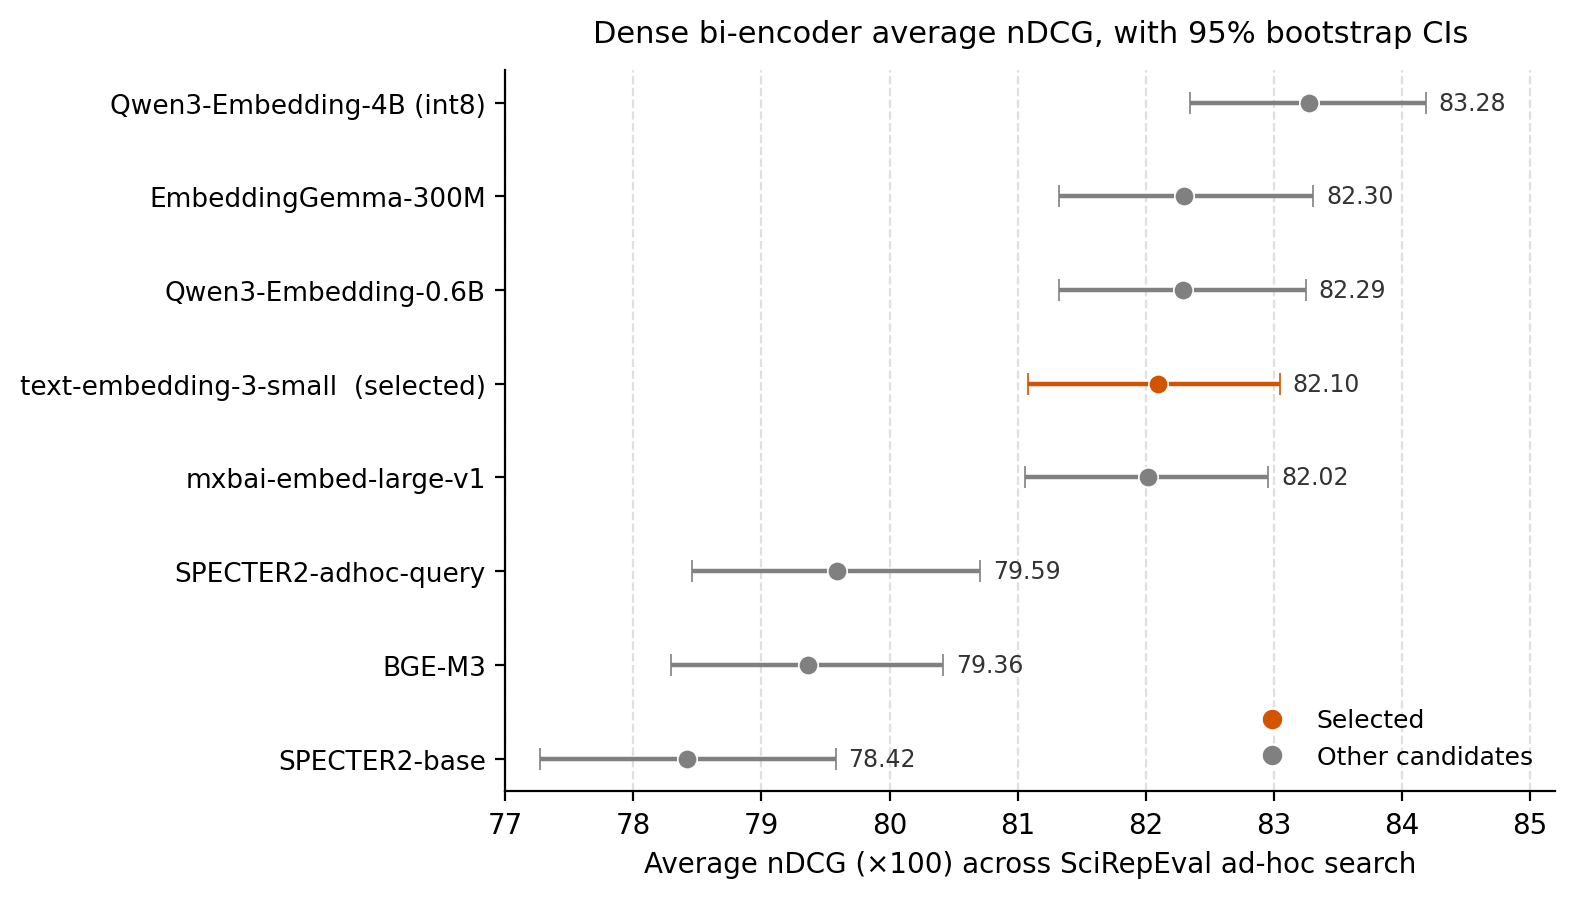
\includegraphics[width=\columnwidth]{images/data_and_results/biencoder_average.png}
\caption{Dense bi-encoder average nDCG across the three SciRepEval ad-hoc search tasks, with 95 percent bootstrap confidence intervals from 1000 resamples. The selected model is shown in orange.}
\label{fig:bienc-avg}
\end{figure}

\begin{figure}[t]
\centering
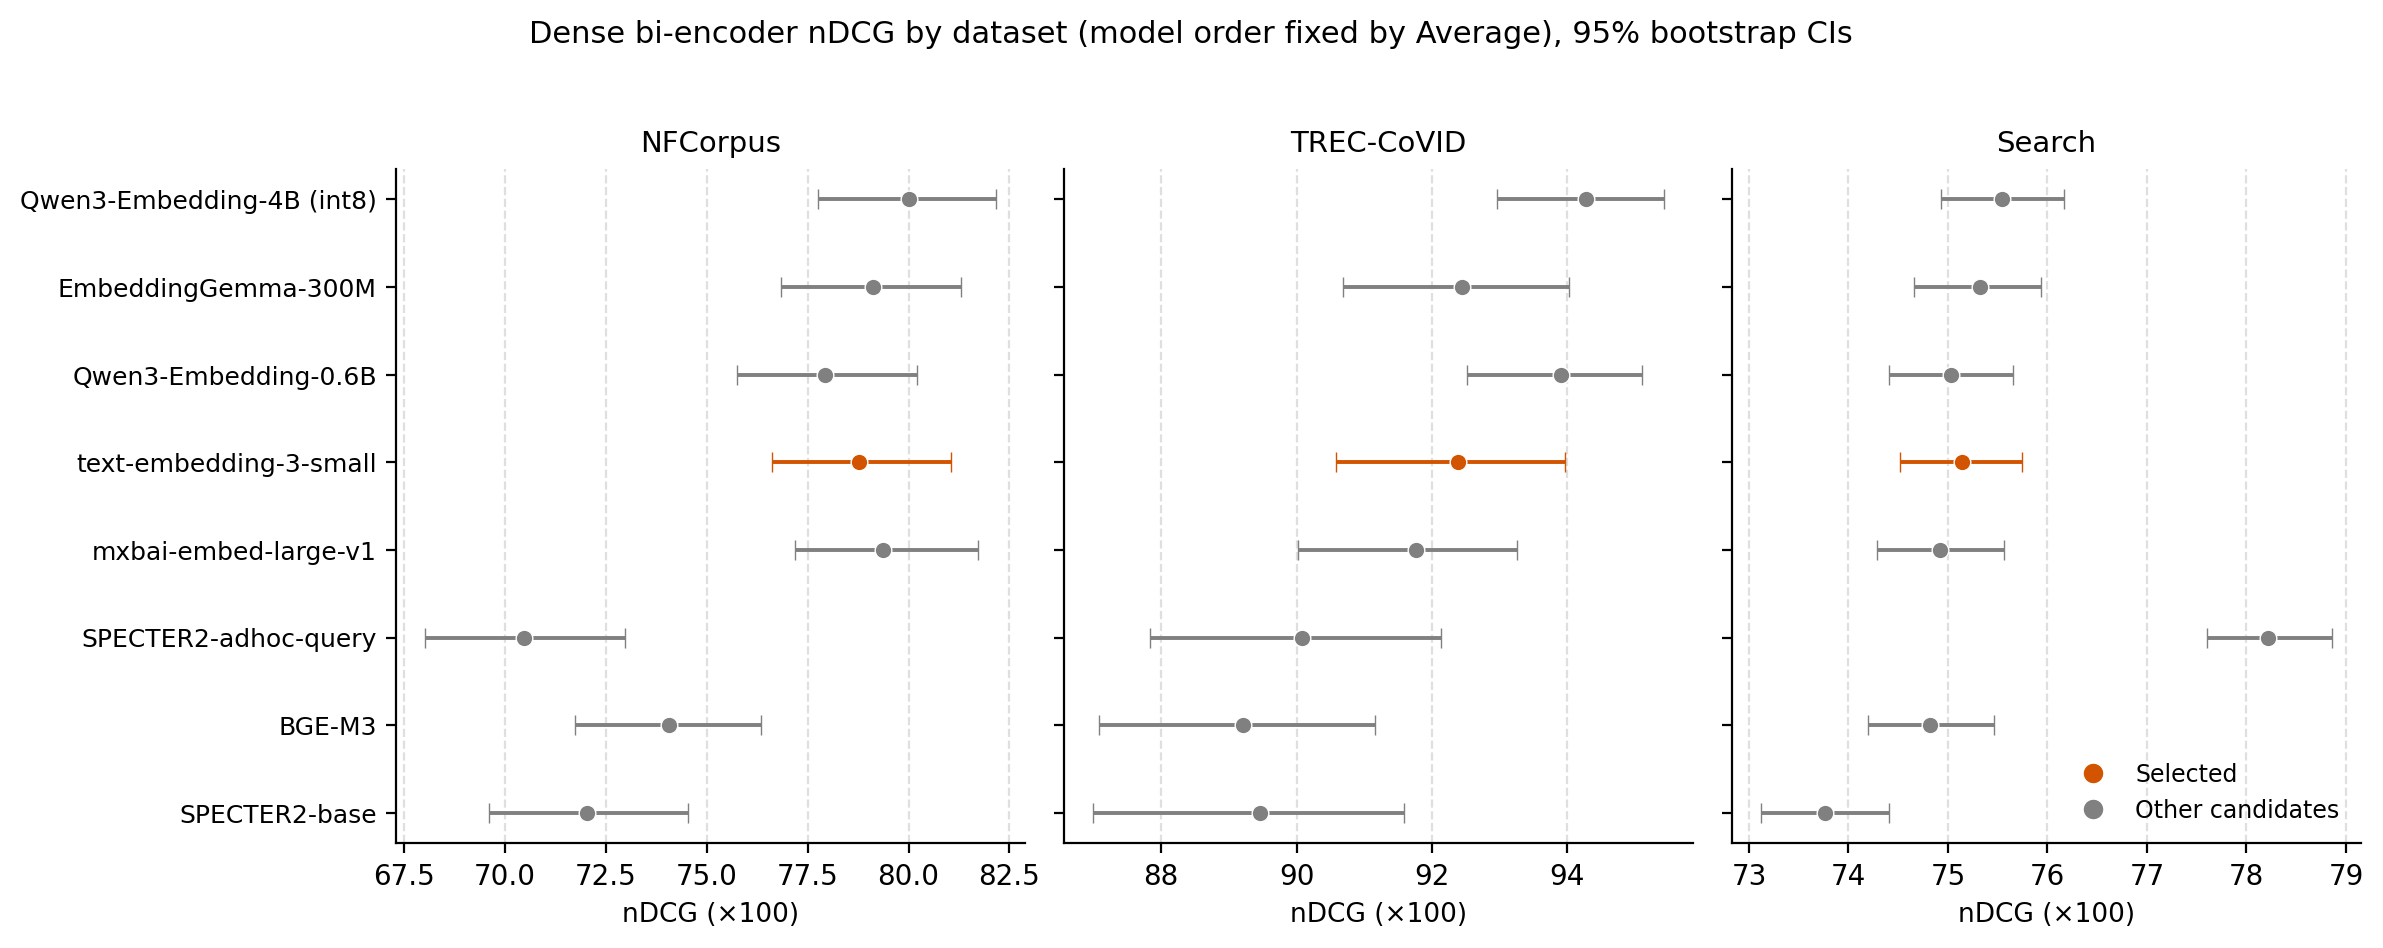
\includegraphics[width=\columnwidth]{images/data_and_results/biencoder_by_dataset.png}
\caption{Dense bi-encoder nDCG on each SciRepEval ad-hoc search task, with models held in their Average order for comparison and 95 percent bootstrap confidence intervals. The selected model is shown in orange.}
\label{fig:bienc-pertask}
\end{figure}

text-embedding-3-small was selected as the dense bi-encoder. The candidate models were evaluated on the three ad-hoc search tasks of SciRepEval, namely NFCorpus, TREC-CoVID, and Search, scored by nDCG. The figure reported is SciRepEval full-ranking nDCG over a per-query candidate pool rather than BEIR full-corpus nDCG@10, which keeps the stage comparable to the scientific retrieval benchmark established in Section~II-D. All scores are nDCG $\times$100 with 95 percent bootstrap intervals from 1000 resamples.

Table~\ref{tab:bienc-results} reports the per-task and average scores in full, and Figure~\ref{fig:bienc-avg} plots each model's average nDCG with its interval. The selected model records an average of 82.10. Qwen3-Embedding-4B holds the highest point estimate at 83.28, but the intervals of the top five models all overlap, forming a statistical tie that contains text-embedding-3-small along with EmbeddingGemma-300M, Qwen3-Embedding-0.6B, and mxbai-embed-large-v1. A clear margin separates this group from the lower three, SPECTER2-adhoc-query at 79.59, BGE-M3 at 79.36, and SPECTER2-base at 78.42, whose intervals fall below the leading cluster.

The average conceals a difference in where each model does its work, shown per task in Figure~\ref{fig:bienc-pertask}. On NFCorpus and TREC-CoVID the general-purpose embedders lead, with Qwen3-Embedding-4B highest on both. On Search the order changes. SPECTER2-adhoc-query scores 78.22 against a field clustered near 75, and this is the single between-model gap on any one task whose interval clears the general models. The same model is weakest on NFCorpus at 70.46, so its Search lead does not survive into the average. The selected model sits within the leading group on each of the three tasks.

\begin{table*}[t]
\caption{Deployment characteristics of the candidate bi-encoders.}
\label{tab:bienc-deploy}
\centering
\footnotesize
\begin{tabular}{@{}lllll@{}}
\toprule
Model & Params (approx.) & Embedding dim & Precision & Self-hostable \\
\midrule
Qwen3-Embedding-4B & $\sim$4 B & 2560 & int8 & yes \\
EmbeddingGemma-300M & $\sim$300 M & 768 & fp16 & yes \\
Qwen3-Embedding-0.6B & $\sim$0.6 B & 1024 & fp16 & yes \\
text-embedding-3-small & undisclosed & 1536 & n/a & no (paid API) \\
mxbai-embed-large-v1 & $\sim$335 M & 1024 & fp16 & yes \\
SPECTER2-adhoc-query & $\sim$110 M & 768 & fp16 & yes \\
BGE-M3 & $\sim$568 M & 1024 & fp16 & yes \\
SPECTER2-base & $\sim$110 M & 768 & fp16 & yes \\
\bottomrule
\end{tabular}

\vspace{3pt}
\begin{minipage}{\linewidth}
\footnotesize\itshape
In-memory footprint per stored vector scales with embedding dimension at int8, at roughly one byte per dimension, giving around 65 GB at 768 dimensions, 87 GB at 1024, 131 GB at 1536, and 218 GB at 2560 over the 85 million works. Encoding cost scales with parameter count.
\end{minipage}
\end{table*}

Table~\ref{tab:bienc-deploy} records the deployment characteristics that the nDCG scores do not, namely approximate parameter count, embedding dimension, precision, and whether the model is self-hostable. In-memory footprint per stored vector scales with embedding dimension at int8, from around 65 GB at 768 dimensions to around 218 GB at 2560 dimensions over the 85 million works, while encoding cost scales with parameter count. The selected model has an embedding dimension of 1536, placing its footprint at around 131 GB, and is served through a paid API rather than self-hosted.

% ----------------------------------------------------------------------------
\subsection{Cross-encoder Re-ranking}

\begin{table*}[t]
\caption{Cross-encoder re-ranking on SciRepEval ad-hoc search, nDCG $\times$100 with 95 percent bootstrap confidence intervals, sorted by Average.}
\label{tab:xenc-results}
\centering
\scriptsize
\setlength{\tabcolsep}{4pt}
\begin{tabular}{@{}p{3.2cm}llll@{}}
\toprule
Model (scorer) & NFCorpus & TREC-CoVID & Search & Average \\
\midrule
Cohere Rerank 4.0 Pro (API) & \textbf{80.42 [78.17, 82.60]} & \textbf{94.60 [93.30, 95.71]} & 75.39 [74.76, 76.00] & \textbf{83.47 [82.54, 84.33]} \\
Qwen3-Reranker-4B (int8) & 80.10 [77.94, 82.14] & 94.37 [92.90, 95.60] & 74.93 [74.32, 75.56] & 83.13 [82.18, 83.99] \\
Cohere Rerank 4.0 Fast (API) & 78.77 [76.55, 80.98] & 94.15 [92.83, 95.31] & \textbf{75.42 [74.75, 76.04]} & 82.78 [81.83, 83.68] \\
Qwen3-Reranker-0.6B (fp16) & 78.06 [75.65, 80.24] & 93.98 [92.59, 95.20] & 75.25 [74.59, 75.85] & 82.43 [81.50, 83.34] \\
mxbai-rerank-large-v1 (435M) & 78.32 [76.08, 80.76] & 91.50 [89.43, 93.33] & 74.78 [74.15, 75.46] & 81.53 [80.48, 82.59] \\
jina-reranker-v2-base (278M) & 76.73 [74.49, 79.01] & 91.84 [90.05, 93.52] & 75.37 [74.73, 75.99] & 81.31 [80.28, 82.30] \\
MedCPT-Cross-Encoder (109M, biomed) & 75.70 [73.21, 78.03] & 88.91 [86.61, 90.97] & 73.97 [73.34, 74.63] & 79.53 [78.40, 80.66] \\
ms-marco-MiniLM-L-6-v2 (22M) & 73.10 [70.78, 75.48] & 88.78 [86.41, 90.90] & 75.21 [74.58, 75.84] & 79.03 [77.90, 80.13] \\
bge-reranker-v2-m3 (568M) & 70.71 [68.31, 73.07] & 90.30 [88.29, 92.18] & 74.40 [73.78, 75.05] & 78.47 [77.37, 79.53] \\
ms-marco-MiniLM-L-12-v2 (33M) & 69.88 [67.41, 72.38] & 87.17 [84.73, 89.52] & 75.09 [74.44, 75.71] & 77.38 [76.17, 78.54] \\
bge-reranker-large (560M) & 66.49 [64.11, 68.85] & 87.27 [84.61, 89.62] & 74.22 [73.59, 74.85] & 76.00 [74.80, 77.16] \\
bge-reranker-base (278M) & 58.75 [56.38, 60.94] & 84.98 [82.12, 87.60] & 72.60 [71.97, 73.24] & 72.11 [70.84, 73.35] \\
gte-reranker-modernbert-base (150M) & 48.88 [46.82, 50.93] & 79.03 [76.40, 81.60] & 69.94 [69.26, 70.60] & 65.95 [64.91, 67.07] \\
\bottomrule
\end{tabular}

\vspace{3pt}
\begin{minipage}{\linewidth}
\footnotesize\itshape
The metric is SciRepEval ad-hoc-search full-ranking nDCG over a reranking pool, not BEIR full-corpus nDCG@10. Confidence intervals are 95 percent bootstrap [2.5 percent, 97.5 percent] over 1000 iterations with seed 42, with the Average resampled independently within each dataset. The intervals are tight on Search, which has 2585 queries, and wide on TREC-CoVID, which has 50, and bold marks the best point estimate per column. The top four models, namely Cohere Pro, Qwen3-Reranker-4B, Cohere Fast, and Qwen3-Reranker-0.6B, have heavily overlapping Average intervals and form a statistical tie, within which the best self-hostable model, Qwen3-Reranker-4B at int8, is tied with Cohere Pro. On Search the small candidate pool saturates every reranker at around 75. For reference, the bi-encoder embeddings without intervals give the best embedder Qwen3-Embedding-4B at 83.28 Average, SPECTER2-adhoc-query at 78.22 on Search, which is above every reranker here, and text-embedding-3-small at 82.10 Average.
\end{minipage}
\end{table*}

\begin{figure}[t]
\centering
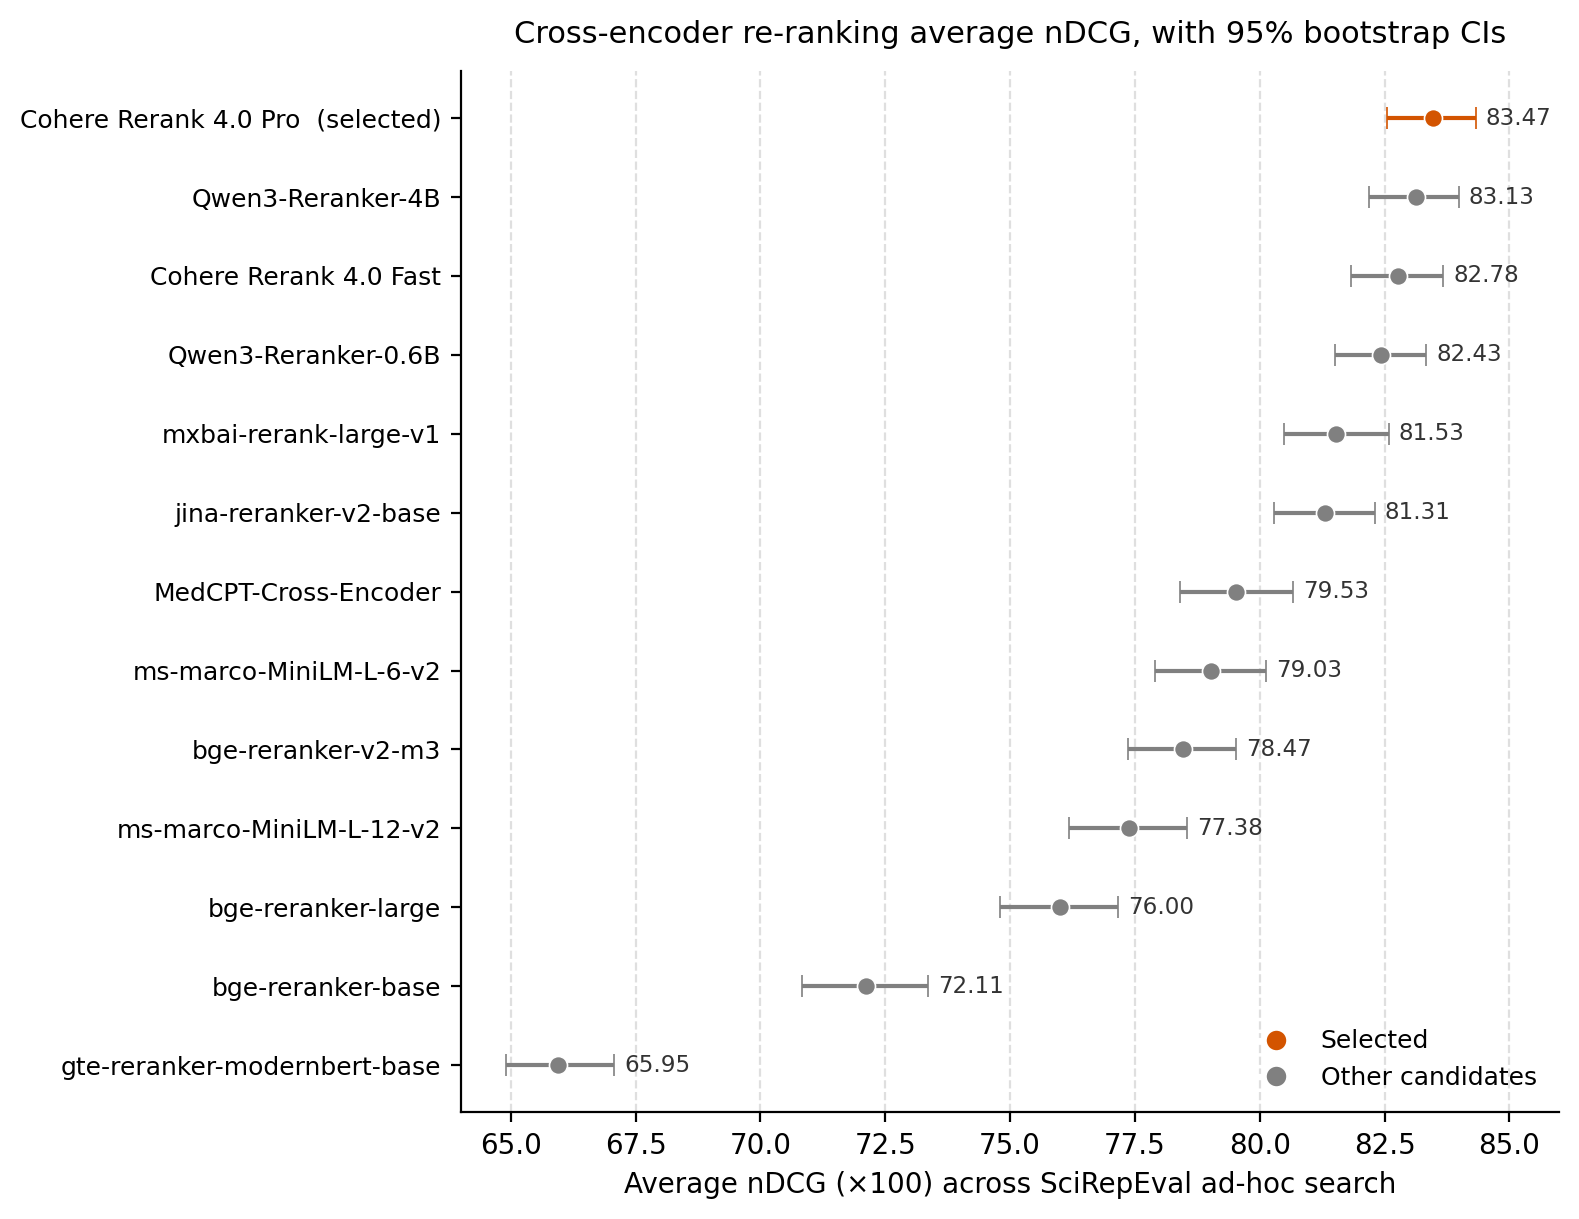
\includegraphics[width=\columnwidth]{images/data_and_results/crossencoder_average.png}
\caption{Cross-encoder re-ranking average nDCG across the three SciRepEval ad-hoc search tasks, with 95 percent bootstrap confidence intervals from 1000 resamples. The selected model is shown in orange.}
\label{fig:xenc-avg}
\end{figure}

\begin{figure}[t]
\centering
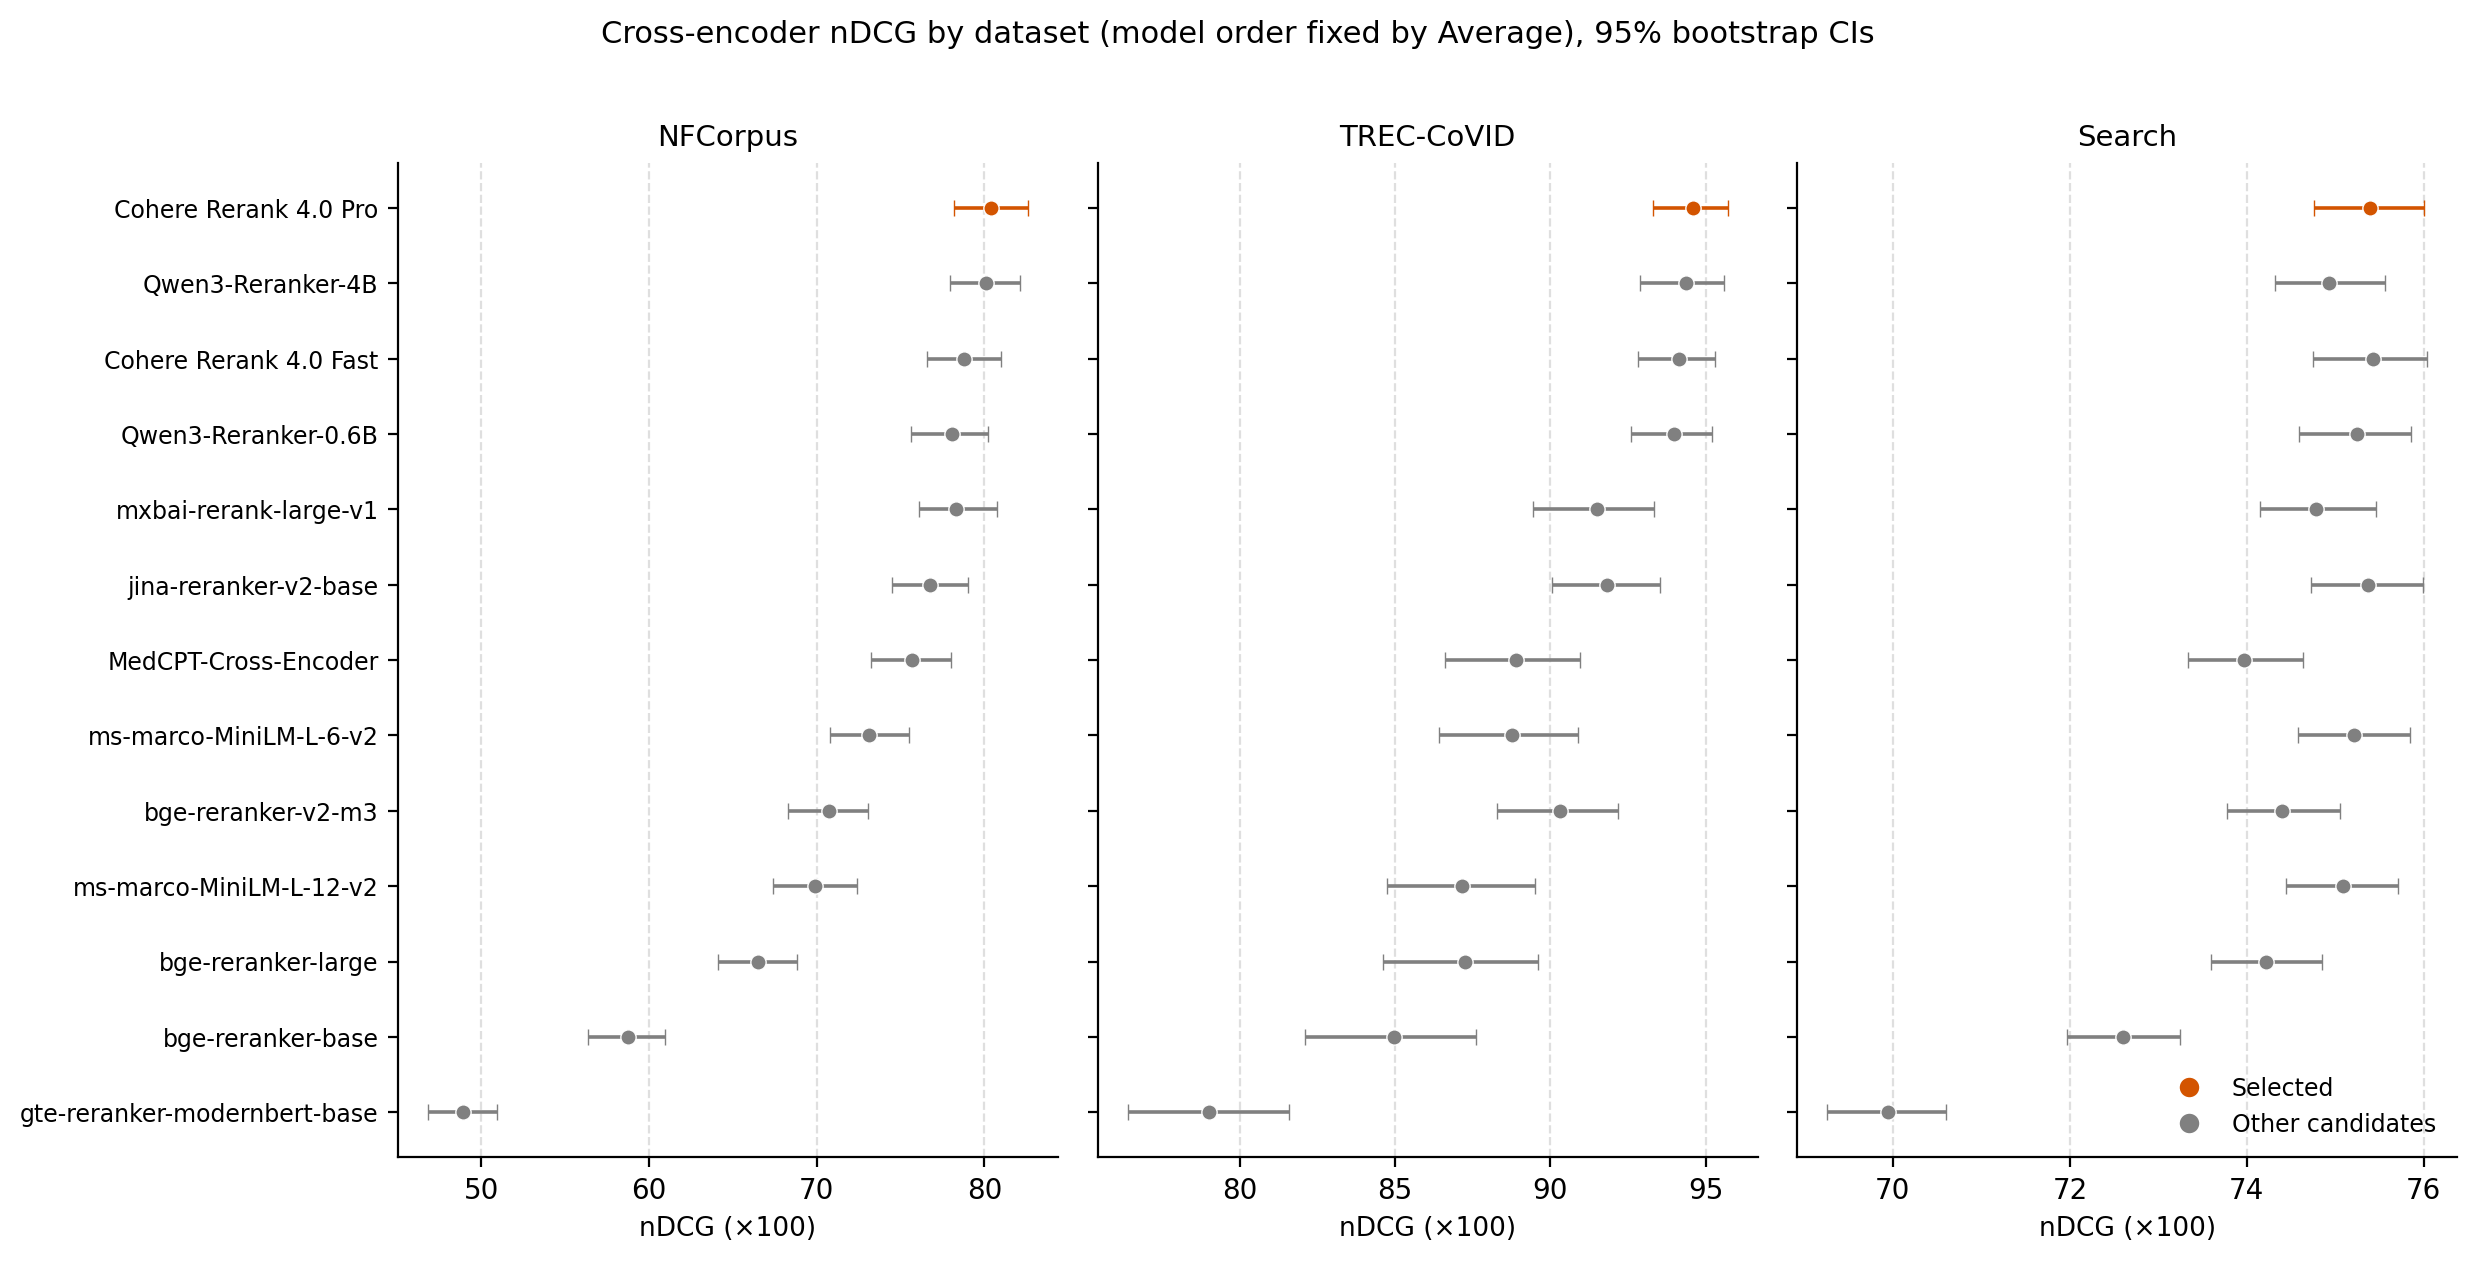
\includegraphics[width=\columnwidth]{images/data_and_results/crossencoder_by_dataset.png}
\caption{Cross-encoder nDCG on each SciRepEval ad-hoc search task, with models held in their Average order for comparison and 95 percent bootstrap confidence intervals. The selected model is shown in orange.}
\label{fig:xenc-pertask}
\end{figure}

Cohere Rerank 4.0 Pro was selected as the cross-encoder. The candidate rerankers were evaluated on the same three SciRepEval ad-hoc search tasks as the bi-encoder and under the same nDCG metric, scoring each model by the ranking it produces when it re-ranks the retrieved candidate pool. All scores are nDCG $\times$100 with 95 percent bootstrap intervals from 1000 resamples. The intervals are tight on Search, which has 2585 queries, and wide on TREC-CoVID, which has 50.

Table~\ref{tab:xenc-results} reports the full per-task and average scores, and Figure~\ref{fig:xenc-avg} plots each model's average with its interval. The selected model holds the highest average at 83.47. Its interval overlaps those of the next three models, Qwen3-Reranker-4B at 83.13, Cohere Rerank 4.0 Fast at 82.78, and Qwen3-Reranker-0.6B at 82.43, so these four form a statistical tie at the top. Within that group the strongest self-hostable model, Qwen3-Reranker-4B, is tied with the selected model. Below the leading four the field descends steadily through a long tail to gte-reranker-modernbert-base at 65.95, a spread of more than seventeen points from top to bottom.

The per-task view in Figure~\ref{fig:xenc-pertask} shows that almost all of this separation comes from NFCorpus, where the models spread across more than thirty points, from 80.42 at the top down to 48.88. Search behaves in the opposite way. Every reranker scores close to 75, since the small candidate pool the stage re-ranks leaves little room to reorder, so the task barely separates the models. TREC-CoVID falls between the two, with a high but noisy spread that reflects its fifty queries.

\begin{table*}[t]
\caption{Deployment characteristics of the candidate cross-encoders.}
\label{tab:xenc-deploy}
\centering
\footnotesize
\begin{tabular}{@{}p{4.5cm}llp{4.0cm}@{}}
\toprule
Model & Params (approx.) & Precision & Self-hostable \\
\midrule
Cohere Rerank 4.0 Pro & undisclosed & n/a & no (paid API) \\
Qwen3-Reranker-4B & $\sim$4 B & int8 & yes (Apache-2.0) \\
Cohere Rerank 4.0 Fast & undisclosed & n/a & no (paid API) \\
Qwen3-Reranker-0.6B & $\sim$0.6 B & fp16 & yes (Apache-2.0) \\
mxbai-rerank-large-v1 & $\sim$435 M & fp16 & yes \\
jina-reranker-v2-base & $\sim$278 M & fp16 & weights CC-BY-NC (non-commercial) \\
MedCPT-Cross-Encoder & $\sim$109 M & fp16 & yes \\
ms-marco-MiniLM-L-6-v2 & $\sim$22 M & fp16 & yes \\
bge-reranker-v2-m3 & $\sim$568 M & fp16 & yes \\
ms-marco-MiniLM-L-12-v2 & $\sim$33 M & fp16 & yes \\
bge-reranker-large & $\sim$560 M & fp16 & yes \\
bge-reranker-base & $\sim$278 M & fp16 & yes \\
gte-reranker-modernbert-base & $\sim$150 M & fp16 & yes \\
\bottomrule
\end{tabular}

\vspace{3pt}
\begin{minipage}{\linewidth}
\footnotesize\itshape
Unlike the bi-encoder, a reranker stores no vectors, so its cost is latency, which scales with parameter count, rather than memory, which is why the stage runs over only around 100 candidates. The Qwen3 rerankers are released under Apache-2.0, while the jina-reranker-v2 weights are CC-BY-NC-4.0 and so are non-commercial and not deployable in a commercial product. The remaining licences should be confirmed against the deployment terms before selection.
\end{minipage}
\end{table*}

Table~\ref{tab:xenc-deploy} records the deployment characteristics, namely approximate parameter count, precision, and whether the model is self-hostable along with its licence. Unlike the bi-encoder, a reranker stores no vectors, so its cost is latency rather than memory and scales with parameter count, which is the reason the stage runs over only around 100 candidates. The self-hostable options carry mixed licences, with the Qwen3 rerankers released under Apache-2.0 and the jina reranker under a non-commercial CC-BY-NC licence, while the selected model is served through a paid API.

% ----------------------------------------------------------------------------
\subsection{Embedding Quantisation}
% Placeholder. Results not yet available.
\textit{[Placeholder. Results comparing int8 against full-precision nDCG, and the resulting accuracy cost, to be added.]}

% ----------------------------------------------------------------------------
\subsection{System-Level Evaluation}
% Placeholder. Results not yet available.
\textit{[Placeholder. End-to-end results over a realistic query set with light relevance judgments to be added.]}   (or \include{...})
%
%  Requires in the preamble of main.tex:
%      \usepackage{booktabs}
%      \usepackage{graphicx}
%      \usepackage{array}      % only if you later add >{...} column types
%
%  Figures use placeholder paths under figures/ -- replace with your exports.
%  Tables and figures are referenced with \ref so numbering stays dynamic and
%  any table can be moved to an appendix without breaking the prose.
% ============================================================================

\section{Data and Results}

This section reports the result of each component benchmark from the validation design in Section~II-D, taking the components in turn.

% ----------------------------------------------------------------------------
\subsection{Keyword Generation}

\begin{table}[t]
\caption{KPBiomed keyword extraction, present and absent F1@5 with stemming. Models are ordered by present F1, and GPT-5.4-nano is the deployed model.}
\label{tab:kw-kpbiomed}
\centering
\footnotesize
\begin{tabular}{@{}lrr@{}}
\toprule
Model & Present F1@5 & Absent F1@5 \\
\midrule
\textbf{GPT-5.4-nano} & \textbf{30.86} & 1.95 \\
MultipartiteRank & 19.58 & 0.00 \\
TF-IDF & 18.56 & 0.04 \\
KeyBART & 17.40 & \textbf{2.07} \\
YAKE & 16.79 & 0.02 \\
KBIR-inspec & 16.36 & 0.01 \\
KeyBERT-MiniLM & 8.52 & 0.04 \\
TextRank & 5.11 & 0.00 \\
\bottomrule
\end{tabular}
\end{table}

\begin{figure*}[t]
\centering
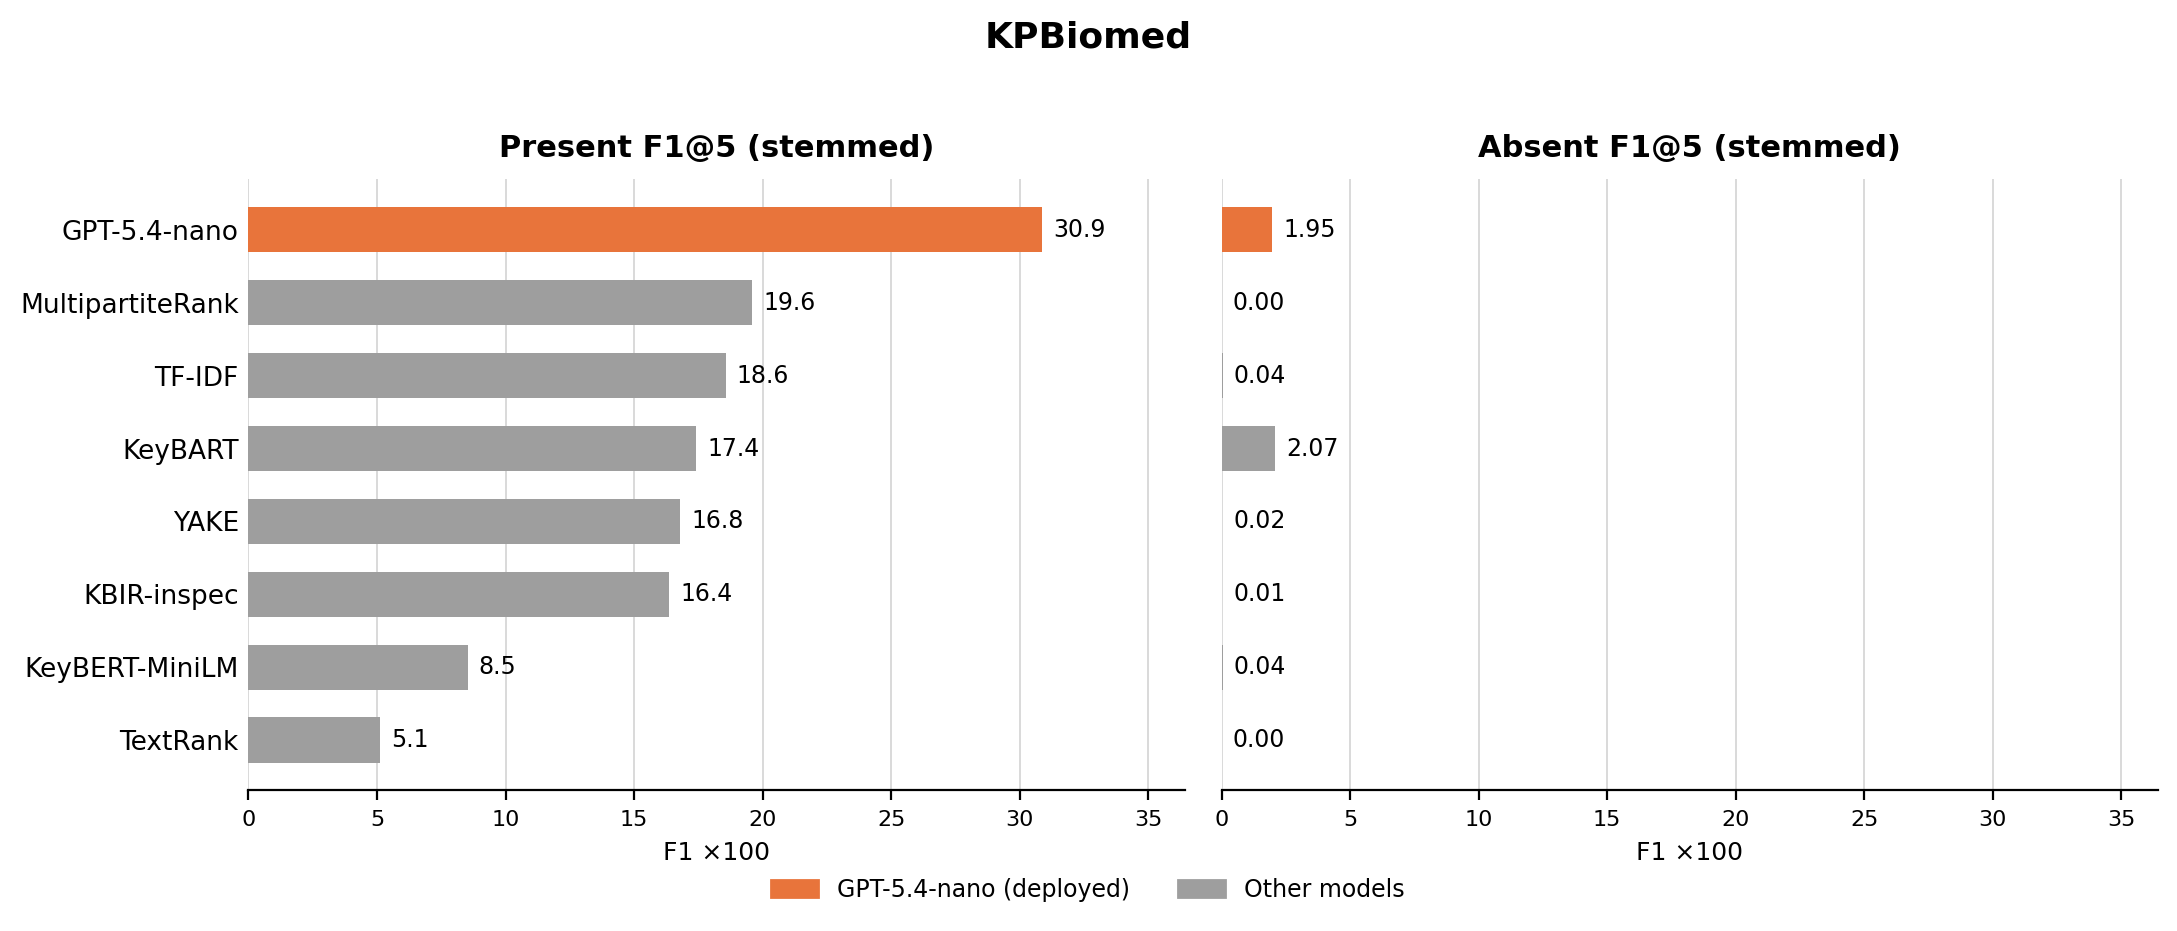
\includegraphics[width=\textwidth]{images/data_and_results/keyword_kpbiomed.png}
\caption{KPBiomed keyword extraction, present and absent F1@5 by model with stemming. The deployed model GPT-5.4-nano is shown in orange and the remaining baselines in grey.}
\label{fig:kw-kpbiomed}
\end{figure*}

\begin{table}[t]
\caption{OAGKX keyword extraction, present and absent F1@5 with stemming. Models are ordered by present F1, and GPT-5.4-nano is the deployed model.}
\label{tab:kw-oagkx}
\centering
\footnotesize
\begin{tabular}{@{}lrr@{}}
\toprule
Model & Present F1@5 & Absent F1@5 \\
\midrule
KeyBART & \textbf{28.42} & \textbf{5.09} \\
\textbf{GPT-5.4-nano} & 26.49 & 1.77 \\
KBIR-inspec & 20.16 & 0.05 \\
MultipartiteRank & 18.83 & 0.00 \\
TF-IDF & 15.55 & 0.03 \\
KeyBERT-MiniLM & 12.04 & 0.04 \\
TextRank & 11.15 & 0.02 \\
YAKE & 8.85 & 0.00 \\
\bottomrule
\end{tabular}
\end{table}

\begin{figure*}[t]
\centering
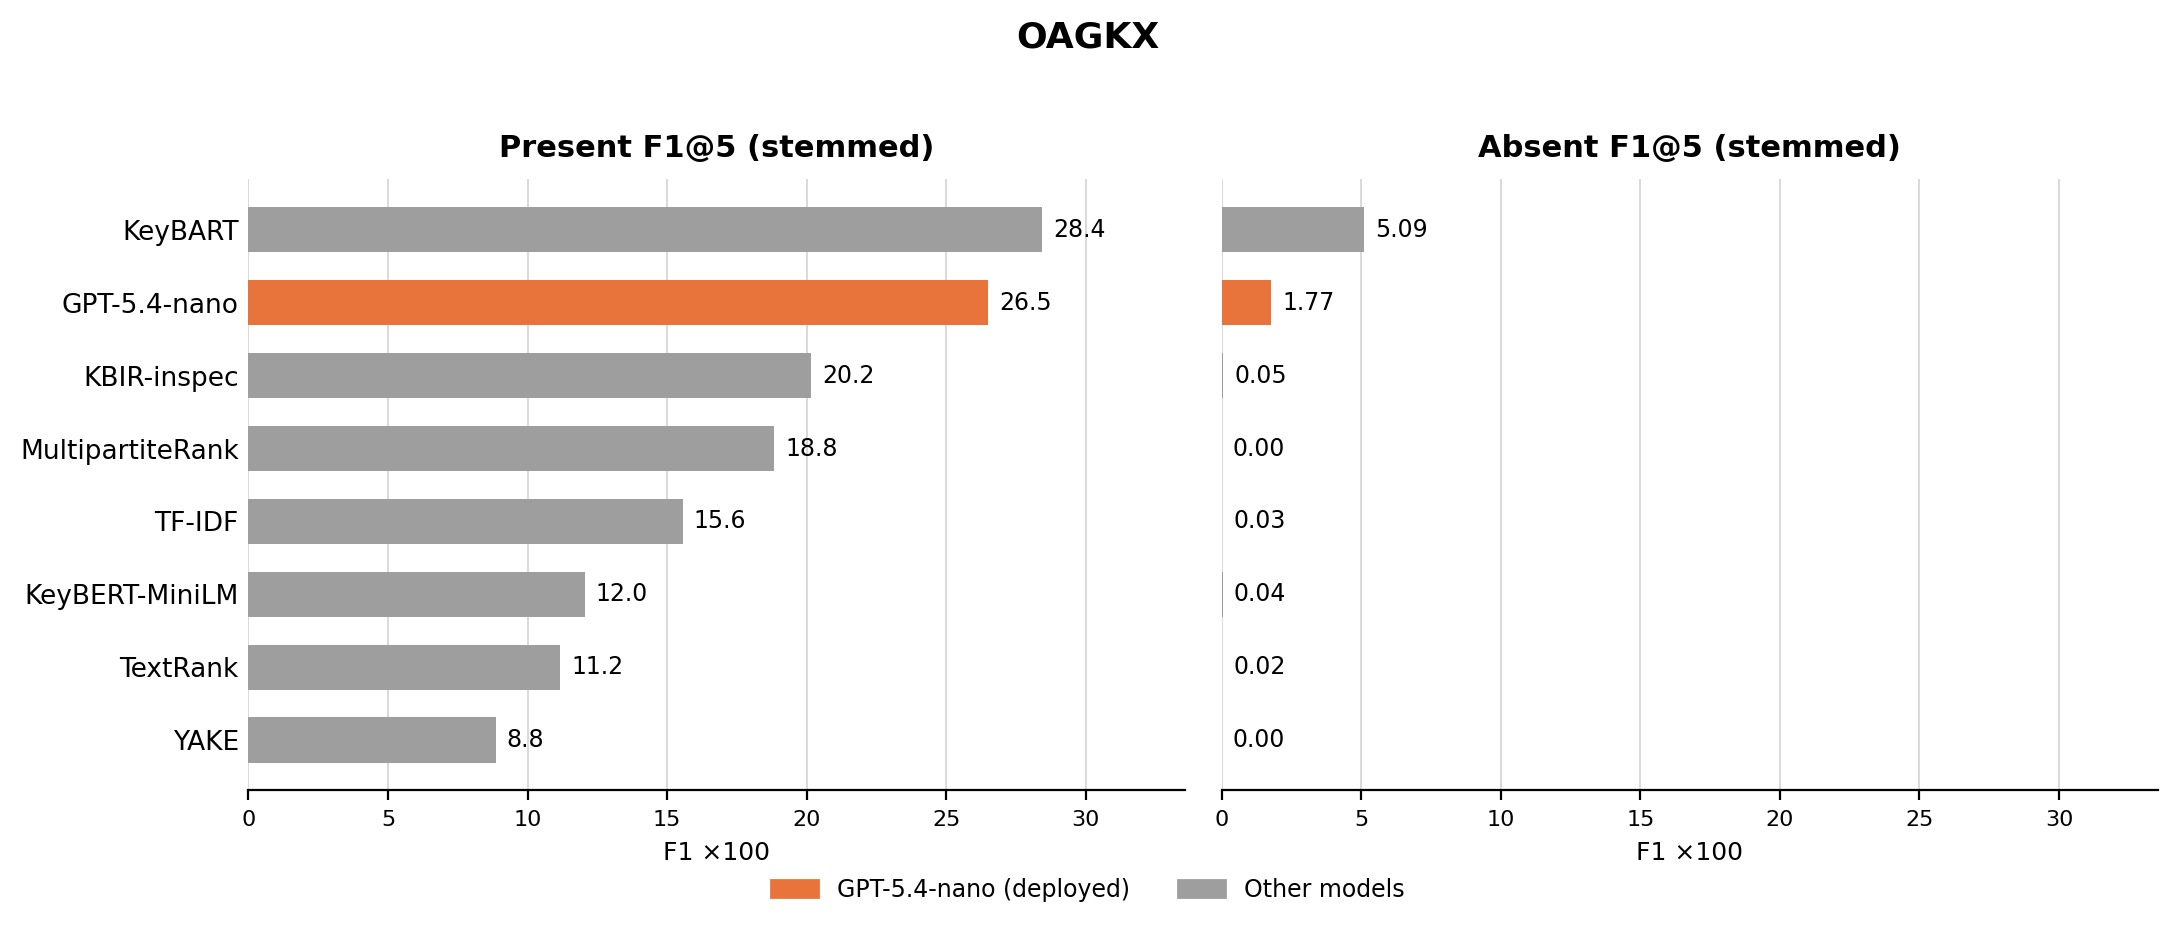
\includegraphics[width=\textwidth]{images/data_and_results/keyword_oagkx.png}
\caption{OAGKX keyword extraction, present and absent F1@5 by model with stemming. The deployed model GPT-5.4-nano is shown in orange and the remaining baselines in grey.}
\label{fig:kw-oagkx}
\end{figure*}

\begin{table}[t]
\caption{PubMedAKE keyword extraction, present and absent F1@5 with stemming. Models are ordered by present F1, and GPT-5.4-nano is the deployed model.}
\label{tab:kw-pubmedake}
\centering
\footnotesize
\begin{tabular}{@{}lrr@{}}
\toprule
Model & Present F1@5 & Absent F1@5 \\
\midrule
\textbf{GPT-5.4-nano} & \textbf{36.44} & \textbf{1.30} \\
TF-IDF & 24.06 & 0.03 \\
MultipartiteRank & 23.06 & 0.00 \\
KBIR-inspec & 19.36 & 0.01 \\
KeyBART & 18.41 & 1.29 \\
YAKE & 12.92 & 0.01 \\
KeyBERT-MiniLM & 6.78 & 0.01 \\
TextRank & 4.68 & 0.00 \\
\bottomrule
\end{tabular}
\end{table}

\begin{figure*}[t]
\centering
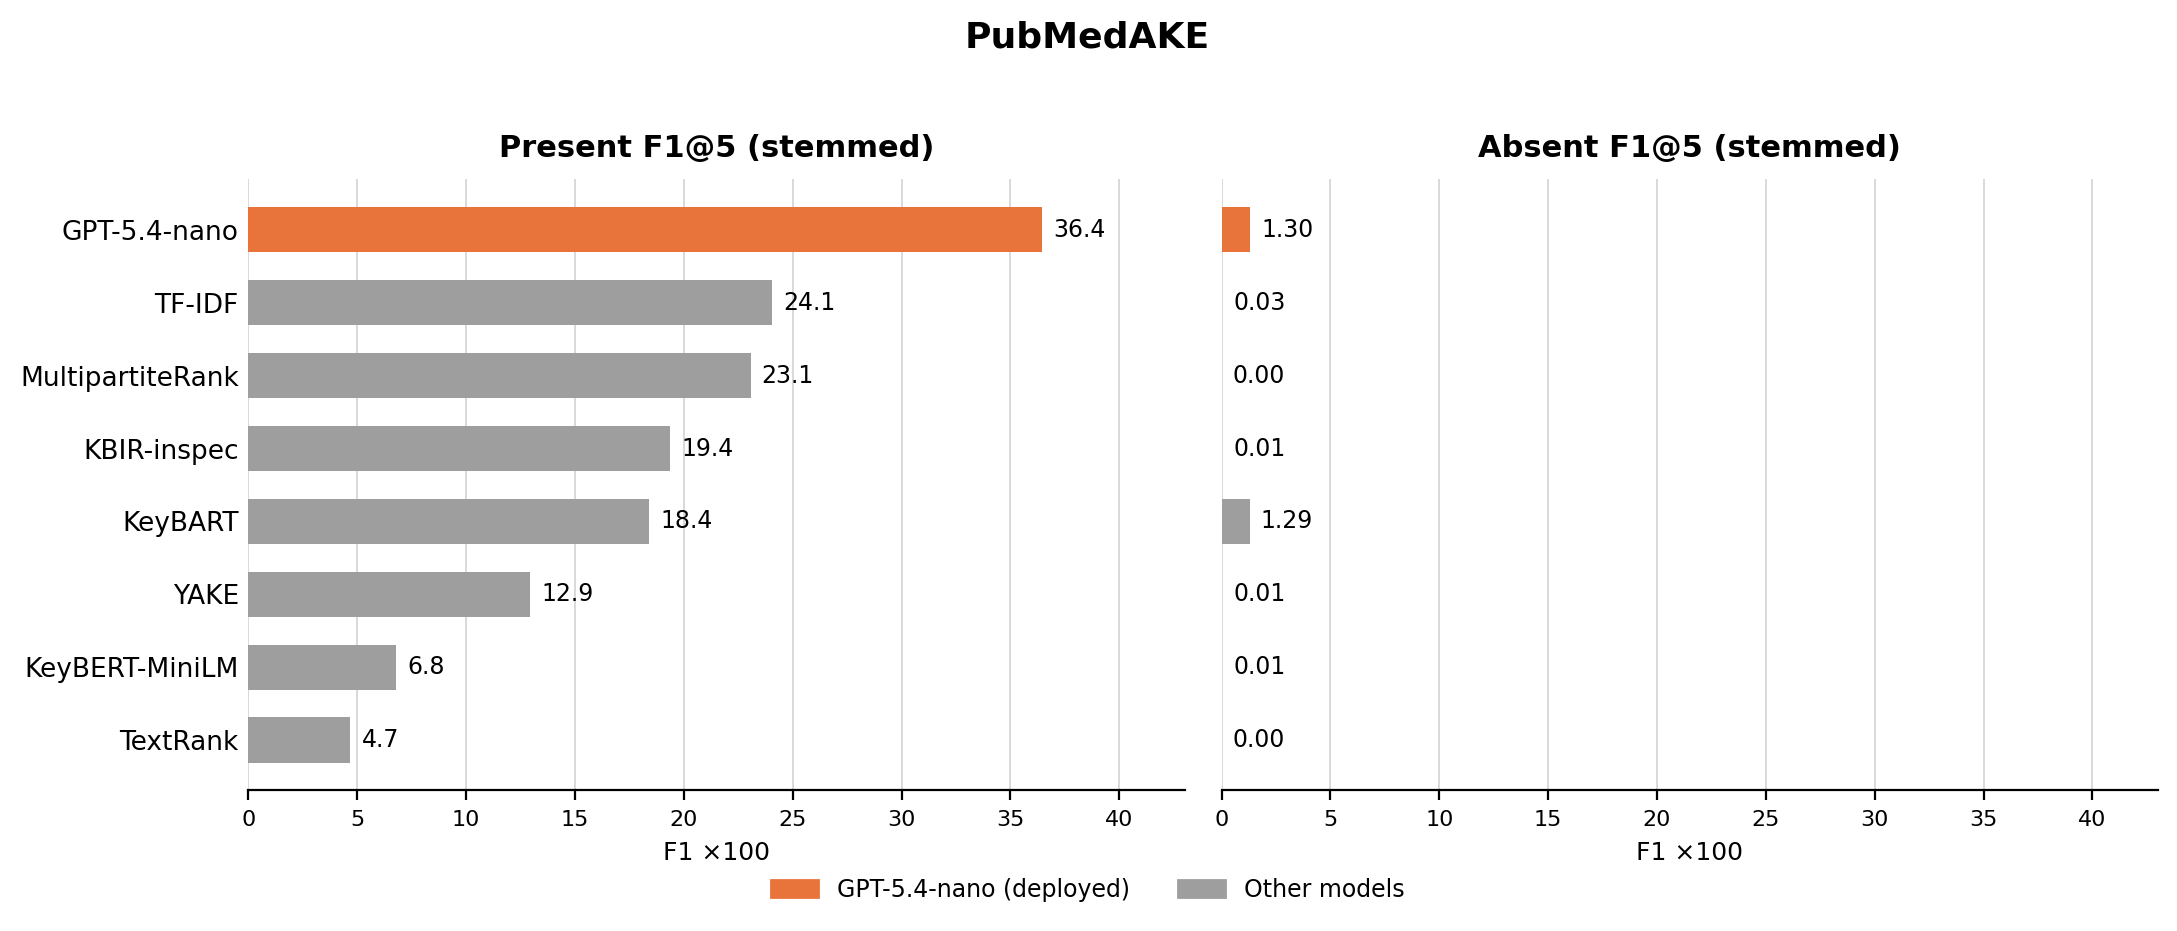
\includegraphics[width=\textwidth]{images/data_and_results/keyword_pubmedake.png}
\caption{PubMedAKE keyword extraction, present and absent F1@5 by model with stemming. The deployed model GPT-5.4-nano is shown in orange and the remaining baselines in grey.}
\label{fig:kw-pubmedake}
\end{figure*}

GPT-5.4-nano was benchmarked for keyword generation against a set of statistical and neural baselines on KPBiomed, OAGKX, and PubMedAKE. Tables~\ref{tab:kw-kpbiomed} to~\ref{tab:kw-pubmedake} report the results for each dataset in turn. Throughout, present (extractive) keyphrases, which occur verbatim in the source text, are distinguished from absent (abstractive) keyphrases, which do not and so must be generated. Matches are scored by F1 at five with light stemming, so that a keyphrase and its stem count as a match while a different word of the same meaning does not.

On the present keyphrase tasks, GPT-5.4-nano records the highest score on KPBiomed and PubMedAKE and the second highest on OAGKX, where KeyBART leads. Its margin is widest on PubMedAKE, at 36.44 against a next-best of 24.06.

On the absent keyphrase tasks, which a model can only score on by producing keyphrases that do not occur in the source text, GPT-5.4-nano scores in the low single digits, from 1.30 on PubMedAKE to 1.95 on KPBiomed. These non-zero scores indicate that the model generates a small portion of its keyphrases rather than extracting all of them. The other generative baseline, KeyBART, behaves similarly and records the highest absent score on KPBiomed and OAGKX. The statistical extractors such as TF-IDF, YAKE, TextRank, and MultipartiteRank remain near zero here, since they return only spans found in the source text and so do not generate at all.

\begin{table}[t]
\caption{Keyword extraction stability for GPT-5.4-nano over three runs on a 2000-document sample.}
\label{tab:kw-stability}
\centering
\footnotesize
\begin{tabular}{@{}p{0.66\columnwidth}r@{}}
\toprule
Quantity & Value \\
\midrule
Set-level Jaccard across runs & 0.73 \\
Present-F1 run-to-run std & $\pm$0.07 \\
Deterministic baselines (TF-IDF, YAKE, TextRank, MultipartiteRank, KeyBERT, KBIR) & 1.00 \\
\bottomrule
\end{tabular}
\end{table}

Table~\ref{tab:kw-stability} reports a reproducibility check for GPT-5.4-nano over three runs on a 2000-document sample. The set-level Jaccard similarity across runs is 0.73, meaning that for a given document around 73 percent of the combined set of keyphrases from any two runs is shared by both, equivalent to roughly one in six keyphrases changing between runs. The model is therefore largely repeatable but not deterministic, unlike the baselines, which are reproducible by construction. The effect on measured performance is negligible, with a run-to-run present-F1 standard deviation of 0.07. The same sample also reproduces the full-split figures to within roughly a tenth of a point, confirming that the smaller stability sample does not shift the headline results.

% ----------------------------------------------------------------------------
\subsection{IR Extraction}

\begin{table*}[t]
\caption{Natural-language-to-IR accuracy by model. Joint IR accuracy counts a query as correct when both its entities and its boolean expression are correct under exact matching, reported in the as-deployed or best configuration for each model.}
\label{tab:ir-accuracy}
\centering
\footnotesize
\begin{tabular}{@{}lllcc@{}}
\toprule
Model & Host & Configuration & IR accuracy & 95\% CI \\
\midrule
\textbf{gpt-5.4-nano} & Azure & default, 0 reasoning tok & \textbf{0.937}$^{\dagger}$ & [0.897, 0.983] \\
gpt-5-mini & Azure & default, 384 reasoning tok & 0.931 & [0.879, 0.974] \\
qwen3:8b & Local (Q4) & single-shot & 0.802 & [0.733, 0.871] \\
qwen3:4b & Local (Q4) & thinking$^{\ddagger}$ & 0.784 & [0.707, 0.862] \\
qwen2.5:3b & Local (Q4) & non-reasoning & 0.207 & [0.138, 0.284] \\
phi4-mini & Local (Q4) & non-reasoning & 0.052 & [0.017, 0.095] \\
llama3.2:3b & Local (Q4) & non-reasoning & 0.026 & [0.000, 0.060] \\
\bottomrule
\end{tabular}

\vspace{3pt}
\begin{minipage}{\linewidth}
\footnotesize\itshape
Confidence intervals are 95 percent bootstrap over 1000 iterations. Cross-model gaps that fall within these intervals are treated as ties, and bold marks the deployed model. The dagger denotes a three-run mean, whose single-run range is 0.914 to 0.940, with temperature zero returning a byte-identical output on 96.6 percent of queries (Table~\ref{tab:ir-stability}). The double dagger denotes qwen3:4b, whose single-shot configuration produced degenerate empty output, so its thinking configuration is its only usable score.
\end{minipage}
\end{table*}

\begin{figure}[t]
\centering
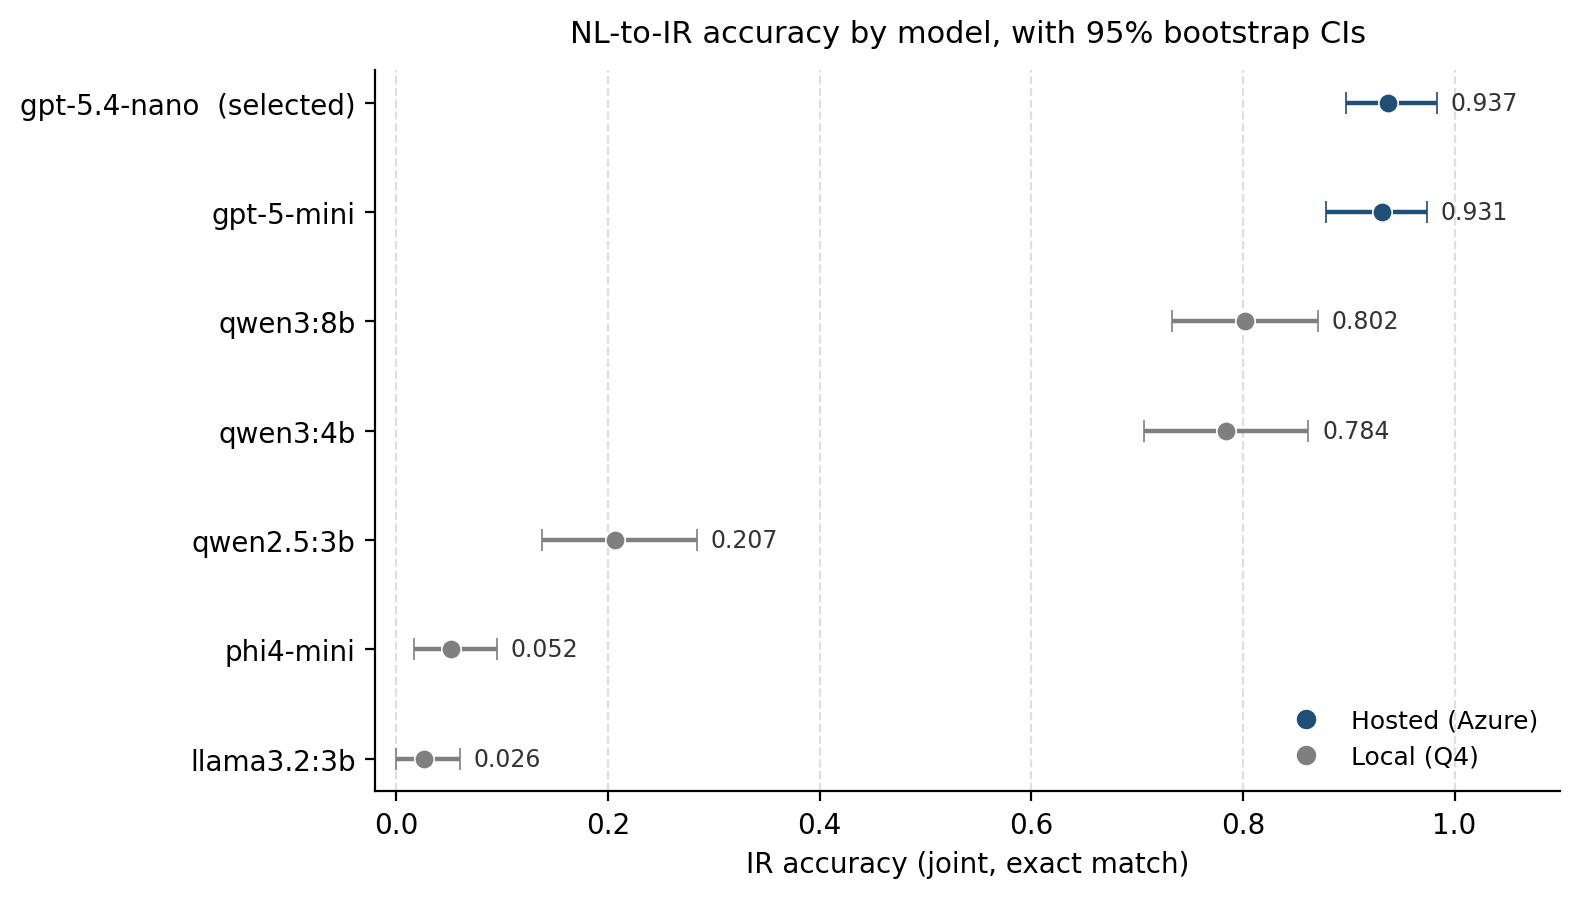
\includegraphics[width=\columnwidth]{images/data_and_results/ir_accuracy_ci.png}
\caption{Natural-language-to-IR joint accuracy by model on the hand-built gold set, with 95 percent bootstrap confidence intervals from 1000 resamples.}
\label{fig:ir-accuracy}
\end{figure}

GPT-5.4-nano was benchmarked for natural-language-to-IR extraction against a set of hosted and local models on a hand-built gold set of queries paired with their correct intermediate representations. The set was constructed to exercise every entity type the system supports across a range of boolean structures, from single topics through to bracketed combinations of AND, OR, and NOT, so that performance on it reflects the input and output behaviour the system actually requires. The headline measure, IR accuracy, is the joint figure reported in Table~\ref{tab:ir-accuracy}, counting a query as correct only when both its extracted entities and its boolean expression are correct under exact matching.

Figure~\ref{fig:ir-accuracy} plots each model's accuracy with its 95 percent bootstrap interval. The two hosted models lead the benchmark by a clear margin, with GPT-5.4-nano highest at an IR accuracy of 0.937 and GPT-5-mini close behind at 0.931. Both hosted intervals clear those of every local model without overlap, placing the hosted advantage beyond sampling noise, while the two overlap each other and are statistically indistinguishable. Among the local models, the two strongest (qwen3:8b and qwen3:4b) reach around 0.80, and the three smaller models fall away sharply to 0.207, 0.052, and 0.026, near the floor of the task.

\begin{table}[t]
\caption{Effect of reasoning on IR accuracy.}
\label{tab:ir-reasoning}
\centering
\footnotesize
\begin{tabular}{@{}lccc@{}}
\toprule
Model & Reasoning off & Reasoning on & $\Delta$ \\
\midrule
gpt-5.4-nano & 0.914 & 0.922 & +0.008 \\
gpt-5-mini & \textbf{0.750} & \textbf{0.940} & \textbf{+0.190} \\
\bottomrule
\end{tabular}

\vspace{3pt}
\begin{minipage}{\linewidth}
\footnotesize\itshape
Reasoning is controlled through the Azure \texttt{reasoning\_effort} setting with tokens accounted. Reasoning on used approximately 246 tokens per query for gpt-5.4-nano and 896 for gpt-5-mini, while reasoning off used none. Reasoning lifts the weaker model in each tier, while the stronger one is already at its ceiling.
\end{minipage}
\end{table}

Table~\ref{tab:ir-reasoning} isolates the effect of reasoning on the two GPT models. GPT-5.4-nano gains almost nothing from it, moving from 0.914 without reasoning to 0.922 with around 246 reasoning tokens, a difference of 0.008, and so reaches its accuracy in a single pass with no reasoning budget. GPT-5-mini behaves differently, scoring only 0.750 without reasoning and rising to 0.940 once reasoning is enabled, at a cost of around 896 reasoning tokens per query. The stronger model is already at its ceiling unaided, whereas the weaker one becomes competitive only by spending a substantial token budget.

\begin{table}[t]
\caption{Deployed model, metric decomposition in the default-effort configuration.}
\label{tab:ir-decomp}
\centering
\footnotesize
\begin{tabular}{@{}lcc@{}}
\toprule
Metric & Value & 95\% CI \\
\midrule
IR accuracy (joint) & 0.937 & [0.897, 0.983] \\
Entity F1 (micro) & 0.984 & [0.969, 0.995] \\
Entity F1 (macro) & 0.982 & [0.967, 0.994] \\
Expression equivalence & 0.931 & [0.888, 0.974] \\
Expression graded & 0.985 & [0.974, 0.995] \\
\bottomrule
\end{tabular}

\vspace{3pt}
\begin{minipage}{\linewidth}
\footnotesize\itshape
Joint accuracy is bounded by expression equivalence, since entity extraction almost never fails on its own.
\end{minipage}
\end{table}

\begin{table}[t]
\caption{Deployed model, accuracy by stratum, ordered hardest first.}
\label{tab:ir-stratum}
\centering
\footnotesize
\begin{tabular}{@{}lrrr@{}}
\toprule
Stratum & $n$ & IR accuracy & failures \\
\midrule
\texttt{filter\_distractor} & 10 & 0.700 & 3 \\
\texttt{multi\_negation} & 10 & 0.800 & 2 \\
\texttt{deep\_nested} & 12 & 0.833 & 2 \\
\texttt{hard\_typing} & 12 & 0.917 & 1 \\
\texttt{single\_concept} & 6 & 1.000 & 0 \\
\texttt{multi\_concept} & 12 & 1.000 & 0 \\
\texttt{exclusion} & 12 & 1.000 & 0 \\
\texttt{nested} & 12 & 1.000 & 0 \\
\texttt{mixed\_entity} & 16 & 1.000 & 0 \\
\texttt{review\_style} & 14 & 1.000 & 0 \\
\bottomrule
\end{tabular}

\vspace{3pt}
\begin{minipage}{\linewidth}
\footnotesize\itshape
The count $n$ is small per stratum, at sixteen or fewer, so the failure counts are a more reliable read than the rate, and the per-stratum 95 percent intervals are wide, for example \texttt{filter\_distractor} at 0.700 is seven of ten.
\end{minipage}
\end{table}

Tables~\ref{tab:ir-decomp} and~\ref{tab:ir-stratum} decompose the chosen model's performance, which is strong across both components and most query types. By component, entity extraction is near-perfect, with a micro F1 of 0.984 and a macro F1 of 0.982, while expression equivalence is lower at 0.931 (a graded variant that credits partially correct expressions reaches 0.985). The joint IR accuracy of 0.937 is therefore bounded by the expression score, since entity extraction almost never fails on its own. By query type, the model is perfect on six of the ten strata, covering single and multiple concepts, exclusions, nesting, mixed entities, and review-style queries. Its errors concentrate in the remaining four. The largest source is \texttt{filter\_distractor}, where three of ten queries fail because the model miscategorises a filter term such as a year or citation bound as a searchable entity. The rest fall on the structurally hardest queries, with two of ten failing on multiple negations, two of twelve on deep nesting, and one of twelve on hard typing. Per-stratum counts are small, at sixteen queries or fewer, so the failure counts are a more reliable read than the rates.

\begin{table}[t]
\caption{Stability of the deployed model over three runs.}
\label{tab:ir-stability}
\centering
\footnotesize
\begin{tabular}{@{}p{0.46\columnwidth}cc@{}}
\toprule
Metric & temp 0 & temp 0.7 \\
\midrule
IR identical across all 3 runs & 0.966 & 0.957 \\
Run-to-run IR-accuracy std & 0.004 & 0.004 \\
Majority-vote@3 vs single run & 0.931 vs 0.940 & 0.940 vs 0.940 \\
\bottomrule
\end{tabular}

\vspace{3pt}
\begin{minipage}{\linewidth}
\footnotesize\itshape
Temperature zero is highly but not perfectly deterministic, and majority voting adds nothing.
\end{minipage}
\end{table}

Table~\ref{tab:ir-stability} reports a stability check over three runs. Although GPT-5.4-nano is not deterministic, at temperature zero it returns an identical IR on 96.6 percent of queries, with a run-to-run accuracy standard deviation of 0.004. Aggregating three runs by majority vote changes nothing, at 0.931 against 0.940 for a single run, so the three-run mean of 0.937 reported in Table~\ref{tab:ir-accuracy} is used throughout.

% ----------------------------------------------------------------------------
\subsection{Dense Bi-encoder Retrieval}

\begin{table*}[t]
\caption{Dense bi-encoder retrieval on SciRepEval ad-hoc search, nDCG $\times$100 with 95 percent bootstrap confidence intervals.}
\label{tab:bienc-results}
\centering
\scriptsize
\setlength{\tabcolsep}{4pt}
\begin{tabular}{@{}p{3.0cm}llll@{}}
\toprule
Model & NFCorpus & TREC-CoVID & Search & Average \\
\midrule
Qwen3-Embedding-4B (int8) & \textbf{80.02 [77.75, 82.17]} & \textbf{94.28 [92.96, 95.43]} & 75.54 [74.93, 76.17] & \textbf{83.28 [82.35, 84.19]} \\
EmbeddingGemma-300M & 79.13 [76.84, 81.29] & 92.45 [90.68, 94.03] & 75.32 [74.66, 75.93] & 82.30 [81.32, 83.31] \\
Qwen3-Embedding-0.6B & 77.94 [75.75, 80.22] & 93.90 [92.52, 95.10] & 75.03 [74.41, 75.65] & 82.29 [81.32, 83.25] \\
text-embedding-3-small (existing) & 78.78 [76.61, 81.05] & 92.38 [90.58, 93.96] & 75.14 [74.52, 75.74] & 82.10 [81.08, 83.05] \\
mxbai-embed-large-v1 & 79.37 [77.19, 81.72] & 91.77 [90.02, 93.25] & 74.92 [74.29, 75.56] & 82.02 [81.06, 82.96] \\
SPECTER2-adhoc-query & 70.46 [68.01, 72.97] & 90.08 [87.84, 92.13] & \textbf{78.22 [77.60, 78.86]} & 79.59 [78.46, 80.71] \\
BGE-M3 & 74.05 [71.72, 76.35] & 89.21 [87.08, 91.16] & 74.82 [74.20, 75.46] & 79.36 [78.29, 80.42] \\
SPECTER2-base (existing) & 72.03 [69.60, 74.54] & 89.46 [86.99, 91.58] & 73.76 [73.12, 74.41] & 78.42 [77.27, 79.58] \\
\bottomrule
\end{tabular}

\vspace{3pt}
\begin{minipage}{\linewidth}
\footnotesize\itshape
The metric is SciRepEval ad-hoc-search full-ranking nDCG over a per-query candidate pool, not BEIR full-corpus nDCG@10. Confidence intervals are 95 percent bootstrap [lo, hi] over 1000 iterations with seed 42, and bold marks the best point estimate per column. On Average the top five models' intervals overlap, a statistical tie, and SPECTER2-adhoc-query's Search lead is the one between-model gap whose interval clears the general models.
\end{minipage}
\end{table*}

\begin{figure}[t]
\centering
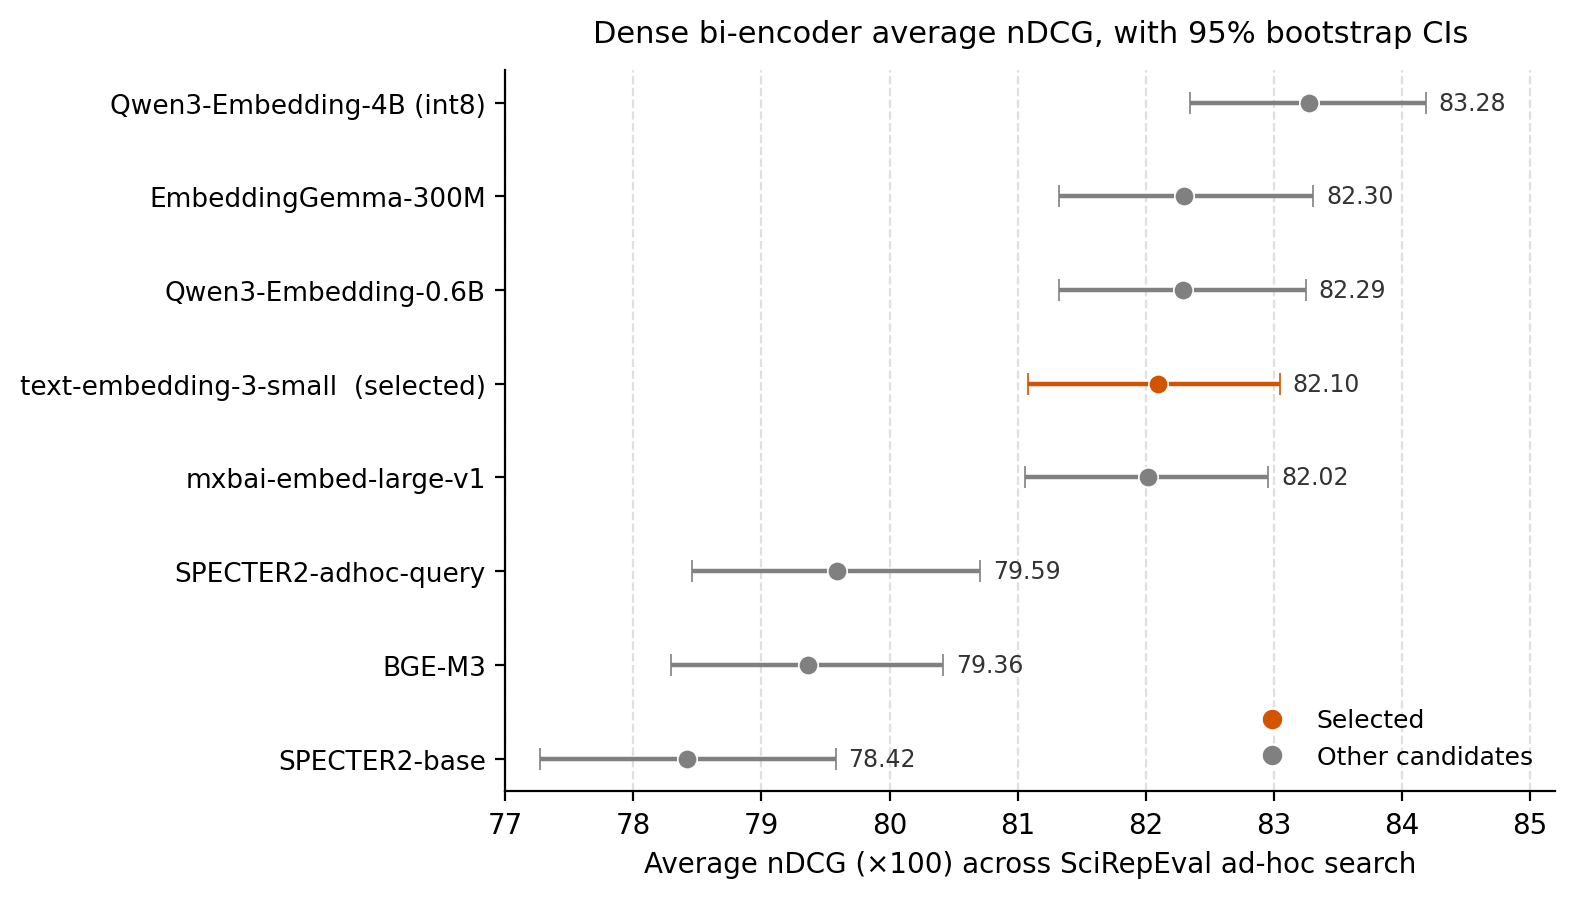
\includegraphics[width=\columnwidth]{images/data_and_results/biencoder_average.png}
\caption{Dense bi-encoder average nDCG across the three SciRepEval ad-hoc search tasks, with 95 percent bootstrap confidence intervals from 1000 resamples. The selected model is shown in orange.}
\label{fig:bienc-avg}
\end{figure}

\begin{figure}[t]
\centering
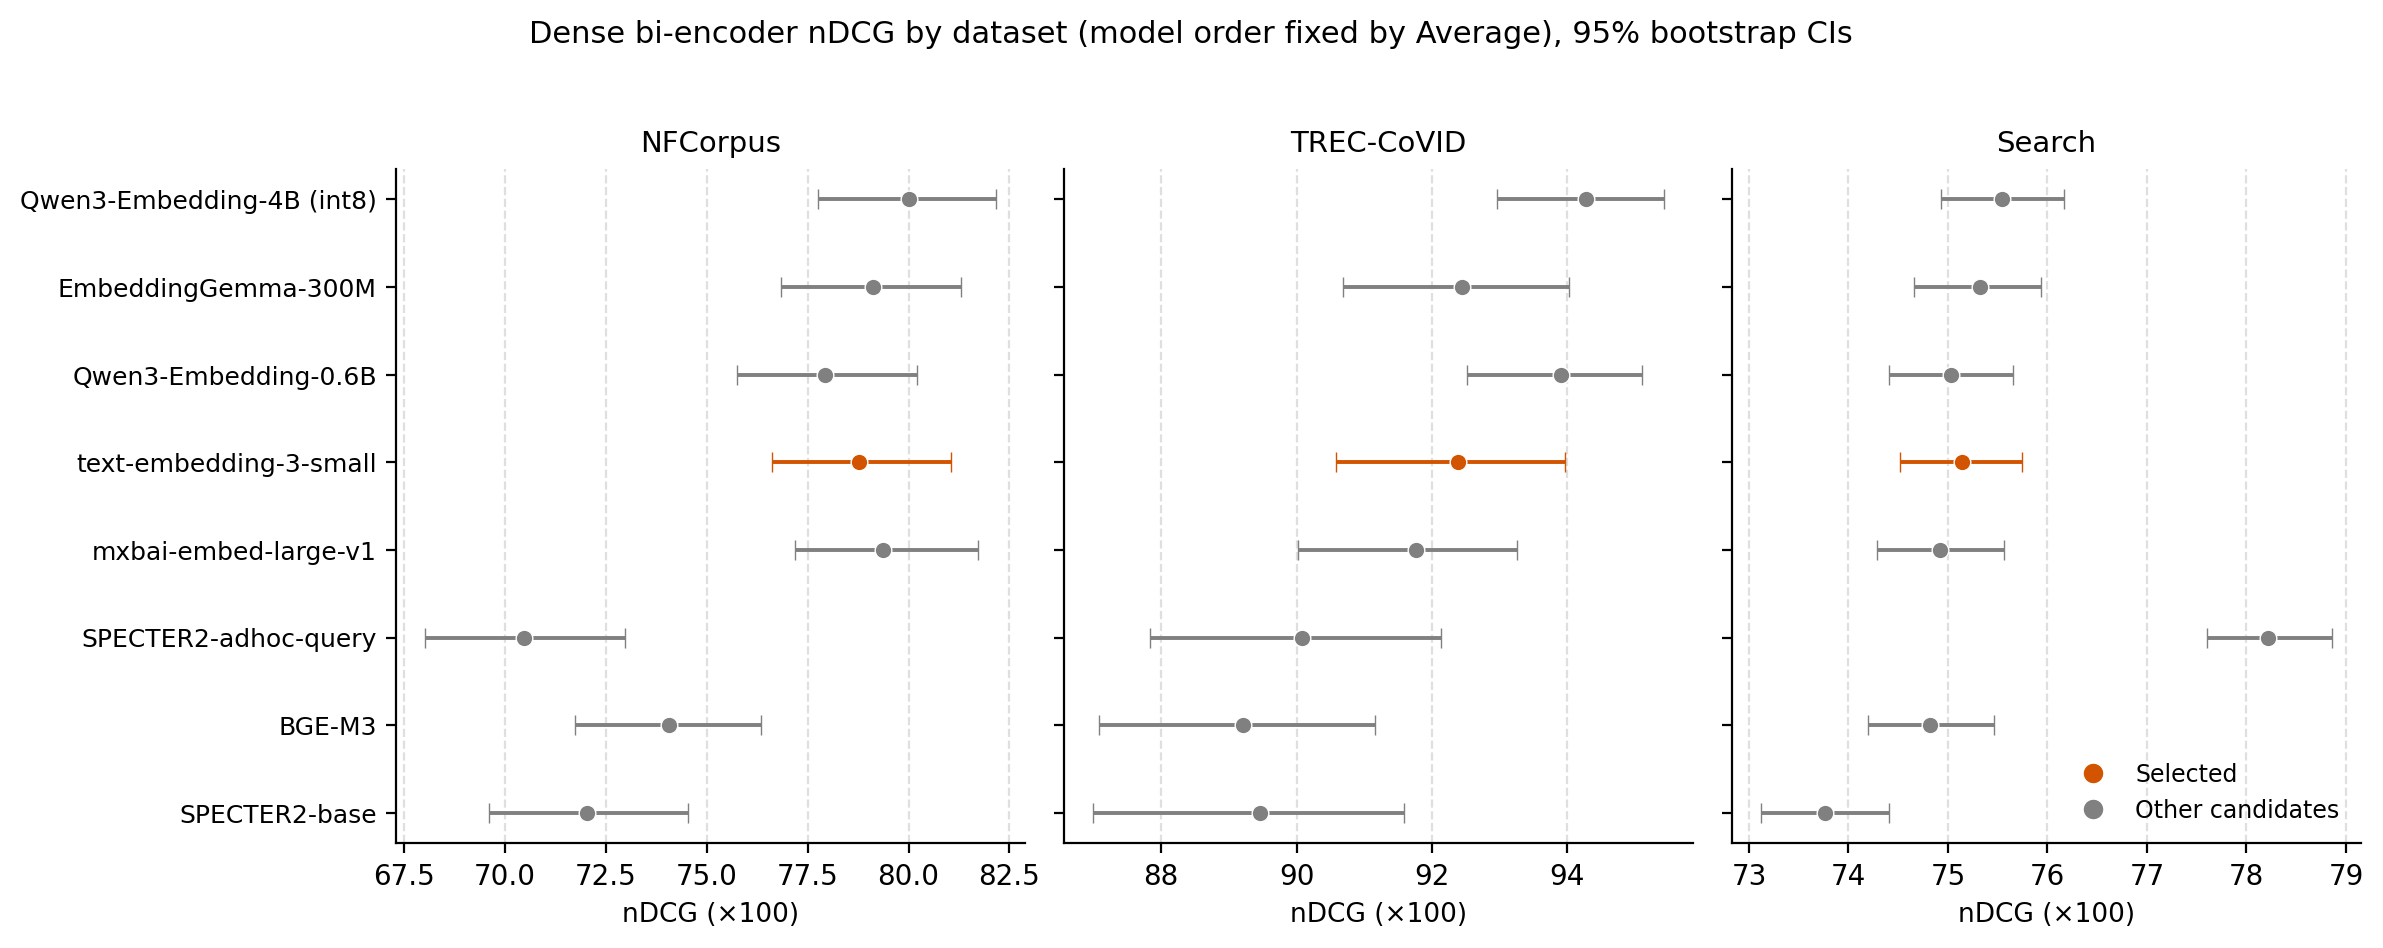
\includegraphics[width=\columnwidth]{images/data_and_results/biencoder_by_dataset.png}
\caption{Dense bi-encoder nDCG on each SciRepEval ad-hoc search task, with models held in their Average order for comparison and 95 percent bootstrap confidence intervals. The selected model is shown in orange.}
\label{fig:bienc-pertask}
\end{figure}

text-embedding-3-small was selected as the dense bi-encoder. The candidate models were evaluated on the three ad-hoc search tasks of SciRepEval, namely NFCorpus, TREC-CoVID, and Search, scored by nDCG. The figure reported is SciRepEval full-ranking nDCG over a per-query candidate pool rather than BEIR full-corpus nDCG@10, which keeps the stage comparable to the scientific retrieval benchmark established in Section~II-D. All scores are nDCG $\times$100 with 95 percent bootstrap intervals from 1000 resamples.

Table~\ref{tab:bienc-results} reports the per-task and average scores in full, and Figure~\ref{fig:bienc-avg} plots each model's average nDCG with its interval. The selected model records an average of 82.10. Qwen3-Embedding-4B holds the highest point estimate at 83.28, but the intervals of the top five models all overlap, forming a statistical tie that contains text-embedding-3-small along with EmbeddingGemma-300M, Qwen3-Embedding-0.6B, and mxbai-embed-large-v1. A clear margin separates this group from the lower three, SPECTER2-adhoc-query at 79.59, BGE-M3 at 79.36, and SPECTER2-base at 78.42, whose intervals fall below the leading cluster.

The average conceals a difference in where each model does its work, shown per task in Figure~\ref{fig:bienc-pertask}. On NFCorpus and TREC-CoVID the general-purpose embedders lead, with Qwen3-Embedding-4B highest on both. On Search the order changes. SPECTER2-adhoc-query scores 78.22 against a field clustered near 75, and this is the single between-model gap on any one task whose interval clears the general models. The same model is weakest on NFCorpus at 70.46, so its Search lead does not survive into the average. The selected model sits within the leading group on each of the three tasks.

\begin{table*}[t]
\caption{Deployment characteristics of the candidate bi-encoders.}
\label{tab:bienc-deploy}
\centering
\footnotesize
\begin{tabular}{@{}lllll@{}}
\toprule
Model & Params (approx.) & Embedding dim & Precision & Self-hostable \\
\midrule
Qwen3-Embedding-4B & $\sim$4 B & 2560 & int8 & yes \\
EmbeddingGemma-300M & $\sim$300 M & 768 & fp16 & yes \\
Qwen3-Embedding-0.6B & $\sim$0.6 B & 1024 & fp16 & yes \\
text-embedding-3-small & undisclosed & 1536 & n/a & no (paid API) \\
mxbai-embed-large-v1 & $\sim$335 M & 1024 & fp16 & yes \\
SPECTER2-adhoc-query & $\sim$110 M & 768 & fp16 & yes \\
BGE-M3 & $\sim$568 M & 1024 & fp16 & yes \\
SPECTER2-base & $\sim$110 M & 768 & fp16 & yes \\
\bottomrule
\end{tabular}

\vspace{3pt}
\begin{minipage}{\linewidth}
\footnotesize\itshape
In-memory footprint per stored vector scales with embedding dimension at int8, at roughly one byte per dimension, giving around 65 GB at 768 dimensions, 87 GB at 1024, 131 GB at 1536, and 218 GB at 2560 over the 85 million works. Encoding cost scales with parameter count.
\end{minipage}
\end{table*}

Table~\ref{tab:bienc-deploy} records the deployment characteristics that the nDCG scores do not, namely approximate parameter count, embedding dimension, precision, and whether the model is self-hostable. In-memory footprint per stored vector scales with embedding dimension at int8, from around 65 GB at 768 dimensions to around 218 GB at 2560 dimensions over the 85 million works, while encoding cost scales with parameter count. The selected model has an embedding dimension of 1536, placing its footprint at around 131 GB, and is served through a paid API rather than self-hosted.

% ----------------------------------------------------------------------------
\subsection{Cross-encoder Re-ranking}

\begin{table*}[t]
\caption{Cross-encoder re-ranking on SciRepEval ad-hoc search, nDCG $\times$100 with 95 percent bootstrap confidence intervals, sorted by Average.}
\label{tab:xenc-results}
\centering
\scriptsize
\setlength{\tabcolsep}{4pt}
\begin{tabular}{@{}p{3.2cm}llll@{}}
\toprule
Model (scorer) & NFCorpus & TREC-CoVID & Search & Average \\
\midrule
Cohere Rerank 4.0 Pro (API) & \textbf{80.42 [78.17, 82.60]} & \textbf{94.60 [93.30, 95.71]} & 75.39 [74.76, 76.00] & \textbf{83.47 [82.54, 84.33]} \\
Qwen3-Reranker-4B (int8) & 80.10 [77.94, 82.14] & 94.37 [92.90, 95.60] & 74.93 [74.32, 75.56] & 83.13 [82.18, 83.99] \\
Cohere Rerank 4.0 Fast (API) & 78.77 [76.55, 80.98] & 94.15 [92.83, 95.31] & \textbf{75.42 [74.75, 76.04]} & 82.78 [81.83, 83.68] \\
Qwen3-Reranker-0.6B (fp16) & 78.06 [75.65, 80.24] & 93.98 [92.59, 95.20] & 75.25 [74.59, 75.85] & 82.43 [81.50, 83.34] \\
mxbai-rerank-large-v1 (435M) & 78.32 [76.08, 80.76] & 91.50 [89.43, 93.33] & 74.78 [74.15, 75.46] & 81.53 [80.48, 82.59] \\
jina-reranker-v2-base (278M) & 76.73 [74.49, 79.01] & 91.84 [90.05, 93.52] & 75.37 [74.73, 75.99] & 81.31 [80.28, 82.30] \\
MedCPT-Cross-Encoder (109M, biomed) & 75.70 [73.21, 78.03] & 88.91 [86.61, 90.97] & 73.97 [73.34, 74.63] & 79.53 [78.40, 80.66] \\
ms-marco-MiniLM-L-6-v2 (22M) & 73.10 [70.78, 75.48] & 88.78 [86.41, 90.90] & 75.21 [74.58, 75.84] & 79.03 [77.90, 80.13] \\
bge-reranker-v2-m3 (568M) & 70.71 [68.31, 73.07] & 90.30 [88.29, 92.18] & 74.40 [73.78, 75.05] & 78.47 [77.37, 79.53] \\
ms-marco-MiniLM-L-12-v2 (33M) & 69.88 [67.41, 72.38] & 87.17 [84.73, 89.52] & 75.09 [74.44, 75.71] & 77.38 [76.17, 78.54] \\
bge-reranker-large (560M) & 66.49 [64.11, 68.85] & 87.27 [84.61, 89.62] & 74.22 [73.59, 74.85] & 76.00 [74.80, 77.16] \\
bge-reranker-base (278M) & 58.75 [56.38, 60.94] & 84.98 [82.12, 87.60] & 72.60 [71.97, 73.24] & 72.11 [70.84, 73.35] \\
gte-reranker-modernbert-base (150M) & 48.88 [46.82, 50.93] & 79.03 [76.40, 81.60] & 69.94 [69.26, 70.60] & 65.95 [64.91, 67.07] \\
\bottomrule
\end{tabular}

\vspace{3pt}
\begin{minipage}{\linewidth}
\footnotesize\itshape
The metric is SciRepEval ad-hoc-search full-ranking nDCG over a reranking pool, not BEIR full-corpus nDCG@10. Confidence intervals are 95 percent bootstrap [2.5 percent, 97.5 percent] over 1000 iterations with seed 42, with the Average resampled independently within each dataset. The intervals are tight on Search, which has 2585 queries, and wide on TREC-CoVID, which has 50, and bold marks the best point estimate per column. The top four models, namely Cohere Pro, Qwen3-Reranker-4B, Cohere Fast, and Qwen3-Reranker-0.6B, have heavily overlapping Average intervals and form a statistical tie, within which the best self-hostable model, Qwen3-Reranker-4B at int8, is tied with Cohere Pro. On Search the small candidate pool saturates every reranker at around 75. For reference, the bi-encoder embeddings without intervals give the best embedder Qwen3-Embedding-4B at 83.28 Average, SPECTER2-adhoc-query at 78.22 on Search, which is above every reranker here, and text-embedding-3-small at 82.10 Average.
\end{minipage}
\end{table*}

\begin{figure}[t]
\centering
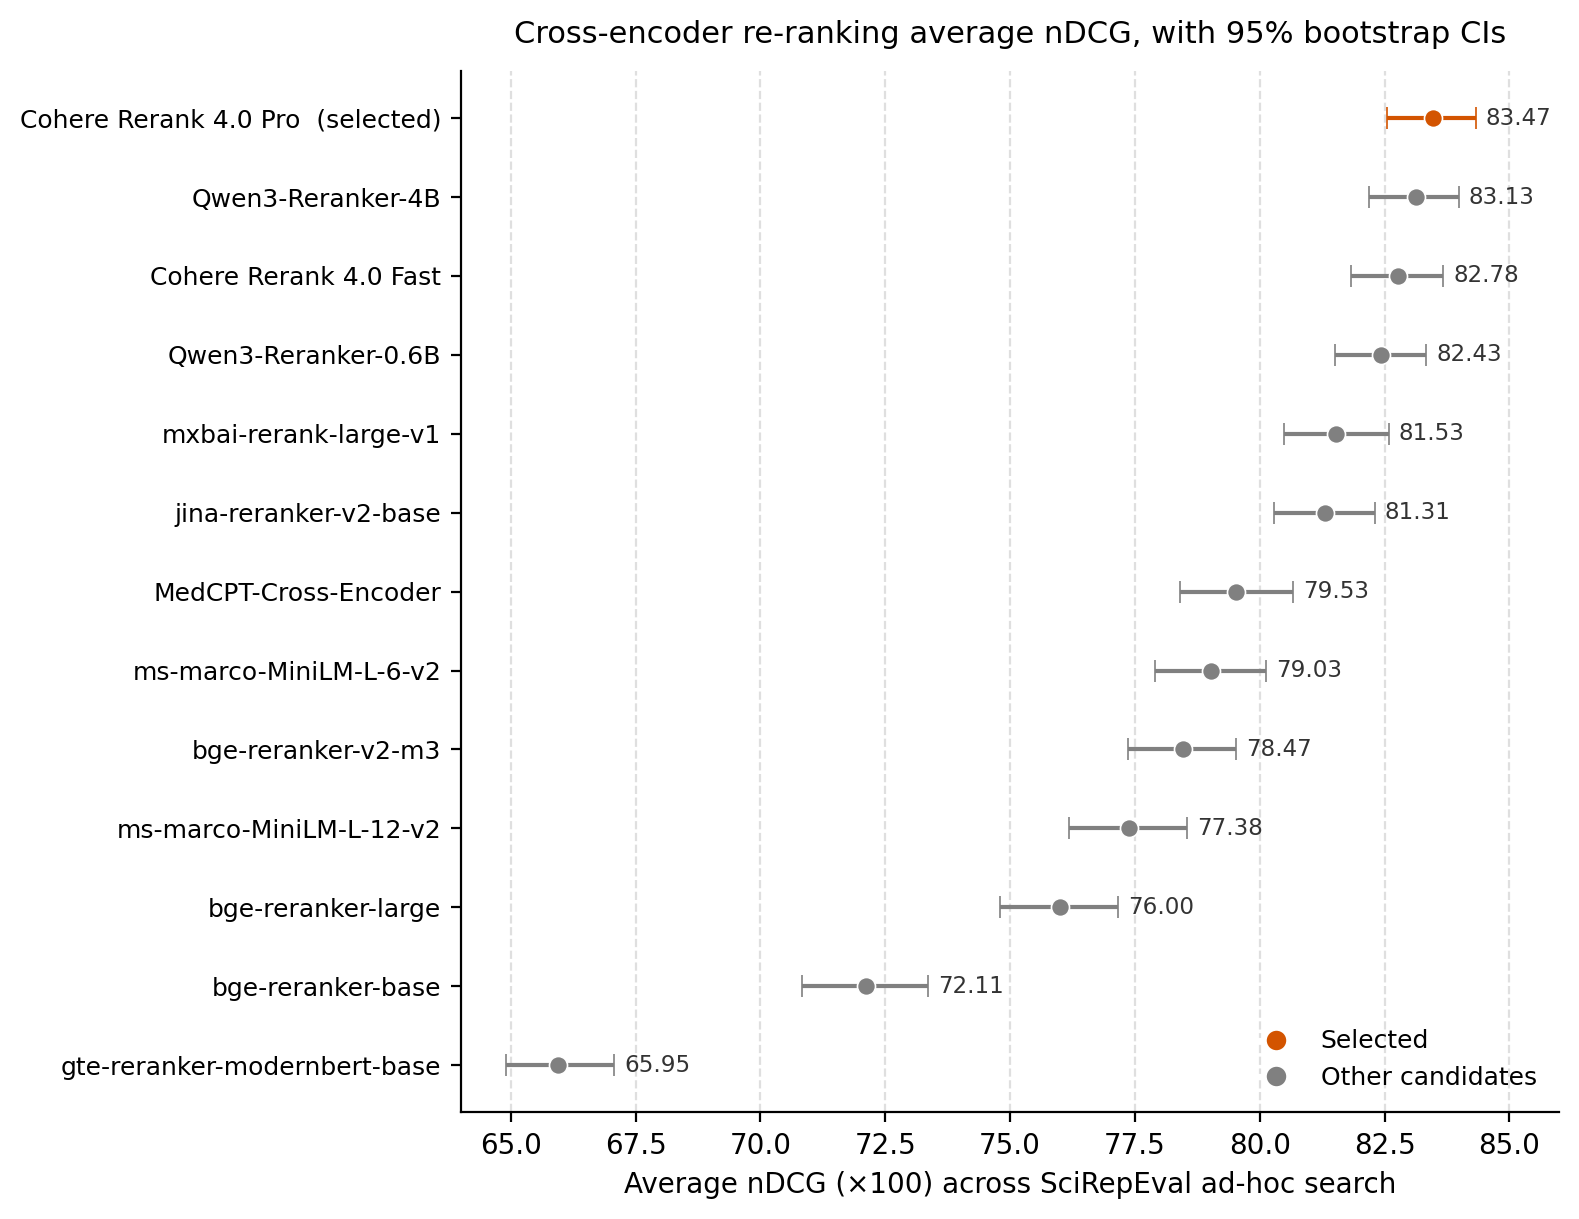
\includegraphics[width=\columnwidth]{images/data_and_results/crossencoder_average.png}
\caption{Cross-encoder re-ranking average nDCG across the three SciRepEval ad-hoc search tasks, with 95 percent bootstrap confidence intervals from 1000 resamples. The selected model is shown in orange.}
\label{fig:xenc-avg}
\end{figure}

\begin{figure}[t]
\centering
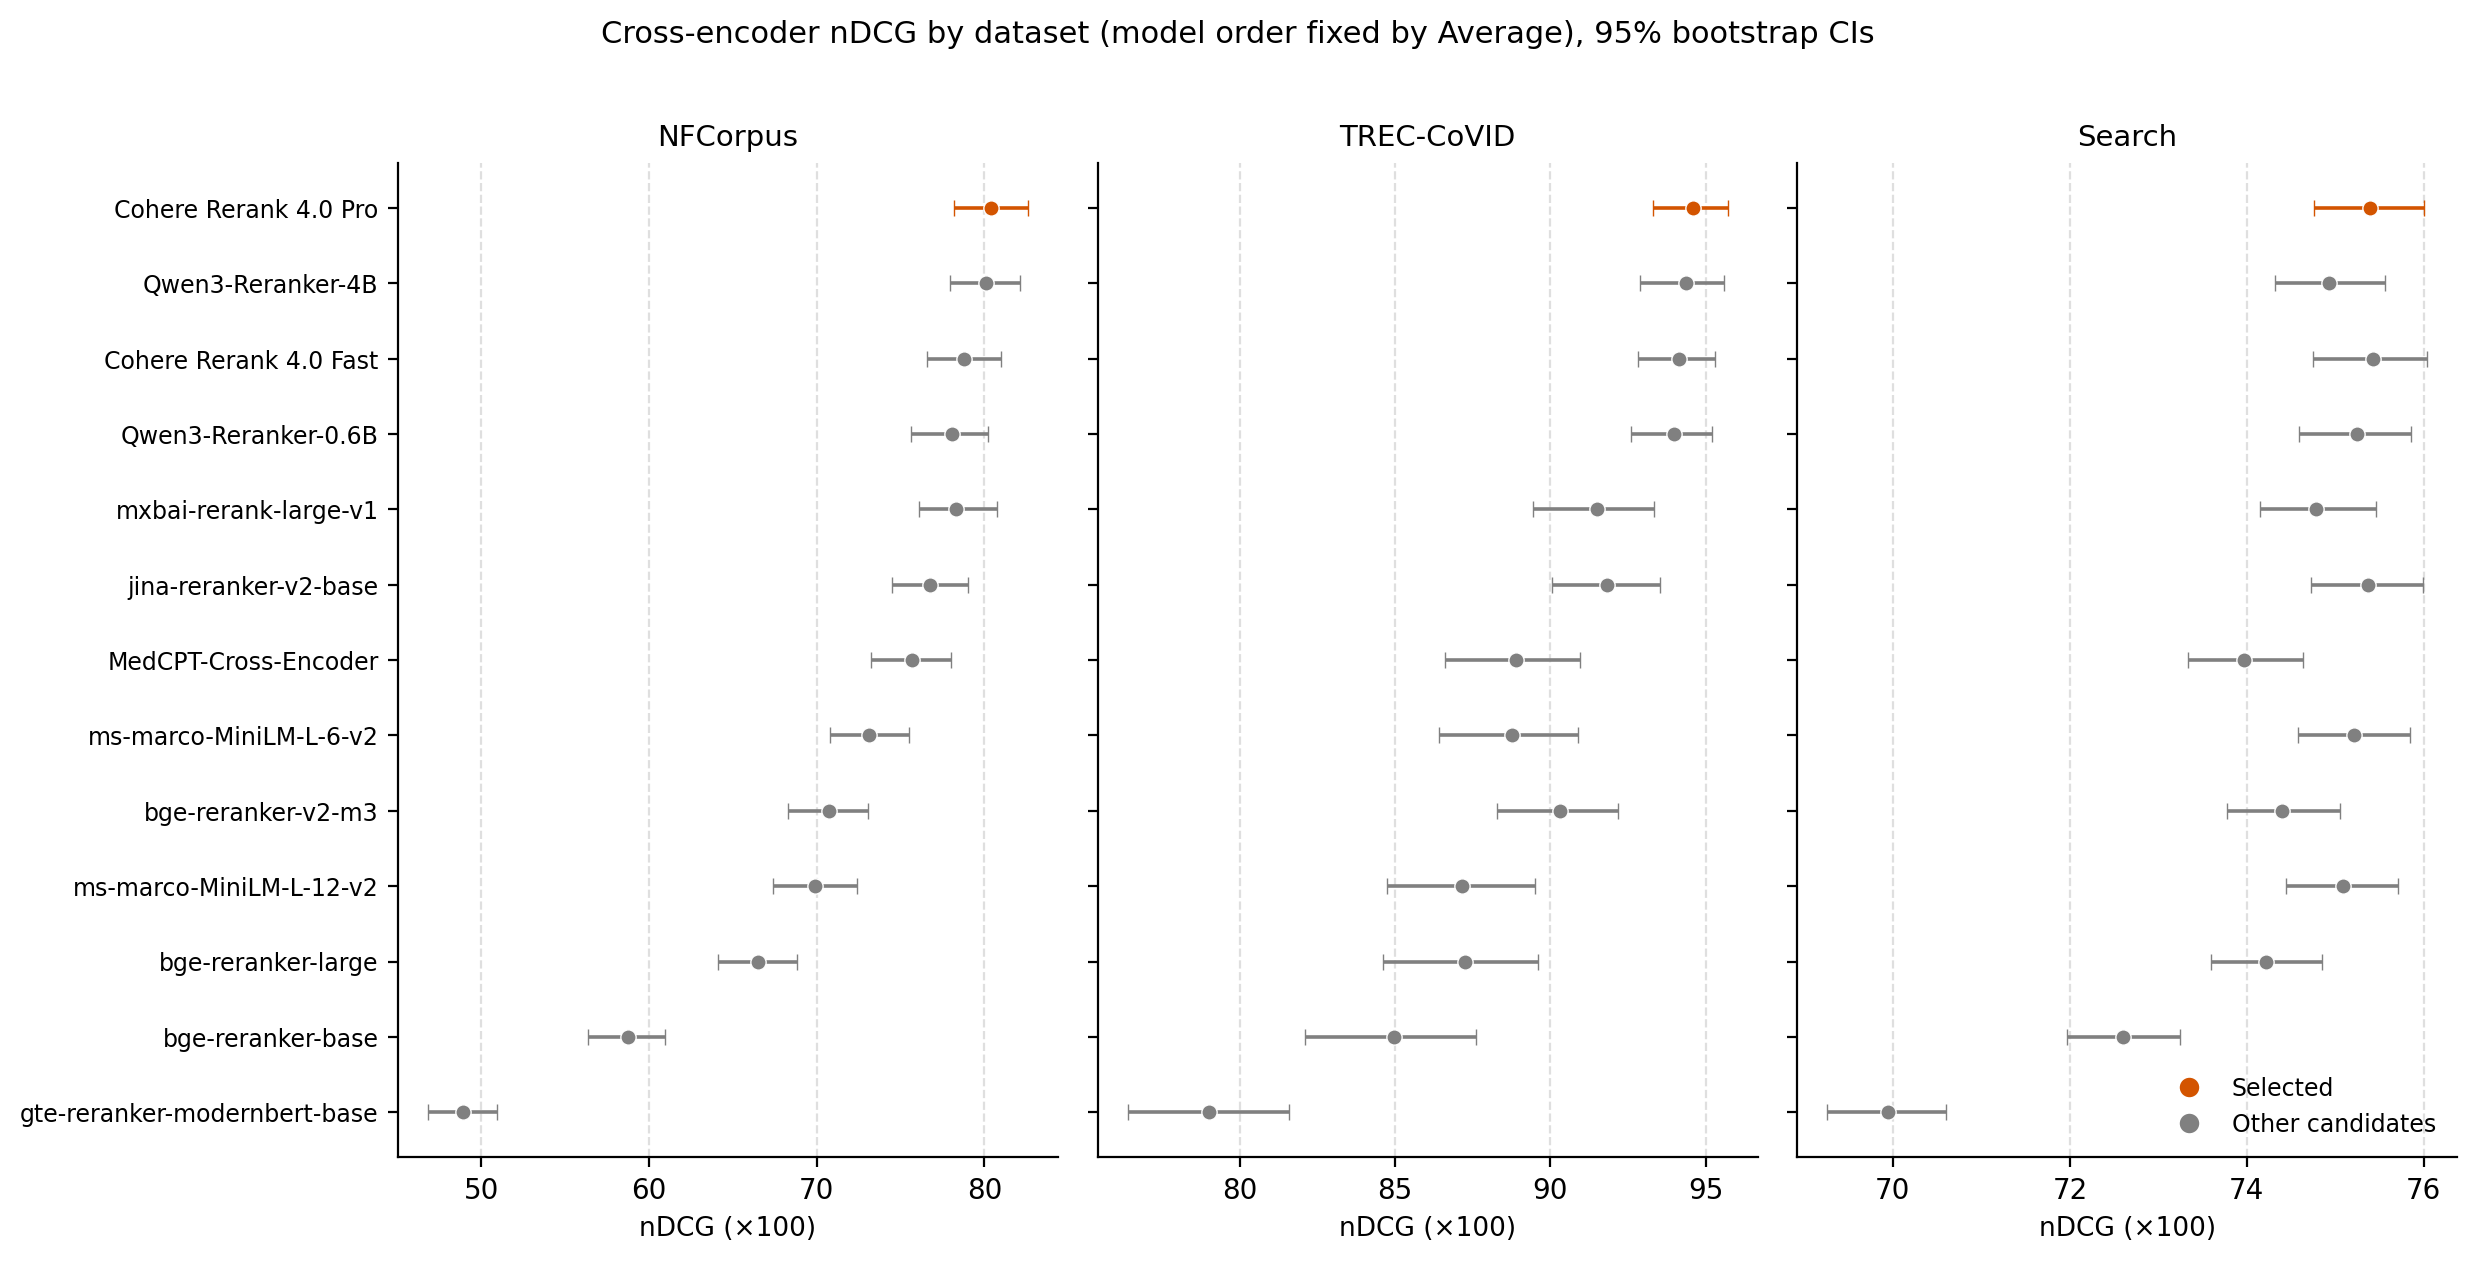
\includegraphics[width=\columnwidth]{images/data_and_results/crossencoder_by_dataset.png}
\caption{Cross-encoder nDCG on each SciRepEval ad-hoc search task, with models held in their Average order for comparison and 95 percent bootstrap confidence intervals. The selected model is shown in orange.}
\label{fig:xenc-pertask}
\end{figure}

Cohere Rerank 4.0 Pro was selected as the cross-encoder. The candidate rerankers were evaluated on the same three SciRepEval ad-hoc search tasks as the bi-encoder and under the same nDCG metric, scoring each model by the ranking it produces when it re-ranks the retrieved candidate pool. All scores are nDCG $\times$100 with 95 percent bootstrap intervals from 1000 resamples. The intervals are tight on Search, which has 2585 queries, and wide on TREC-CoVID, which has 50.

Table~\ref{tab:xenc-results} reports the full per-task and average scores, and Figure~\ref{fig:xenc-avg} plots each model's average with its interval. The selected model holds the highest average at 83.47. Its interval overlaps those of the next three models, Qwen3-Reranker-4B at 83.13, Cohere Rerank 4.0 Fast at 82.78, and Qwen3-Reranker-0.6B at 82.43, so these four form a statistical tie at the top. Within that group the strongest self-hostable model, Qwen3-Reranker-4B, is tied with the selected model. Below the leading four the field descends steadily through a long tail to gte-reranker-modernbert-base at 65.95, a spread of more than seventeen points from top to bottom.

The per-task view in Figure~\ref{fig:xenc-pertask} shows that almost all of this separation comes from NFCorpus, where the models spread across more than thirty points, from 80.42 at the top down to 48.88. Search behaves in the opposite way. Every reranker scores close to 75, since the small candidate pool the stage re-ranks leaves little room to reorder, so the task barely separates the models. TREC-CoVID falls between the two, with a high but noisy spread that reflects its fifty queries.

\begin{table*}[t]
\caption{Deployment characteristics of the candidate cross-encoders.}
\label{tab:xenc-deploy}
\centering
\footnotesize
\begin{tabular}{@{}p{4.5cm}llp{4.0cm}@{}}
\toprule
Model & Params (approx.) & Precision & Self-hostable \\
\midrule
Cohere Rerank 4.0 Pro & undisclosed & n/a & no (paid API) \\
Qwen3-Reranker-4B & $\sim$4 B & int8 & yes (Apache-2.0) \\
Cohere Rerank 4.0 Fast & undisclosed & n/a & no (paid API) \\
Qwen3-Reranker-0.6B & $\sim$0.6 B & fp16 & yes (Apache-2.0) \\
mxbai-rerank-large-v1 & $\sim$435 M & fp16 & yes \\
jina-reranker-v2-base & $\sim$278 M & fp16 & weights CC-BY-NC (non-commercial) \\
MedCPT-Cross-Encoder & $\sim$109 M & fp16 & yes \\
ms-marco-MiniLM-L-6-v2 & $\sim$22 M & fp16 & yes \\
bge-reranker-v2-m3 & $\sim$568 M & fp16 & yes \\
ms-marco-MiniLM-L-12-v2 & $\sim$33 M & fp16 & yes \\
bge-reranker-large & $\sim$560 M & fp16 & yes \\
bge-reranker-base & $\sim$278 M & fp16 & yes \\
gte-reranker-modernbert-base & $\sim$150 M & fp16 & yes \\
\bottomrule
\end{tabular}

\vspace{3pt}
\begin{minipage}{\linewidth}
\footnotesize\itshape
Unlike the bi-encoder, a reranker stores no vectors, so its cost is latency, which scales with parameter count, rather than memory, which is why the stage runs over only around 100 candidates. The Qwen3 rerankers are released under Apache-2.0, while the jina-reranker-v2 weights are CC-BY-NC-4.0 and so are non-commercial and not deployable in a commercial product. The remaining licences should be confirmed against the deployment terms before selection.
\end{minipage}
\end{table*}

Table~\ref{tab:xenc-deploy} records the deployment characteristics, namely approximate parameter count, precision, and whether the model is self-hostable along with its licence. Unlike the bi-encoder, a reranker stores no vectors, so its cost is latency rather than memory and scales with parameter count, which is the reason the stage runs over only around 100 candidates. The self-hostable options carry mixed licences, with the Qwen3 rerankers released under Apache-2.0 and the jina reranker under a non-commercial CC-BY-NC licence, while the selected model is served through a paid API.

% ----------------------------------------------------------------------------
\subsection{Embedding Quantisation}
% Placeholder. Results not yet available.
\textit{[Placeholder. Results comparing int8 against full-precision nDCG, and the resulting accuracy cost, to be added.]}

% ----------------------------------------------------------------------------
\subsection{System-Level Evaluation}
% Placeholder. Results not yet available.
\textit{[Placeholder. End-to-end results over a realistic query set with light relevance judgments to be added.]}   (or \include{...})
%
%  Requires in the preamble of main.tex:
%      \usepackage{booktabs}
%      \usepackage{graphicx}
%      \usepackage{array}      % only if you later add >{...} column types
%
%  Figures use placeholder paths under figures/ -- replace with your exports.
%  Tables and figures are referenced with \ref so numbering stays dynamic and
%  any table can be moved to an appendix without breaking the prose.
% ============================================================================

\section{Data and Results}

This section reports the result of each component benchmark from the validation design in Section~II-D, taking the components in turn.

% ----------------------------------------------------------------------------
\subsection{Keyword Generation}

\begin{table}[t]
\caption{KPBiomed keyword extraction, present and absent F1@5 with stemming. Models are ordered by present F1, and GPT-5.4-nano is the deployed model.}
\label{tab:kw-kpbiomed}
\centering
\footnotesize
\begin{tabular}{@{}lrr@{}}
\toprule
Model & Present F1@5 & Absent F1@5 \\
\midrule
\textbf{GPT-5.4-nano} & \textbf{30.86} & 1.95 \\
MultipartiteRank & 19.58 & 0.00 \\
TF-IDF & 18.56 & 0.04 \\
KeyBART & 17.40 & \textbf{2.07} \\
YAKE & 16.79 & 0.02 \\
KBIR-inspec & 16.36 & 0.01 \\
KeyBERT-MiniLM & 8.52 & 0.04 \\
TextRank & 5.11 & 0.00 \\
\bottomrule
\end{tabular}
\end{table}

\begin{figure*}[t]
\centering
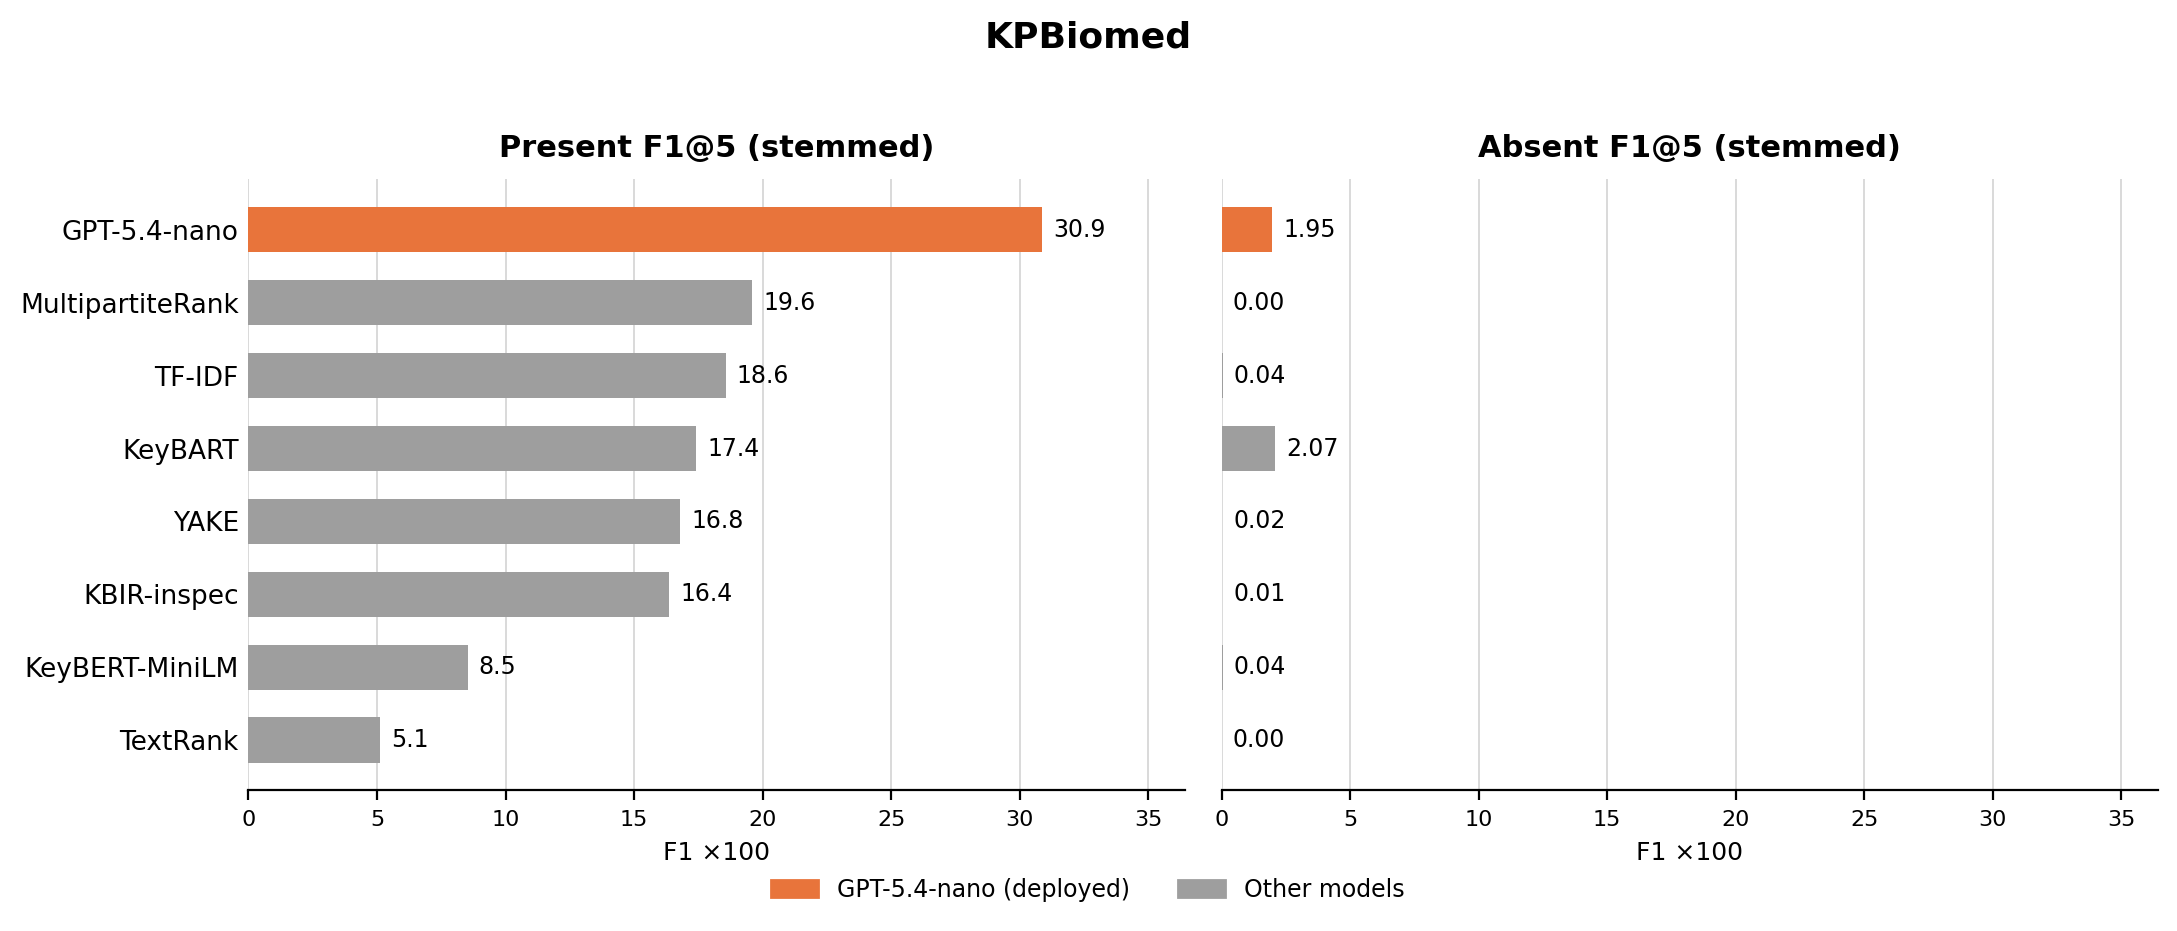
\includegraphics[width=\textwidth]{images/data_and_results/keyword_kpbiomed.png}
\caption{KPBiomed keyword extraction, present and absent F1@5 by model with stemming. The deployed model GPT-5.4-nano is shown in orange and the remaining baselines in grey.}
\label{fig:kw-kpbiomed}
\end{figure*}

\begin{table}[t]
\caption{OAGKX keyword extraction, present and absent F1@5 with stemming. Models are ordered by present F1, and GPT-5.4-nano is the deployed model.}
\label{tab:kw-oagkx}
\centering
\footnotesize
\begin{tabular}{@{}lrr@{}}
\toprule
Model & Present F1@5 & Absent F1@5 \\
\midrule
KeyBART & \textbf{28.42} & \textbf{5.09} \\
\textbf{GPT-5.4-nano} & 26.49 & 1.77 \\
KBIR-inspec & 20.16 & 0.05 \\
MultipartiteRank & 18.83 & 0.00 \\
TF-IDF & 15.55 & 0.03 \\
KeyBERT-MiniLM & 12.04 & 0.04 \\
TextRank & 11.15 & 0.02 \\
YAKE & 8.85 & 0.00 \\
\bottomrule
\end{tabular}
\end{table}

\begin{figure*}[t]
\centering
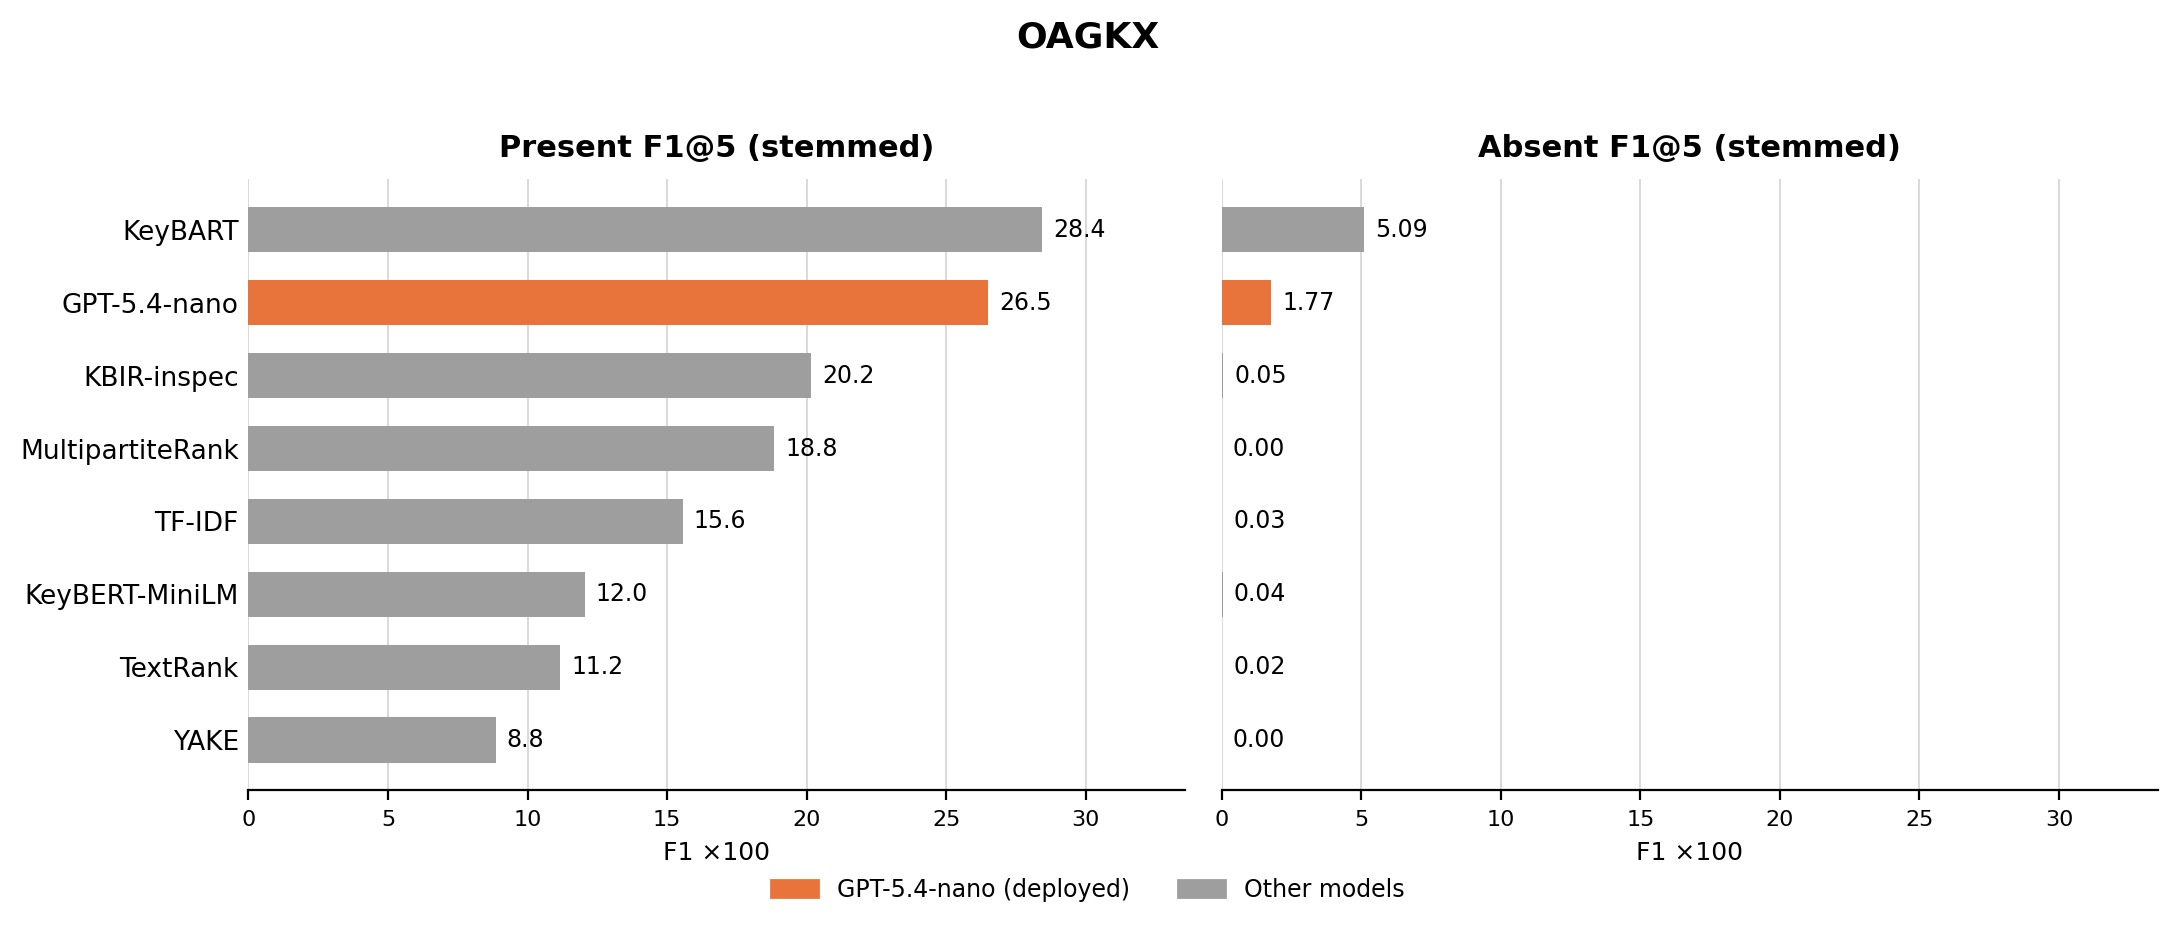
\includegraphics[width=\textwidth]{images/data_and_results/keyword_oagkx.png}
\caption{OAGKX keyword extraction, present and absent F1@5 by model with stemming. The deployed model GPT-5.4-nano is shown in orange and the remaining baselines in grey.}
\label{fig:kw-oagkx}
\end{figure*}

\begin{table}[t]
\caption{PubMedAKE keyword extraction, present and absent F1@5 with stemming. Models are ordered by present F1, and GPT-5.4-nano is the deployed model.}
\label{tab:kw-pubmedake}
\centering
\footnotesize
\begin{tabular}{@{}lrr@{}}
\toprule
Model & Present F1@5 & Absent F1@5 \\
\midrule
\textbf{GPT-5.4-nano} & \textbf{36.44} & \textbf{1.30} \\
TF-IDF & 24.06 & 0.03 \\
MultipartiteRank & 23.06 & 0.00 \\
KBIR-inspec & 19.36 & 0.01 \\
KeyBART & 18.41 & 1.29 \\
YAKE & 12.92 & 0.01 \\
KeyBERT-MiniLM & 6.78 & 0.01 \\
TextRank & 4.68 & 0.00 \\
\bottomrule
\end{tabular}
\end{table}

\begin{figure*}[t]
\centering
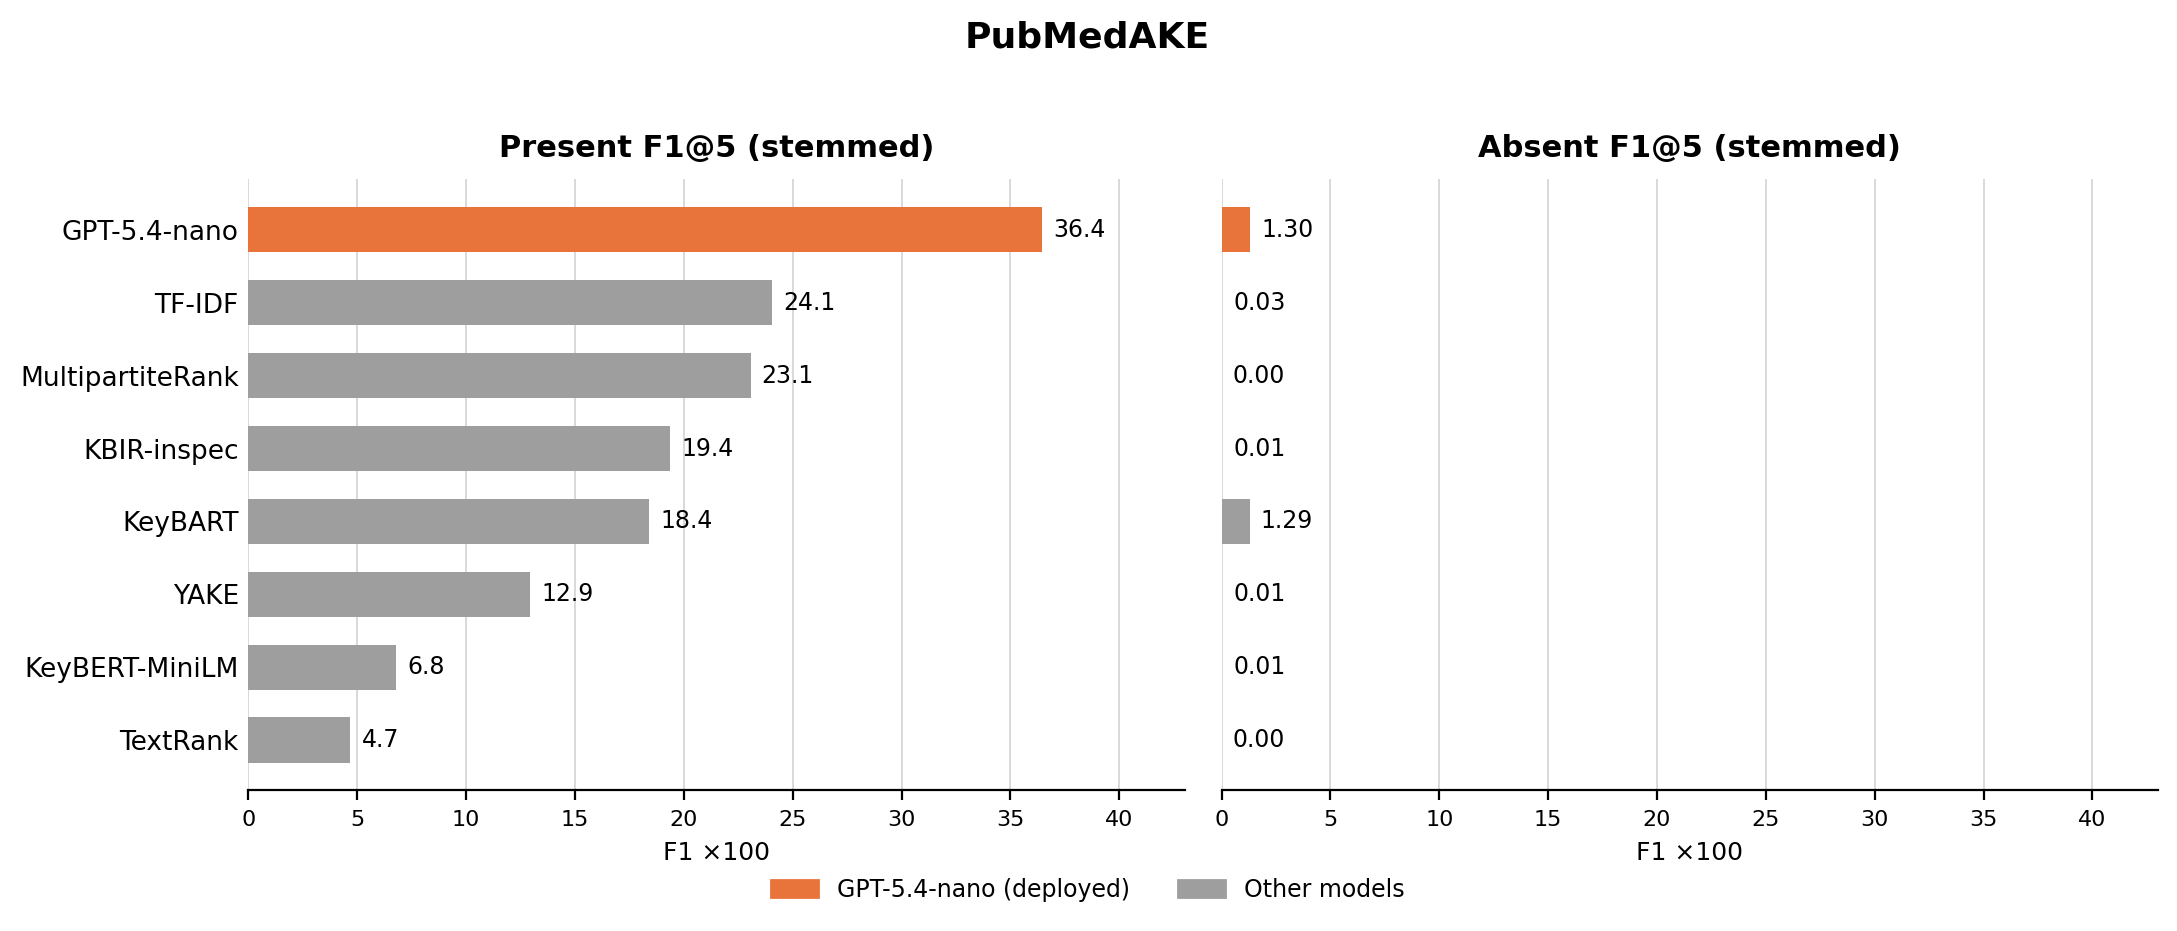
\includegraphics[width=\textwidth]{images/data_and_results/keyword_pubmedake.png}
\caption{PubMedAKE keyword extraction, present and absent F1@5 by model with stemming. The deployed model GPT-5.4-nano is shown in orange and the remaining baselines in grey.}
\label{fig:kw-pubmedake}
\end{figure*}

GPT-5.4-nano was benchmarked for keyword generation against a set of statistical and neural baselines on KPBiomed, OAGKX, and PubMedAKE. Tables~\ref{tab:kw-kpbiomed} to~\ref{tab:kw-pubmedake} report the results for each dataset in turn. Throughout, present (extractive) keyphrases, which occur verbatim in the source text, are distinguished from absent (abstractive) keyphrases, which do not and so must be generated. Matches are scored by F1 at five with light stemming, so that a keyphrase and its stem count as a match while a different word of the same meaning does not.

On the present keyphrase tasks, GPT-5.4-nano records the highest score on KPBiomed and PubMedAKE and the second highest on OAGKX, where KeyBART leads. Its margin is widest on PubMedAKE, at 36.44 against a next-best of 24.06.

On the absent keyphrase tasks, which a model can only score on by producing keyphrases that do not occur in the source text, GPT-5.4-nano scores in the low single digits, from 1.30 on PubMedAKE to 1.95 on KPBiomed. These non-zero scores indicate that the model generates a small portion of its keyphrases rather than extracting all of them. The other generative baseline, KeyBART, behaves similarly and records the highest absent score on KPBiomed and OAGKX. The statistical extractors such as TF-IDF, YAKE, TextRank, and MultipartiteRank remain near zero here, since they return only spans found in the source text and so do not generate at all.

\begin{table}[t]
\caption{Keyword extraction stability for GPT-5.4-nano over three runs on a 2000-document sample.}
\label{tab:kw-stability}
\centering
\footnotesize
\begin{tabular}{@{}p{0.66\columnwidth}r@{}}
\toprule
Quantity & Value \\
\midrule
Set-level Jaccard across runs & 0.73 \\
Present-F1 run-to-run std & $\pm$0.07 \\
Deterministic baselines (TF-IDF, YAKE, TextRank, MultipartiteRank, KeyBERT, KBIR) & 1.00 \\
\bottomrule
\end{tabular}
\end{table}

Table~\ref{tab:kw-stability} reports a reproducibility check for GPT-5.4-nano over three runs on a 2000-document sample. The set-level Jaccard similarity across runs is 0.73, meaning that for a given document around 73 percent of the combined set of keyphrases from any two runs is shared by both, equivalent to roughly one in six keyphrases changing between runs. The model is therefore largely repeatable but not deterministic, unlike the baselines, which are reproducible by construction. The effect on measured performance is negligible, with a run-to-run present-F1 standard deviation of 0.07. The same sample also reproduces the full-split figures to within roughly a tenth of a point, confirming that the smaller stability sample does not shift the headline results.

% ----------------------------------------------------------------------------
\subsection{IR Extraction}

\begin{table*}[t]
\caption{Natural-language-to-IR accuracy by model. Joint IR accuracy counts a query as correct when both its entities and its boolean expression are correct under exact matching, reported in the as-deployed or best configuration for each model.}
\label{tab:ir-accuracy}
\centering
\footnotesize
\begin{tabular}{@{}lllcc@{}}
\toprule
Model & Host & Configuration & IR accuracy & 95\% CI \\
\midrule
\textbf{gpt-5.4-nano} & Azure & default, 0 reasoning tok & \textbf{0.937}$^{\dagger}$ & [0.897, 0.983] \\
gpt-5-mini & Azure & default, 384 reasoning tok & 0.931 & [0.879, 0.974] \\
qwen3:8b & Local (Q4) & single-shot & 0.802 & [0.733, 0.871] \\
qwen3:4b & Local (Q4) & thinking$^{\ddagger}$ & 0.784 & [0.707, 0.862] \\
qwen2.5:3b & Local (Q4) & non-reasoning & 0.207 & [0.138, 0.284] \\
phi4-mini & Local (Q4) & non-reasoning & 0.052 & [0.017, 0.095] \\
llama3.2:3b & Local (Q4) & non-reasoning & 0.026 & [0.000, 0.060] \\
\bottomrule
\end{tabular}

\vspace{3pt}
\begin{minipage}{\linewidth}
\footnotesize\itshape
Confidence intervals are 95 percent bootstrap over 1000 iterations. Cross-model gaps that fall within these intervals are treated as ties, and bold marks the deployed model. The dagger denotes a three-run mean, whose single-run range is 0.914 to 0.940, with temperature zero returning a byte-identical output on 96.6 percent of queries (Table~\ref{tab:ir-stability}). The double dagger denotes qwen3:4b, whose single-shot configuration produced degenerate empty output, so its thinking configuration is its only usable score.
\end{minipage}
\end{table*}

\begin{figure}[t]
\centering
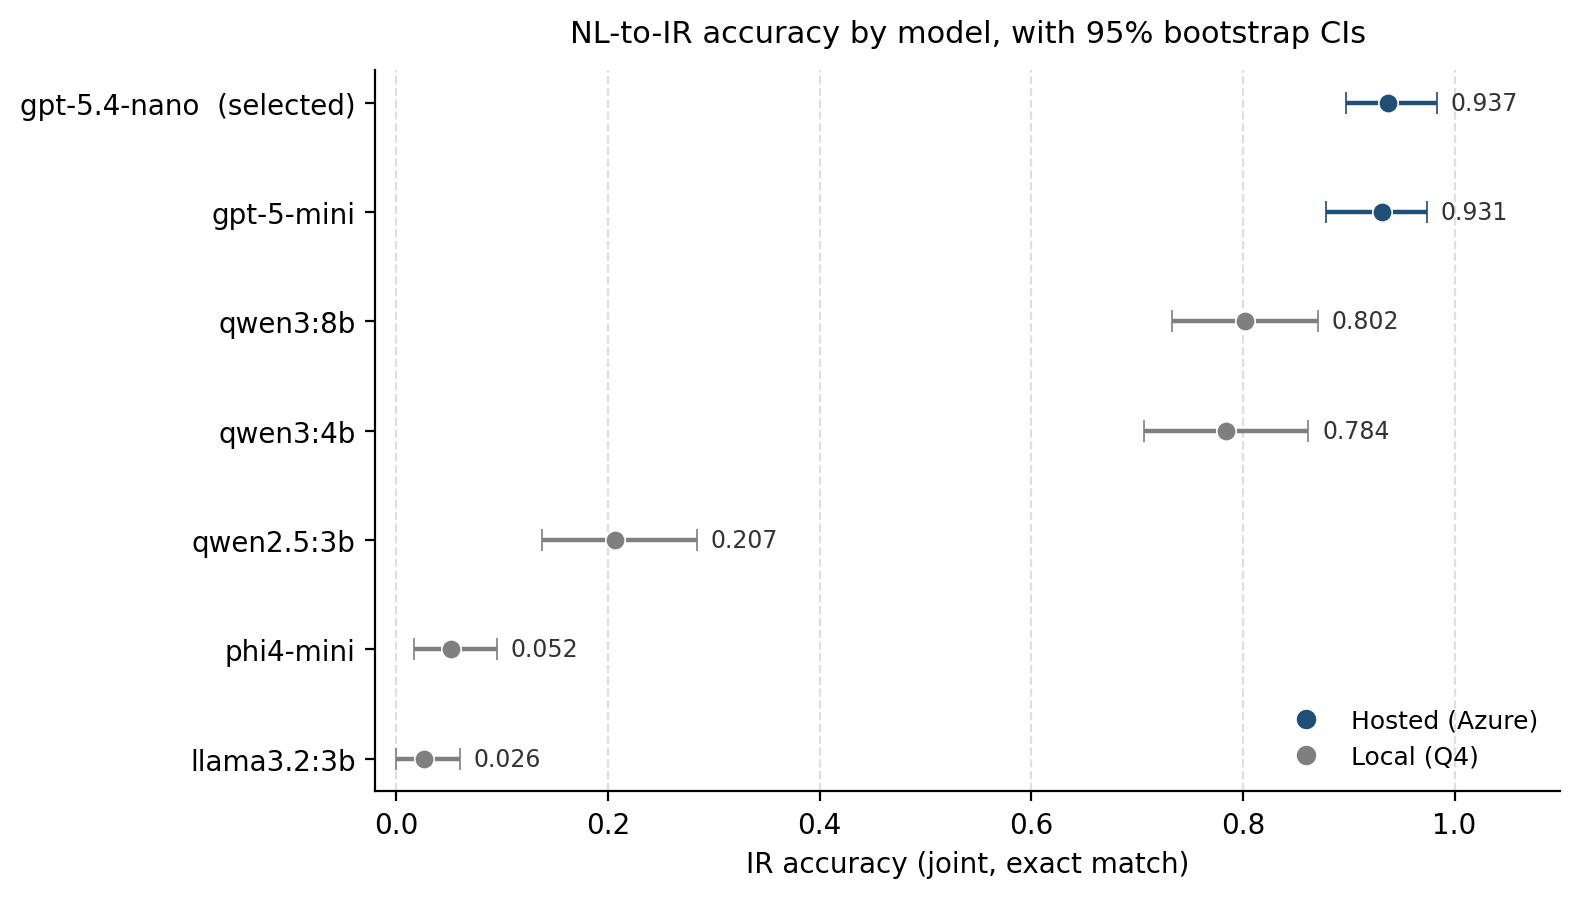
\includegraphics[width=\columnwidth]{images/data_and_results/ir_accuracy_ci.png}
\caption{Natural-language-to-IR joint accuracy by model on the hand-built gold set, with 95 percent bootstrap confidence intervals from 1000 resamples.}
\label{fig:ir-accuracy}
\end{figure}

GPT-5.4-nano was benchmarked for natural-language-to-IR extraction against a set of hosted and local models on a hand-built gold set of queries paired with their correct intermediate representations. The set was constructed to exercise every entity type the system supports across a range of boolean structures, from single topics through to bracketed combinations of AND, OR, and NOT, so that performance on it reflects the input and output behaviour the system actually requires. The headline measure, IR accuracy, is the joint figure reported in Table~\ref{tab:ir-accuracy}, counting a query as correct only when both its extracted entities and its boolean expression are correct under exact matching.

Figure~\ref{fig:ir-accuracy} plots each model's accuracy with its 95 percent bootstrap interval. The two hosted models lead the benchmark by a clear margin, with GPT-5.4-nano highest at an IR accuracy of 0.937 and GPT-5-mini close behind at 0.931. Both hosted intervals clear those of every local model without overlap, placing the hosted advantage beyond sampling noise, while the two overlap each other and are statistically indistinguishable. Among the local models, the two strongest (qwen3:8b and qwen3:4b) reach around 0.80, and the three smaller models fall away sharply to 0.207, 0.052, and 0.026, near the floor of the task.

\begin{table}[t]
\caption{Effect of reasoning on IR accuracy.}
\label{tab:ir-reasoning}
\centering
\footnotesize
\begin{tabular}{@{}lccc@{}}
\toprule
Model & Reasoning off & Reasoning on & $\Delta$ \\
\midrule
gpt-5.4-nano & 0.914 & 0.922 & +0.008 \\
gpt-5-mini & \textbf{0.750} & \textbf{0.940} & \textbf{+0.190} \\
\bottomrule
\end{tabular}

\vspace{3pt}
\begin{minipage}{\linewidth}
\footnotesize\itshape
Reasoning is controlled through the Azure \texttt{reasoning\_effort} setting with tokens accounted. Reasoning on used approximately 246 tokens per query for gpt-5.4-nano and 896 for gpt-5-mini, while reasoning off used none. Reasoning lifts the weaker model in each tier, while the stronger one is already at its ceiling.
\end{minipage}
\end{table}

Table~\ref{tab:ir-reasoning} isolates the effect of reasoning on the two GPT models. GPT-5.4-nano gains almost nothing from it, moving from 0.914 without reasoning to 0.922 with around 246 reasoning tokens, a difference of 0.008, and so reaches its accuracy in a single pass with no reasoning budget. GPT-5-mini behaves differently, scoring only 0.750 without reasoning and rising to 0.940 once reasoning is enabled, at a cost of around 896 reasoning tokens per query. The stronger model is already at its ceiling unaided, whereas the weaker one becomes competitive only by spending a substantial token budget.

\begin{table}[t]
\caption{Deployed model, metric decomposition in the default-effort configuration.}
\label{tab:ir-decomp}
\centering
\footnotesize
\begin{tabular}{@{}lcc@{}}
\toprule
Metric & Value & 95\% CI \\
\midrule
IR accuracy (joint) & 0.937 & [0.897, 0.983] \\
Entity F1 (micro) & 0.984 & [0.969, 0.995] \\
Entity F1 (macro) & 0.982 & [0.967, 0.994] \\
Expression equivalence & 0.931 & [0.888, 0.974] \\
Expression graded & 0.985 & [0.974, 0.995] \\
\bottomrule
\end{tabular}

\vspace{3pt}
\begin{minipage}{\linewidth}
\footnotesize\itshape
Joint accuracy is bounded by expression equivalence, since entity extraction almost never fails on its own.
\end{minipage}
\end{table}

\begin{table}[t]
\caption{Deployed model, accuracy by stratum, ordered hardest first.}
\label{tab:ir-stratum}
\centering
\footnotesize
\begin{tabular}{@{}lrrr@{}}
\toprule
Stratum & $n$ & IR accuracy & failures \\
\midrule
\texttt{filter\_distractor} & 10 & 0.700 & 3 \\
\texttt{multi\_negation} & 10 & 0.800 & 2 \\
\texttt{deep\_nested} & 12 & 0.833 & 2 \\
\texttt{hard\_typing} & 12 & 0.917 & 1 \\
\texttt{single\_concept} & 6 & 1.000 & 0 \\
\texttt{multi\_concept} & 12 & 1.000 & 0 \\
\texttt{exclusion} & 12 & 1.000 & 0 \\
\texttt{nested} & 12 & 1.000 & 0 \\
\texttt{mixed\_entity} & 16 & 1.000 & 0 \\
\texttt{review\_style} & 14 & 1.000 & 0 \\
\bottomrule
\end{tabular}

\vspace{3pt}
\begin{minipage}{\linewidth}
\footnotesize\itshape
The count $n$ is small per stratum, at sixteen or fewer, so the failure counts are a more reliable read than the rate, and the per-stratum 95 percent intervals are wide, for example \texttt{filter\_distractor} at 0.700 is seven of ten.
\end{minipage}
\end{table}

Tables~\ref{tab:ir-decomp} and~\ref{tab:ir-stratum} decompose the chosen model's performance, which is strong across both components and most query types. By component, entity extraction is near-perfect, with a micro F1 of 0.984 and a macro F1 of 0.982, while expression equivalence is lower at 0.931 (a graded variant that credits partially correct expressions reaches 0.985). The joint IR accuracy of 0.937 is therefore bounded by the expression score, since entity extraction almost never fails on its own. By query type, the model is perfect on six of the ten strata, covering single and multiple concepts, exclusions, nesting, mixed entities, and review-style queries. Its errors concentrate in the remaining four. The largest source is \texttt{filter\_distractor}, where three of ten queries fail because the model miscategorises a filter term such as a year or citation bound as a searchable entity. The rest fall on the structurally hardest queries, with two of ten failing on multiple negations, two of twelve on deep nesting, and one of twelve on hard typing. Per-stratum counts are small, at sixteen queries or fewer, so the failure counts are a more reliable read than the rates.

\begin{table}[t]
\caption{Stability of the deployed model over three runs.}
\label{tab:ir-stability}
\centering
\footnotesize
\begin{tabular}{@{}p{0.46\columnwidth}cc@{}}
\toprule
Metric & temp 0 & temp 0.7 \\
\midrule
IR identical across all 3 runs & 0.966 & 0.957 \\
Run-to-run IR-accuracy std & 0.004 & 0.004 \\
Majority-vote@3 vs single run & 0.931 vs 0.940 & 0.940 vs 0.940 \\
\bottomrule
\end{tabular}

\vspace{3pt}
\begin{minipage}{\linewidth}
\footnotesize\itshape
Temperature zero is highly but not perfectly deterministic, and majority voting adds nothing.
\end{minipage}
\end{table}

Table~\ref{tab:ir-stability} reports a stability check over three runs. Although GPT-5.4-nano is not deterministic, at temperature zero it returns an identical IR on 96.6 percent of queries, with a run-to-run accuracy standard deviation of 0.004. Aggregating three runs by majority vote changes nothing, at 0.931 against 0.940 for a single run, so the three-run mean of 0.937 reported in Table~\ref{tab:ir-accuracy} is used throughout.

% ----------------------------------------------------------------------------
\subsection{Dense Bi-encoder Retrieval}

\begin{table*}[t]
\caption{Dense bi-encoder retrieval on SciRepEval ad-hoc search, nDCG $\times$100 with 95 percent bootstrap confidence intervals.}
\label{tab:bienc-results}
\centering
\scriptsize
\setlength{\tabcolsep}{4pt}
\begin{tabular}{@{}p{3.0cm}llll@{}}
\toprule
Model & NFCorpus & TREC-CoVID & Search & Average \\
\midrule
Qwen3-Embedding-4B (int8) & \textbf{80.02 [77.75, 82.17]} & \textbf{94.28 [92.96, 95.43]} & 75.54 [74.93, 76.17] & \textbf{83.28 [82.35, 84.19]} \\
EmbeddingGemma-300M & 79.13 [76.84, 81.29] & 92.45 [90.68, 94.03] & 75.32 [74.66, 75.93] & 82.30 [81.32, 83.31] \\
Qwen3-Embedding-0.6B & 77.94 [75.75, 80.22] & 93.90 [92.52, 95.10] & 75.03 [74.41, 75.65] & 82.29 [81.32, 83.25] \\
text-embedding-3-small (existing) & 78.78 [76.61, 81.05] & 92.38 [90.58, 93.96] & 75.14 [74.52, 75.74] & 82.10 [81.08, 83.05] \\
mxbai-embed-large-v1 & 79.37 [77.19, 81.72] & 91.77 [90.02, 93.25] & 74.92 [74.29, 75.56] & 82.02 [81.06, 82.96] \\
SPECTER2-adhoc-query & 70.46 [68.01, 72.97] & 90.08 [87.84, 92.13] & \textbf{78.22 [77.60, 78.86]} & 79.59 [78.46, 80.71] \\
BGE-M3 & 74.05 [71.72, 76.35] & 89.21 [87.08, 91.16] & 74.82 [74.20, 75.46] & 79.36 [78.29, 80.42] \\
SPECTER2-base (existing) & 72.03 [69.60, 74.54] & 89.46 [86.99, 91.58] & 73.76 [73.12, 74.41] & 78.42 [77.27, 79.58] \\
\bottomrule
\end{tabular}

\vspace{3pt}
\begin{minipage}{\linewidth}
\footnotesize\itshape
The metric is SciRepEval ad-hoc-search full-ranking nDCG over a per-query candidate pool, not BEIR full-corpus nDCG@10. Confidence intervals are 95 percent bootstrap [lo, hi] over 1000 iterations with seed 42, and bold marks the best point estimate per column. On Average the top five models' intervals overlap, a statistical tie, and SPECTER2-adhoc-query's Search lead is the one between-model gap whose interval clears the general models.
\end{minipage}
\end{table*}

\begin{figure}[t]
\centering
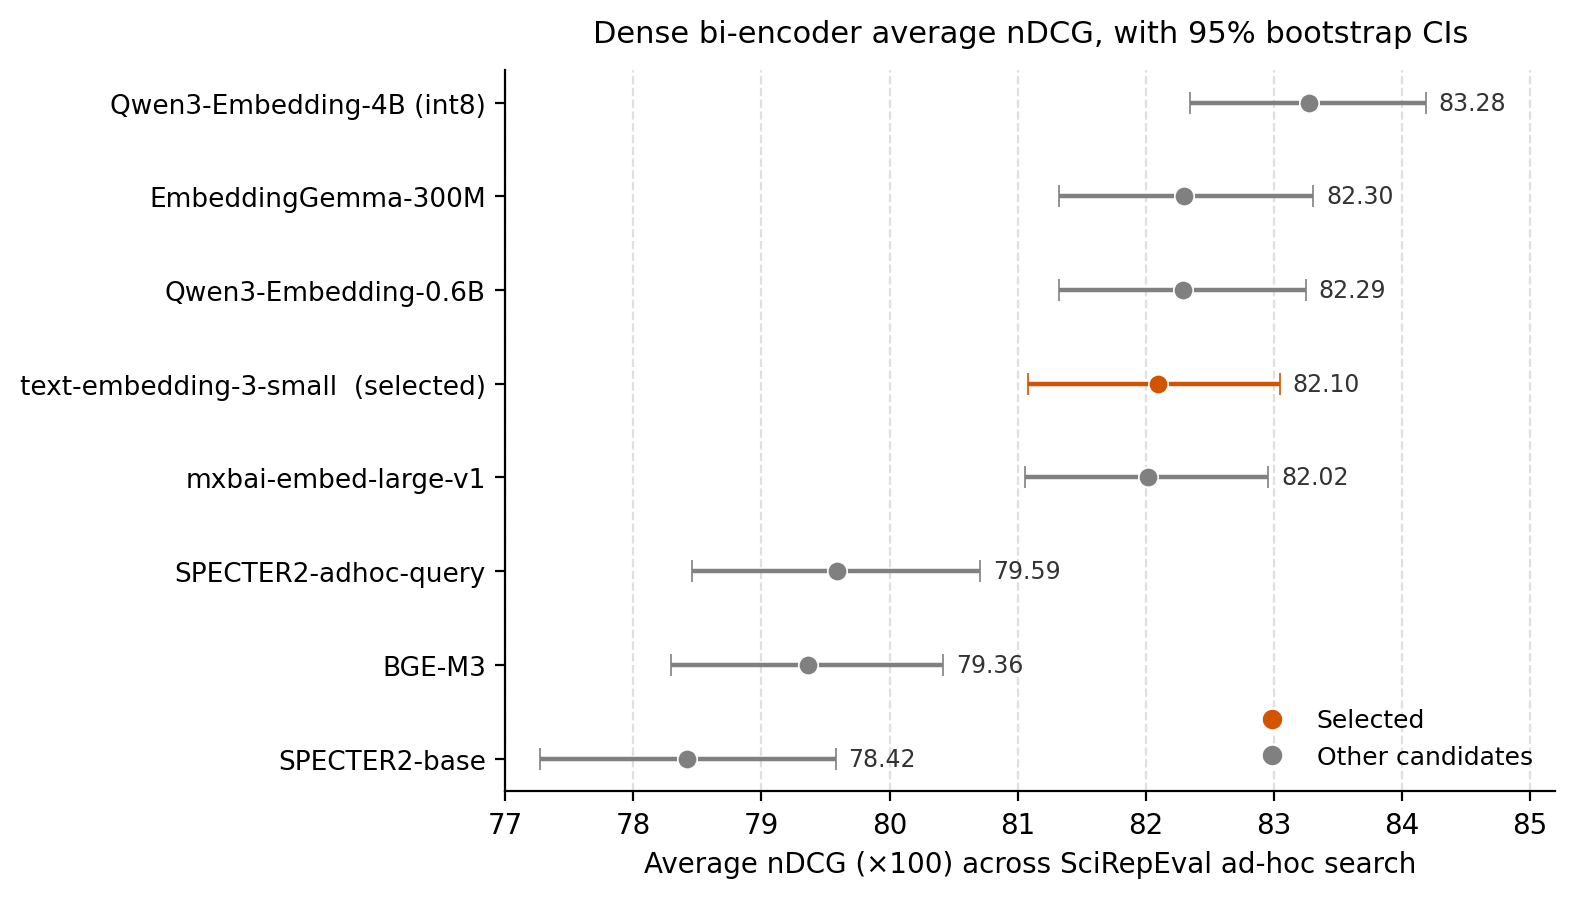
\includegraphics[width=\columnwidth]{images/data_and_results/biencoder_average.png}
\caption{Dense bi-encoder average nDCG across the three SciRepEval ad-hoc search tasks, with 95 percent bootstrap confidence intervals from 1000 resamples. The selected model is shown in orange.}
\label{fig:bienc-avg}
\end{figure}

\begin{figure}[t]
\centering
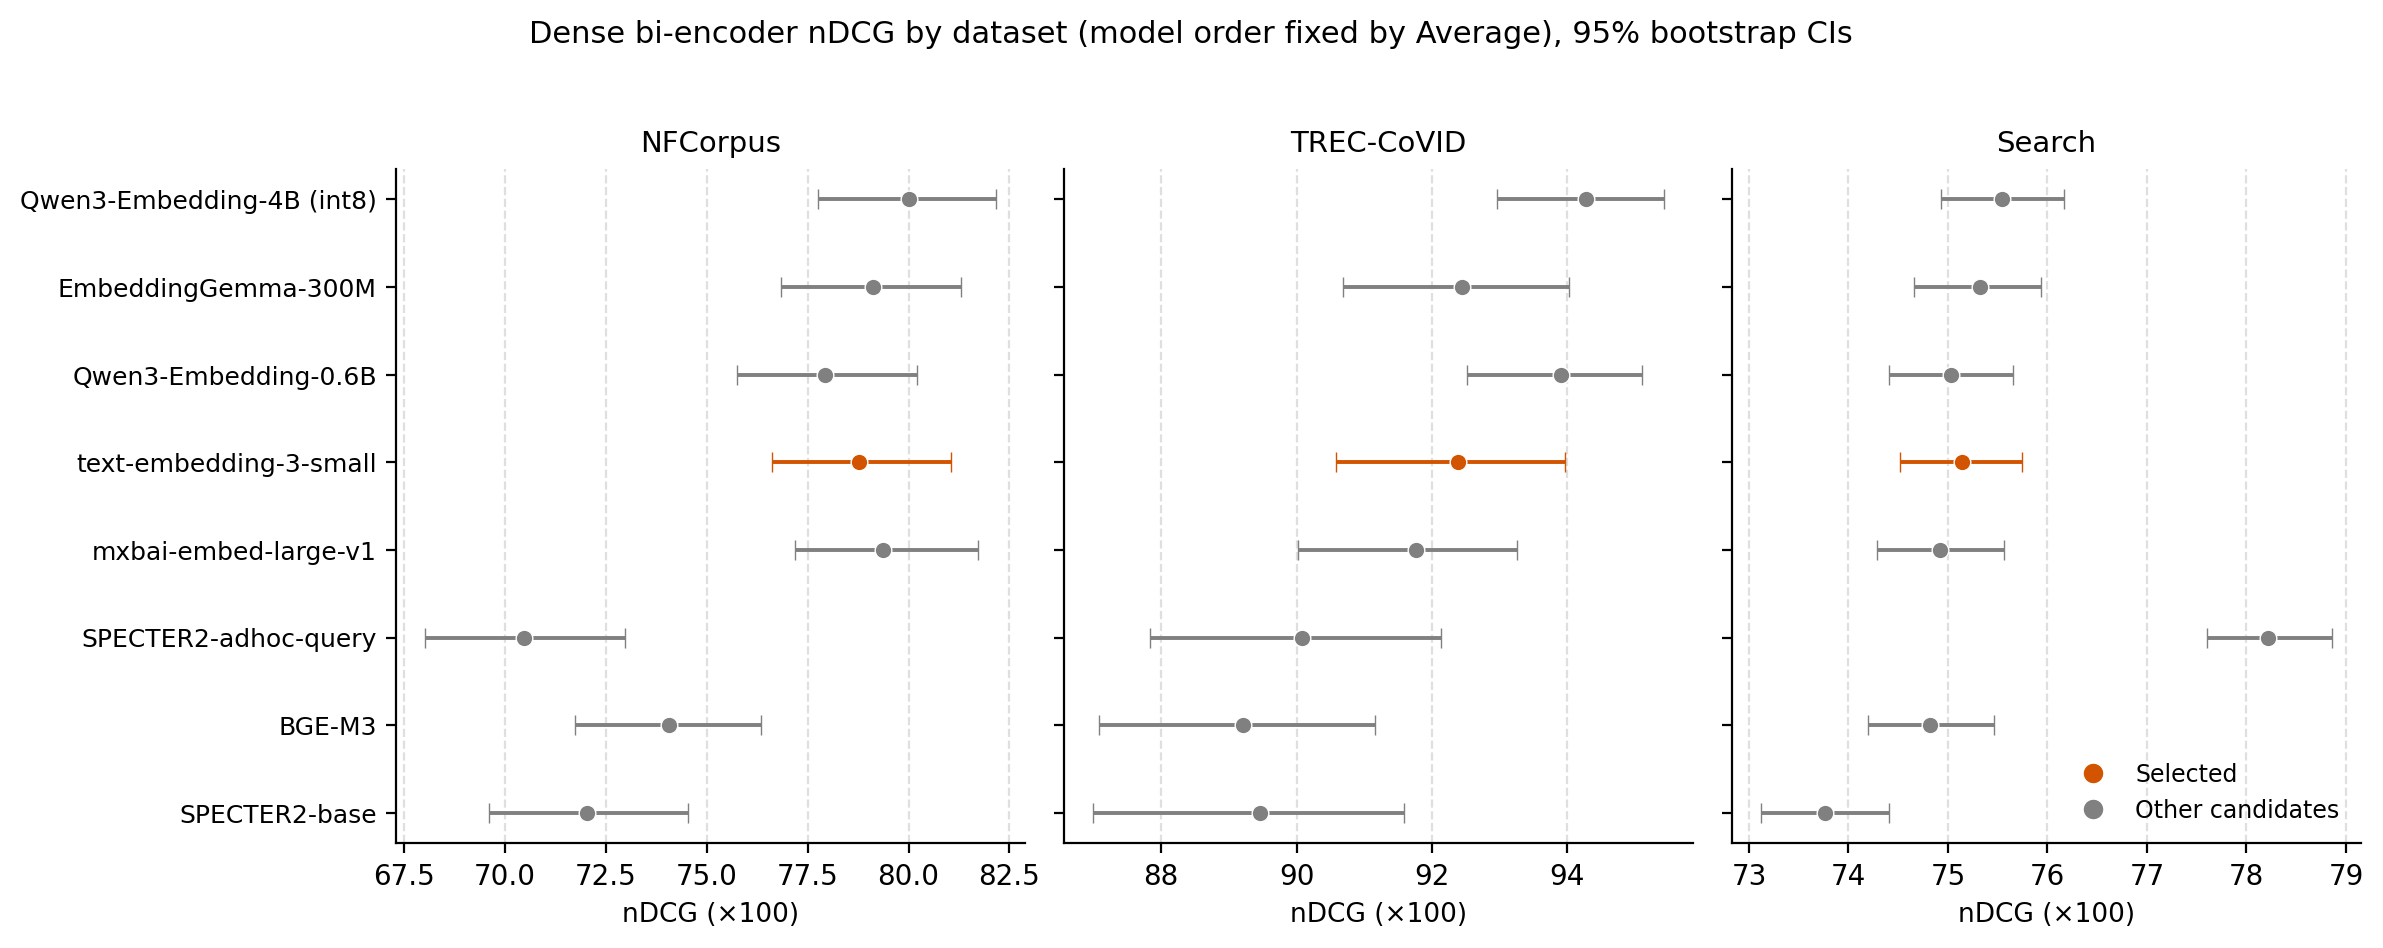
\includegraphics[width=\columnwidth]{images/data_and_results/biencoder_by_dataset.png}
\caption{Dense bi-encoder nDCG on each SciRepEval ad-hoc search task, with models held in their Average order for comparison and 95 percent bootstrap confidence intervals. The selected model is shown in orange.}
\label{fig:bienc-pertask}
\end{figure}

text-embedding-3-small was selected as the dense bi-encoder. The candidate models were evaluated on the three ad-hoc search tasks of SciRepEval, namely NFCorpus, TREC-CoVID, and Search, scored by nDCG. The figure reported is SciRepEval full-ranking nDCG over a per-query candidate pool rather than BEIR full-corpus nDCG@10, which keeps the stage comparable to the scientific retrieval benchmark established in Section~II-D. All scores are nDCG $\times$100 with 95 percent bootstrap intervals from 1000 resamples.

Table~\ref{tab:bienc-results} reports the per-task and average scores in full, and Figure~\ref{fig:bienc-avg} plots each model's average nDCG with its interval. The selected model records an average of 82.10. Qwen3-Embedding-4B holds the highest point estimate at 83.28, but the intervals of the top five models all overlap, forming a statistical tie that contains text-embedding-3-small along with EmbeddingGemma-300M, Qwen3-Embedding-0.6B, and mxbai-embed-large-v1. A clear margin separates this group from the lower three, SPECTER2-adhoc-query at 79.59, BGE-M3 at 79.36, and SPECTER2-base at 78.42, whose intervals fall below the leading cluster.

The average conceals a difference in where each model does its work, shown per task in Figure~\ref{fig:bienc-pertask}. On NFCorpus and TREC-CoVID the general-purpose embedders lead, with Qwen3-Embedding-4B highest on both. On Search the order changes. SPECTER2-adhoc-query scores 78.22 against a field clustered near 75, and this is the single between-model gap on any one task whose interval clears the general models. The same model is weakest on NFCorpus at 70.46, so its Search lead does not survive into the average. The selected model sits within the leading group on each of the three tasks.

\begin{table*}[t]
\caption{Deployment characteristics of the candidate bi-encoders.}
\label{tab:bienc-deploy}
\centering
\footnotesize
\begin{tabular}{@{}lllll@{}}
\toprule
Model & Params (approx.) & Embedding dim & Precision & Self-hostable \\
\midrule
Qwen3-Embedding-4B & $\sim$4 B & 2560 & int8 & yes \\
EmbeddingGemma-300M & $\sim$300 M & 768 & fp16 & yes \\
Qwen3-Embedding-0.6B & $\sim$0.6 B & 1024 & fp16 & yes \\
text-embedding-3-small & undisclosed & 1536 & n/a & no (paid API) \\
mxbai-embed-large-v1 & $\sim$335 M & 1024 & fp16 & yes \\
SPECTER2-adhoc-query & $\sim$110 M & 768 & fp16 & yes \\
BGE-M3 & $\sim$568 M & 1024 & fp16 & yes \\
SPECTER2-base & $\sim$110 M & 768 & fp16 & yes \\
\bottomrule
\end{tabular}

\vspace{3pt}
\begin{minipage}{\linewidth}
\footnotesize\itshape
In-memory footprint per stored vector scales with embedding dimension at int8, at roughly one byte per dimension, giving around 65 GB at 768 dimensions, 87 GB at 1024, 131 GB at 1536, and 218 GB at 2560 over the 85 million works. Encoding cost scales with parameter count.
\end{minipage}
\end{table*}

Table~\ref{tab:bienc-deploy} records the deployment characteristics that the nDCG scores do not, namely approximate parameter count, embedding dimension, precision, and whether the model is self-hostable. In-memory footprint per stored vector scales with embedding dimension at int8, from around 65 GB at 768 dimensions to around 218 GB at 2560 dimensions over the 85 million works, while encoding cost scales with parameter count. The selected model has an embedding dimension of 1536, placing its footprint at around 131 GB, and is served through a paid API rather than self-hosted.

% ----------------------------------------------------------------------------
\subsection{Cross-encoder Re-ranking}

\begin{table*}[t]
\caption{Cross-encoder re-ranking on SciRepEval ad-hoc search, nDCG $\times$100 with 95 percent bootstrap confidence intervals, sorted by Average.}
\label{tab:xenc-results}
\centering
\scriptsize
\setlength{\tabcolsep}{4pt}
\begin{tabular}{@{}p{3.2cm}llll@{}}
\toprule
Model (scorer) & NFCorpus & TREC-CoVID & Search & Average \\
\midrule
Cohere Rerank 4.0 Pro (API) & \textbf{80.42 [78.17, 82.60]} & \textbf{94.60 [93.30, 95.71]} & 75.39 [74.76, 76.00] & \textbf{83.47 [82.54, 84.33]} \\
Qwen3-Reranker-4B (int8) & 80.10 [77.94, 82.14] & 94.37 [92.90, 95.60] & 74.93 [74.32, 75.56] & 83.13 [82.18, 83.99] \\
Cohere Rerank 4.0 Fast (API) & 78.77 [76.55, 80.98] & 94.15 [92.83, 95.31] & \textbf{75.42 [74.75, 76.04]} & 82.78 [81.83, 83.68] \\
Qwen3-Reranker-0.6B (fp16) & 78.06 [75.65, 80.24] & 93.98 [92.59, 95.20] & 75.25 [74.59, 75.85] & 82.43 [81.50, 83.34] \\
mxbai-rerank-large-v1 (435M) & 78.32 [76.08, 80.76] & 91.50 [89.43, 93.33] & 74.78 [74.15, 75.46] & 81.53 [80.48, 82.59] \\
jina-reranker-v2-base (278M) & 76.73 [74.49, 79.01] & 91.84 [90.05, 93.52] & 75.37 [74.73, 75.99] & 81.31 [80.28, 82.30] \\
MedCPT-Cross-Encoder (109M, biomed) & 75.70 [73.21, 78.03] & 88.91 [86.61, 90.97] & 73.97 [73.34, 74.63] & 79.53 [78.40, 80.66] \\
ms-marco-MiniLM-L-6-v2 (22M) & 73.10 [70.78, 75.48] & 88.78 [86.41, 90.90] & 75.21 [74.58, 75.84] & 79.03 [77.90, 80.13] \\
bge-reranker-v2-m3 (568M) & 70.71 [68.31, 73.07] & 90.30 [88.29, 92.18] & 74.40 [73.78, 75.05] & 78.47 [77.37, 79.53] \\
ms-marco-MiniLM-L-12-v2 (33M) & 69.88 [67.41, 72.38] & 87.17 [84.73, 89.52] & 75.09 [74.44, 75.71] & 77.38 [76.17, 78.54] \\
bge-reranker-large (560M) & 66.49 [64.11, 68.85] & 87.27 [84.61, 89.62] & 74.22 [73.59, 74.85] & 76.00 [74.80, 77.16] \\
bge-reranker-base (278M) & 58.75 [56.38, 60.94] & 84.98 [82.12, 87.60] & 72.60 [71.97, 73.24] & 72.11 [70.84, 73.35] \\
gte-reranker-modernbert-base (150M) & 48.88 [46.82, 50.93] & 79.03 [76.40, 81.60] & 69.94 [69.26, 70.60] & 65.95 [64.91, 67.07] \\
\bottomrule
\end{tabular}

\vspace{3pt}
\begin{minipage}{\linewidth}
\footnotesize\itshape
The metric is SciRepEval ad-hoc-search full-ranking nDCG over a reranking pool, not BEIR full-corpus nDCG@10. Confidence intervals are 95 percent bootstrap [2.5 percent, 97.5 percent] over 1000 iterations with seed 42, with the Average resampled independently within each dataset. The intervals are tight on Search, which has 2585 queries, and wide on TREC-CoVID, which has 50, and bold marks the best point estimate per column. The top four models, namely Cohere Pro, Qwen3-Reranker-4B, Cohere Fast, and Qwen3-Reranker-0.6B, have heavily overlapping Average intervals and form a statistical tie, within which the best self-hostable model, Qwen3-Reranker-4B at int8, is tied with Cohere Pro. On Search the small candidate pool saturates every reranker at around 75. For reference, the bi-encoder embeddings without intervals give the best embedder Qwen3-Embedding-4B at 83.28 Average, SPECTER2-adhoc-query at 78.22 on Search, which is above every reranker here, and text-embedding-3-small at 82.10 Average.
\end{minipage}
\end{table*}

\begin{figure}[t]
\centering
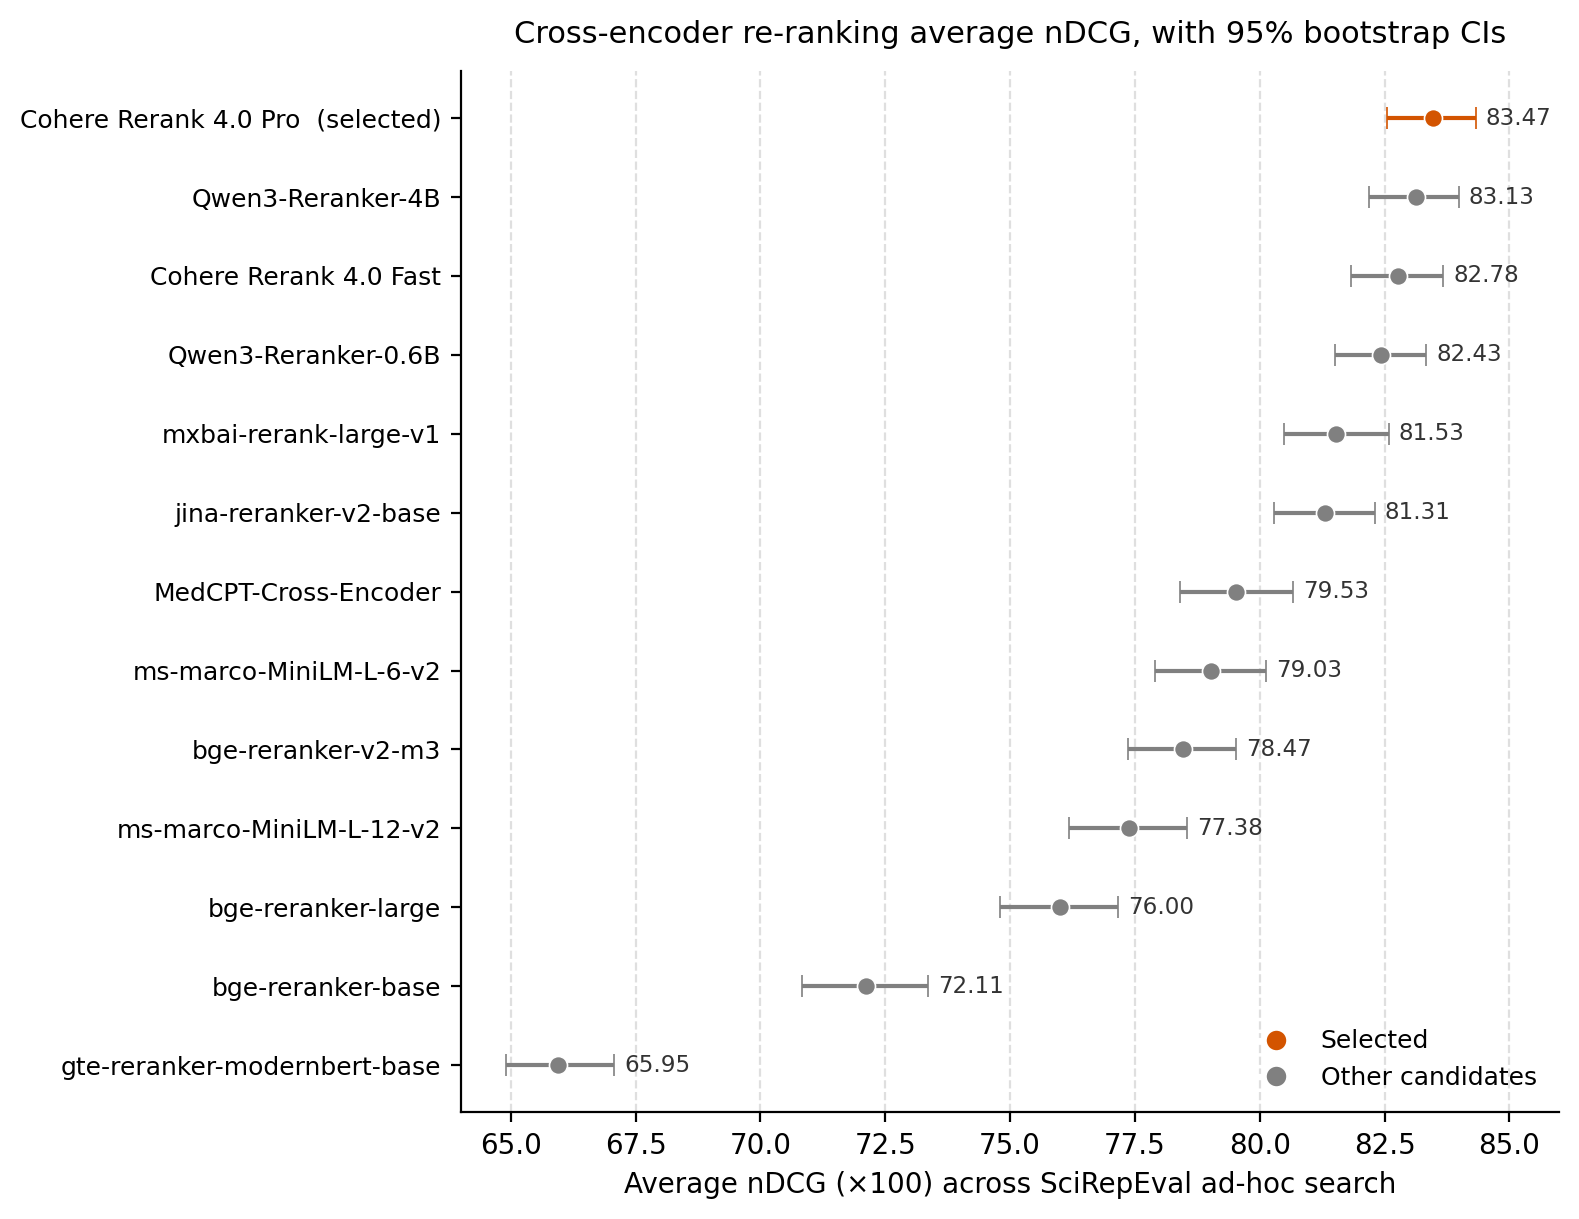
\includegraphics[width=\columnwidth]{images/data_and_results/crossencoder_average.png}
\caption{Cross-encoder re-ranking average nDCG across the three SciRepEval ad-hoc search tasks, with 95 percent bootstrap confidence intervals from 1000 resamples. The selected model is shown in orange.}
\label{fig:xenc-avg}
\end{figure}

\begin{figure}[t]
\centering
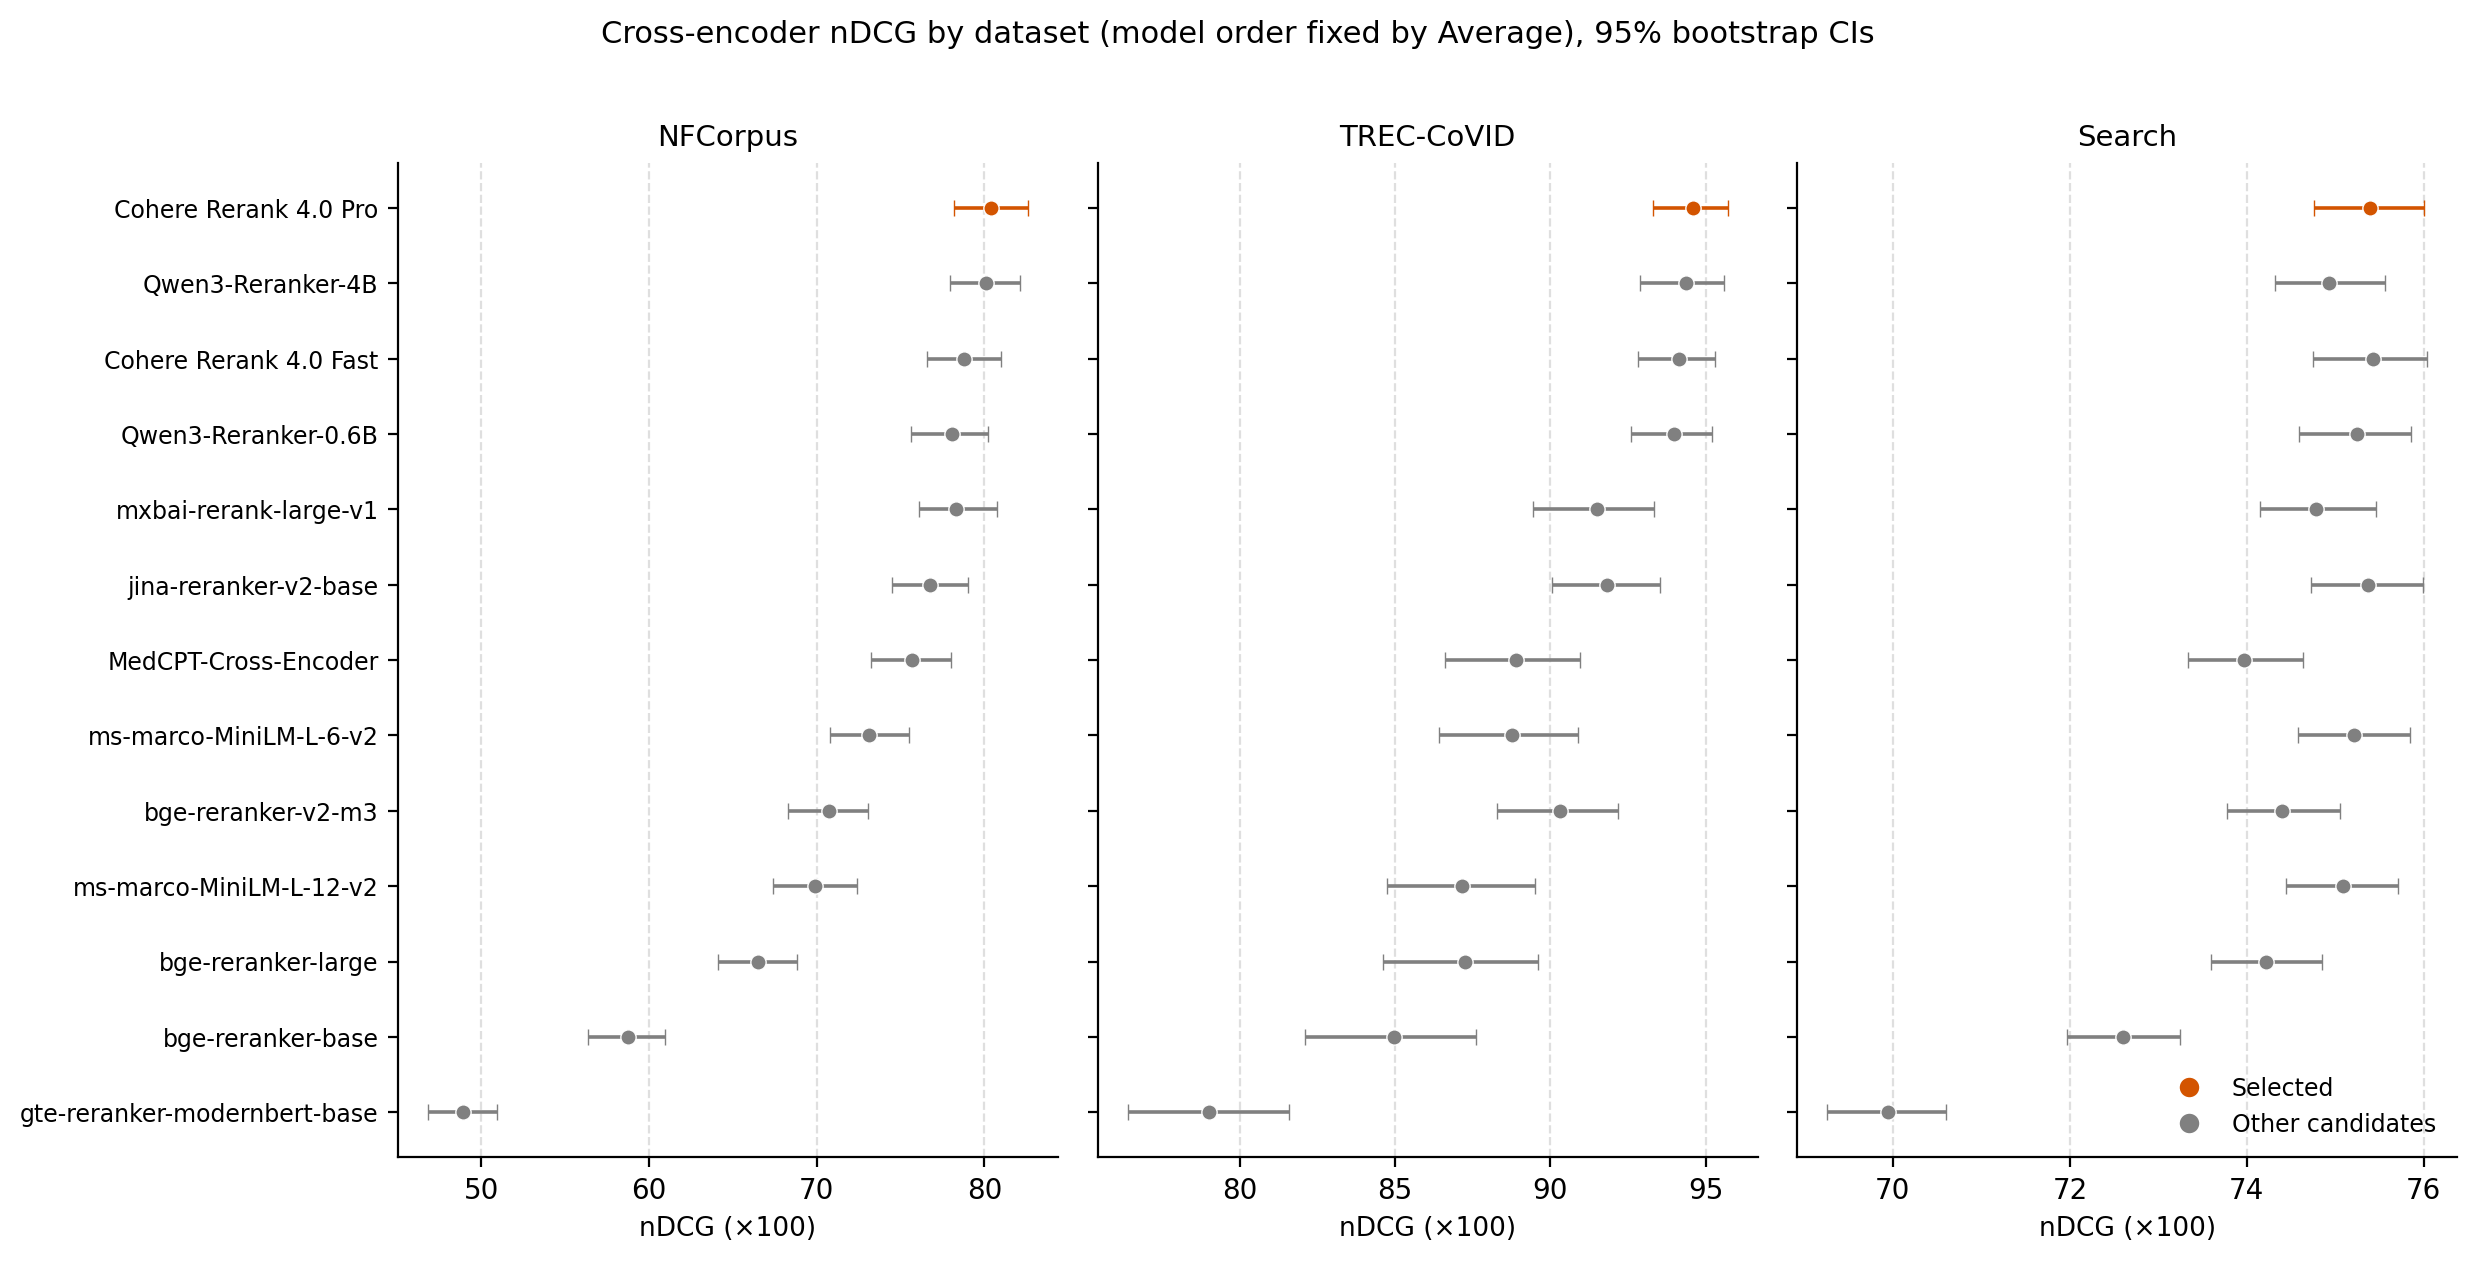
\includegraphics[width=\columnwidth]{images/data_and_results/crossencoder_by_dataset.png}
\caption{Cross-encoder nDCG on each SciRepEval ad-hoc search task, with models held in their Average order for comparison and 95 percent bootstrap confidence intervals. The selected model is shown in orange.}
\label{fig:xenc-pertask}
\end{figure}

Cohere Rerank 4.0 Pro was selected as the cross-encoder. The candidate rerankers were evaluated on the same three SciRepEval ad-hoc search tasks as the bi-encoder and under the same nDCG metric, scoring each model by the ranking it produces when it re-ranks the retrieved candidate pool. All scores are nDCG $\times$100 with 95 percent bootstrap intervals from 1000 resamples. The intervals are tight on Search, which has 2585 queries, and wide on TREC-CoVID, which has 50.

Table~\ref{tab:xenc-results} reports the full per-task and average scores, and Figure~\ref{fig:xenc-avg} plots each model's average with its interval. The selected model holds the highest average at 83.47. Its interval overlaps those of the next three models, Qwen3-Reranker-4B at 83.13, Cohere Rerank 4.0 Fast at 82.78, and Qwen3-Reranker-0.6B at 82.43, so these four form a statistical tie at the top. Within that group the strongest self-hostable model, Qwen3-Reranker-4B, is tied with the selected model. Below the leading four the field descends steadily through a long tail to gte-reranker-modernbert-base at 65.95, a spread of more than seventeen points from top to bottom.

The per-task view in Figure~\ref{fig:xenc-pertask} shows that almost all of this separation comes from NFCorpus, where the models spread across more than thirty points, from 80.42 at the top down to 48.88. Search behaves in the opposite way. Every reranker scores close to 75, since the small candidate pool the stage re-ranks leaves little room to reorder, so the task barely separates the models. TREC-CoVID falls between the two, with a high but noisy spread that reflects its fifty queries.

\begin{table*}[t]
\caption{Deployment characteristics of the candidate cross-encoders.}
\label{tab:xenc-deploy}
\centering
\footnotesize
\begin{tabular}{@{}p{4.5cm}llp{4.0cm}@{}}
\toprule
Model & Params (approx.) & Precision & Self-hostable \\
\midrule
Cohere Rerank 4.0 Pro & undisclosed & n/a & no (paid API) \\
Qwen3-Reranker-4B & $\sim$4 B & int8 & yes (Apache-2.0) \\
Cohere Rerank 4.0 Fast & undisclosed & n/a & no (paid API) \\
Qwen3-Reranker-0.6B & $\sim$0.6 B & fp16 & yes (Apache-2.0) \\
mxbai-rerank-large-v1 & $\sim$435 M & fp16 & yes \\
jina-reranker-v2-base & $\sim$278 M & fp16 & weights CC-BY-NC (non-commercial) \\
MedCPT-Cross-Encoder & $\sim$109 M & fp16 & yes \\
ms-marco-MiniLM-L-6-v2 & $\sim$22 M & fp16 & yes \\
bge-reranker-v2-m3 & $\sim$568 M & fp16 & yes \\
ms-marco-MiniLM-L-12-v2 & $\sim$33 M & fp16 & yes \\
bge-reranker-large & $\sim$560 M & fp16 & yes \\
bge-reranker-base & $\sim$278 M & fp16 & yes \\
gte-reranker-modernbert-base & $\sim$150 M & fp16 & yes \\
\bottomrule
\end{tabular}

\vspace{3pt}
\begin{minipage}{\linewidth}
\footnotesize\itshape
Unlike the bi-encoder, a reranker stores no vectors, so its cost is latency, which scales with parameter count, rather than memory, which is why the stage runs over only around 100 candidates. The Qwen3 rerankers are released under Apache-2.0, while the jina-reranker-v2 weights are CC-BY-NC-4.0 and so are non-commercial and not deployable in a commercial product. The remaining licences should be confirmed against the deployment terms before selection.
\end{minipage}
\end{table*}

Table~\ref{tab:xenc-deploy} records the deployment characteristics, namely approximate parameter count, precision, and whether the model is self-hostable along with its licence. Unlike the bi-encoder, a reranker stores no vectors, so its cost is latency rather than memory and scales with parameter count, which is the reason the stage runs over only around 100 candidates. The self-hostable options carry mixed licences, with the Qwen3 rerankers released under Apache-2.0 and the jina reranker under a non-commercial CC-BY-NC licence, while the selected model is served through a paid API.

% ----------------------------------------------------------------------------
\subsection{Embedding Quantisation}
% Placeholder. Results not yet available.
\textit{[Placeholder. Results comparing int8 against full-precision nDCG, and the resulting accuracy cost, to be added.]}

% ----------------------------------------------------------------------------
\subsection{System-Level Evaluation}
% Placeholder. Results not yet available.
\textit{[Placeholder. End-to-end results over a realistic query set with light relevance judgments to be added.]}